\documentclass[a4paper,12pt]{article}
\usepackage{titlesec}
\setcounter{secnumdepth}{4}
\setcounter{tocdepth}{4}
\usepackage[normalem]{ulem}
\useunder{\uline}{\ul}{}
%\usepackage[dutch]{babel}
\usepackage{fullpage}
\renewcommand{\baselinestretch}{1.5}
\usepackage[a4paper,margin=2.5cm]{geometry}
\usepackage{graphicx}
\usepackage{subfig}
%\graphicspath{{Images/}}
\usepackage{wrapfig}
\usepackage{floatrow}
\usepackage{rotating}
\usepackage{commath}
\usepackage{amsmath,amssymb}
\usepackage{amsfonts}
\usepackage{bm}
\usepackage{tablefootnote}
\usepackage{lipsum}
\usepackage{graphicx}
\usepackage{afterpage}
\usepackage{lscape}
\usepackage{apacite}
\usepackage{footnote}
\usepackage{float}
\floatstyle{plaintop}
\restylefloat{table}
\usepackage{caption}
%\captionsetup[table]{position=top}
\usepackage[toc,page]{appendix}
\usepackage{subcaption}
%\usepackage{subfigure}
\usepackage[bottom]{footmisc}
\usepackage{float}
\restylefloat{table}
%\floatsetup[table]{capposition=top}
\usepackage[skip=2pt,font=small]{caption}
\usepackage{listings}
\usepackage{pdflscape, afterpage}
\usepackage{multirow}
\usepackage[T1]{fontenc}
\usepackage[utf8]{inputenc}
\usepackage{tabularx,ragged2e,booktabs,caption}
\usepackage{enumerate}
\usepackage{float}
\usepackage{pdflscape}
\usepackage{afterpage}
\usepackage{amsthm}
\theoremstyle{plain}
\newtheorem{thm}{Theorem}
\newtheorem{mydef}{Definition}
\usepackage{color} %red, green, blue, yellow, cyan, magenta, black, white
\definecolor{mygreen}{RGB}{28,172,0} % color values Red, Green, Blue
\definecolor{mylilas}{RGB}{170,55,241}
\makeatletter
\newcommand{\distas}[1]{\mathbin{\overset{#1}{\kern\z@\sim}}}%
\newsavebox{\mybox}\newsavebox{\mysim}
\newcommand{\distras}[1]{%
  \savebox{\mybox}{\hbox{\kern3pt$\scriptstyle#1$\kern3pt}}%
  \savebox{\mysim}{\hbox{$\sim$}}%
  \mathbin{\overset{#1}{\kern\z@\resizebox{\wd\mybox}{\ht\mysim}{$\sim$}}}%
}
\titlespacing*{\paragraph}
{0pt}{3.25ex plus 1ex minus .2ex}{1.5ex plus .2ex}
%Includes "References" in the table of contents
\usepackage[nottoc]{tocbibind}
\usepackage{tocloft}
\usepackage{comment}
\usepackage[demo]{graphicx}
%\renewcommand\cftsecfont{\fontsize{10}}
%\renewcommand\cftsecafterpnum{\par\addvspace{6pt}}
\newcommand\blfootnote[1]{%
  \begingroup
  \renewcommand\thefootnote{}\footnote{#1}%
  \addtocounter{footnote}{-1}%
  \endgroup
}
\newenvironment{changemargin}[2]{%
  \begin{list}{}{%
    \setlength{\topsep}{0pt}%
    \setlength{\leftmargin}{#1}%
    \setlength{\rightmargin}{#2}%
    \setlength{\listparindent}{\parindent}%
    \setlength{\itemindent}{\parindent}%
    \setlength{\parsep}{\parskip}%
  }%
  \item[]}{\end{list}}

\makeatother
\begin{document}

\begin{center}
\pagenumbering{gobble}
\textsc{\LARGE Erasmus University Rotterdam}\\[0.9cm]
\textsc{\Large Econometrics \& Management Science}\\[0.9cm]
\textsc{\Large Thesis Quantitative Finance}\\[1cm]


% Title
\hrule
\vspace{0.5cm}
{ \Large \bfseries Comparing the Block Maxima and Peak over Threshold method for quantifying risk under serial dependence \\[0.4cm] }
\hrule
\vspace{1.5cm}

% Author and supervisor
\noindent
\begin{minipage}[t]{0.4\textwidth}
\begin{flushleft} \large
\emph{\textbf{Author:}}\\
M. \textsc{Nuis}\\
\smallskip
\emph{\textbf{Student Number:}}\\
\textsc{361830}\\
\end{flushleft}
\end{minipage}%
\begin{minipage}[t]{0.4\textwidth}
\begin{flushright} \large 
\emph{\textbf{Supervisor:}}\\
C. \textsc{Zhou}\\
\smallskip
\emph{\textbf{Second Assessor:}} \\
\\
\end{flushright}
\end{minipage}

\vspace{0.5cm}
{\large Date: \large \today\par}\\
\vspace{1cm}
\emph{\textbf{Abstract}}\\
\textit{To be added}\\ 
\vspace{0.5cm}
\hline
\vspace{0.5cm}
\textbf{Keywords:} 
\end{center}
\vspace{1cm}

\begin{figure}[h]

\includegraphics[width=8cm,height=50]{Figures/Logo_Erasmus_Universiteit_Rotterdam.png}
\end{figure}

\newpage
\pagenumbering{arabic}
\tableofcontents
\newpage

\section{Introduction}
A major aspect of quantitative risk management focuses on measuring risk. Over the years, this resulted in the development of a range of risk measures. The focus of this paper is primarily on the Value-at-Risk (VaR). The VaR measure is widely accepted within the banking industry as the preferred method for quantifying market risk. It plays an important role in the Basel Accords because the capital requirements of the banks are dependent on market risk. The accuracy of the VaR estimation is of great importance; an overestimation of the risk can lead to unnecessarily large capital allocations which could have been used elsewhere, and an underestimation can lead to extreme losses or even bankruptcy. However, during the financial crisis of 2008, it became apparent that the popular risk measure was not without flaws. As with many risk measures, the calculation of the VaR is based on assumptions which are often invalid with financial data. Another point of criticism is that the VaR is not able to implement other risk factors that influence the market risk such as liquidity, cash flow, counter-party and political risk. Hence, improving the estimation of the VaR is not only relevant from an academic standpoint, but also valuable to the financial industry. \newline

This paper will calculate the VaR for a diversified investment portfolio in European stocks and bonds. However, this portfolio contains serial dependence, which is generally the case for financial returns, and violates one of the assumptions used in calculating the VaR: that the observed data is independent and identically distributed (IID). The existing methods for calculating the VaR are analysed and compared after allowing for serial dependence. The comparison of the traditional VaR and the VaR after correcting for serial dependency is particularly interesting in times of extreme values, such as the 2008 financial crisis. \newline

Extreme Value Theory (EVT) has become increasingly popular in financial risk management because it only looks at the distribution of the tail rather than the whole distribution. Within EVT, the two dominant methods to estimate tail probabilities are the Block Maxima (BM) and the Peak Over Threshold (POT) approach. Both methods attempt to derive the limiting distribution of extreme values, but they differ in how the extreme values are chosen. The BM method divides the sample set into blocks of equal size and only considers the maximum values of these blocks, whereas the POT method only uses the extreme values that exceed a certain threshold. Both the BM and POT methods provide ways to infer high quantiles of the original data sample using the estimated distribution of the tails. However, one of the assumptions involved in estimating VaR using the classical POT or BM method is that the data sample is IID or exhibits weak dependence.\\

Various studies have analysed the application of the POT or BM method on serially dependent observations to estimate the tail distributions and calculate the VaR. It became apparent that both methods are able to deal with the serial dependency albeit with both advantages and disadvantages. \citeA{drees2003extreme} has demonstrated that the POT can still be used in the same approach to estimate the VaR when dealing with a serially dependent data sample and is therefore straightforward to implement. However, the estimates usually bear a higher asymptotic variance. The estimation of the VaR with serially dependent data can also be achieved using the BM method. In contrast with the POT method, the asymptotic properties of the estimators actually remain valid as the block maxima itself is arguably IID. However, \citeA{mcneil1998calculating} has demonstrated that estimating the VaR using BM requires the additional step of estimating the extremal index first. The extremal index is a parameter that characterises the serial dependence as it indicates the clustering of extreme values; see \citeA{leadbetter1983extremes}, for example. \\

Theoretically, it seems that the advantages and disadvantages of both the POT and BM approach to estimate the VaR under serially correlated data are roughly in balance. This conjecture needs to be proven, hence the following research question:\\

\noindent \textbf{`Which method is empirically most appropriate for estimating high quantiles under serial dependence?'}\\

This research paper compares both the BM and POT methods and tries to determine which method is most appropriate for estimating high quantiles under serial dependence. The research is based on a simulation study and an empirical study. We start with the simulation in order to fully analyse the performance of both methods on different levels of serial dependence. The data is generated using a Monte Carlo simulation in which the level of serial dependence is controlled. The simulation stays close to the empirical application by generating two time-series resembling stock and bond returns respectively. We first simulate two ARMA processes to mimic the univariate return series of the stock and bond returns that each contains serial dependence. We use a GARCH model for the innovations of each time-series to allow for the volatility clustering that is often present in financial returns. On each given day, the pair of the innovations from the two time-series, are simulated from a Clayton copula model to allow for cross-sectional dependence. This allows us to incorporate conditional tail dependency, which is in line with the joint distribution of the returns of a stock and bond portfolio. The BM and POT methods are then applied to estimate the $99.99\%$ VaR of the portfolio which invests equally weighted in the two return series. To estimate the VaR at such a high probability level, it is necessary to estimate the risk measures using EVT because a non-parametric estimation is not possible. The estimated VaR for every simulation sample are then compared with the true VaR which is obtained via a pre-simulation. To evaluate the BM and POT methods for each risk measure estimate, the average RMSE is calculated over the simulated samples. \\


In the empirical study, we apply the same BM and POT methods as in the simulation study to an investment portfolio that closely resembles the typical portfolio of a large bank. To evaluate the VaR estimates, we use the binomial method, see \citeA{christoffersen1998evaluating}. The binomial method is based on the number of observations that exceed the estimated VaR. Under the null hypothesis, the number of observations exceeding the $99.99\%$ VaR follows a binomial distribution with the probability of success equals $0.01\%$. \\

For the empirical application, we consider an investment portfolio consisting of the STOXX Europe 600 index and the Barclays Euro Aggregate Treasury Total Return Index, to represent the stock and bond markets respectively. The data consists of daily observations starting from January 1, 2000 till December 31, 2017. This period is interesting as it contains two major financial crises: the burst of the dot-com bubble and the 2008 global financial crisis.\\

The remainder of this paper is structured as follows. Section 2 discusses the current literature. The methodology is outlined in section 3, where the POT and BM methods are discussed, and the simulation setup is described. Section 4 closely examines the empirical data. The performance of both methods are analyzed and discussed in Section 5. Section 6 concludes the research.

\newpage
\section{Literature}
EVT is a field of research within statistics that primarily focuses on the stochastic behaviour of extreme values in a process. The history of EVT dates all the way back to Bernoulli in 1709 as demonstrated by \citeA{kotz2000extreme}. Over the years, EVT has evolved and currently relies mainly on two distinct methods to model the distribution of extreme values: the BM and the POT method. Between the two, the BM method has been around for longer. It was first mentioned in \citeA{fisher1928limiting}, who indicated that the limiting behavior of maxima can be described by a set of three extreme value distributions: the Gumbel, Fr\'echet, and the inverse Weibull distributions. \\

Denote $X_1, \dots, X_n$ as the IID observations with cumulative distribution function (CDF) $F$ and $M_n = \max\left(X_1,\dots\,X_n\right)$. Then, assume that 
\begin{equation}
\Pr\left(\frac{M_n-b_n}{a_n}\leq x\right)=F^n\left(a_nx+b_n\right)\to G\left(x\right),
\end{equation}

\noindent for some constants $a_n$ and $b_n$ as $n\to\infty$. Similar to the Central Limit Theorem, the normalised maxima converges to the distribution $G$. The Extremal Types Theorem (\citeA{fisher1928limiting}; \citeA{gnedenko1943distribution}) states that the limit distribution $G$ can only be one of the following types:

\begin{equation*}
    \begin{split}
        \text{Type I:} \quad & \quad G(x) = \exp{\left(-\exp{\left(-x\right)}\right)}, \quad \text{for} \quad x\in\mathbb{R}, \\
        \text{Type II:} \quad & \quad G(x) = \begin{cases} 0 \quad\quad\quad\quad\quad \text{if} \quad x < 0,\\ \exp{\left(-x^{-a}\right)} \quad \text{if} \quad x\geq 0, \end{cases}\\
        \text{Type III:} \quad & \quad G(x) = \begin{cases} \exp{\left(-\left(-x\right)^a\right)} \quad \text{if} \quad x < 0,\\ 1 \quad\quad\quad\quad\quad\quad \text{if} \quad x\geq 0, \end{cases}
    \end{split}
\end{equation*}
where for type II and III it holds that $a>0$. These three types are referred to as the Gumbel, Fr\'echet and the inverse Weibull distributions respectively. \citeA{gnedenko1943distribution} shows that these three CDFs can be generalised into one distribution function, which is called the Generalized Extreme Value (GEV) distribution, see equation \eqref{eq:GEV} below. Hence, the maxima from a sample of observations approximately follow the GEV distribution, and the type of distribution is dependent on the shape parameter $\xi$. \\

The most notable methods of estimating the parameters of the GEV distribution are the maximum likelihood estimation by \citeA{prescott1980maximum} and the probability weighted moments by \citeA{hosking1985estimation}. After fitting the GEV distribution to the block maxima using maximum likelihood, \citeA{mcneil1998calculating} demonstrates that the relation between the high quantile of the block maxima, sometimes referred as the return level, and a high quantile of the observations only depends on the probability level and the block size of the block maxima. In the same paper, the estimation of high quantiles on serially dependent data is analysed, with the finding that the BM method cannot be applied directly to the serially dependent case. This is due to the extremal index parameter, which indicates the degree of clustering of extreme values; see \citeA{leadbetter1983extremes} for a more detailed theoretical interpretation. The relation between the high quantiles of the block maxima and the high quantiles of the observations is now also dependent on this extremal index. Hence, the extremal index needs to be estimated first in order to obtain a high quantile of serially dependent data. The estimation of the extremal index under stationary and weak dependence has been performed by \citeA{hsing1993extremal} and \citeA{smith1994estimating}. More recently, \citeA{berghaus2018weak} provided an improved version of the maximum likelihood estimator by \citeA{northrop2015efficient}, by incorporating sliding block maxima.\\

The POT method has recently gained significant popularity over the BM method. The POT differs from the BM method in the way the extreme values (from which we try to obtain the limiting distribution) are chosen. The POT only considers the extreme values that exceed a certain threshold. One of the advantages that has repeatedly been mentioned is the fact that the POT method uses all the extreme values. As the BM method only considers the maximum in a range of values, it may waste extreme values. This feature is even more strongly present in the case of non-IID data, as extreme values are usually more clustered together. Assume $X-u$ to be the excess losses. Then, using the general rules of conditional probability, the distribution of the excess losses can be described as $F_u(x) &= P(X-u\leq x| X > u) = \frac{F(x+u) - F(u)}{1 - F(u)}$. It then follows that the excess distribution function $F_u$ can be approximated by the Generalized Pareto Distribution (GPD); see equation \eqref{eq:POT}. The theorem behind this is derived from \citeA{balkema1974residual} and \citeA{pickands1975statistical}. Hence, the excess losses above a high threshold follow approximately the GPD distribution. The shape parameter in the GPD distribution is identical to the shape parameter of the GEV distribution.\\

As with the BM method, the most important methods for estimating the parameters of the GPD distribution are the maximum likelihood and the probability weighted moments, which are both discussed in \citeA{hosking1987parameter}. \citeA{smith1987estimating} has extensively investigated the tail estimation based on IID data and has derived the theoretical properties of the maximum likelihood estimator based on POT. When the limit of the maxima is of type II, another method to estimate the shape parameters is the Hill estimator by citeA{hill1975simple}. Hence, high quantiles of the data can be estimated through the estimated parameters of the GPD and the inverse CDF or by extrapolating a less extreme quantile to a high quantile using the reciprocal of the shape parameter. Both methods are described by \citeA{mcneil2005quantitative}. In the case of non-IID data, \citeA{drees2003extreme} has demonstrated that the derived methods can still be used. However, the asymptotic variance is different from, usually higher than, the IID case. \citeA{drees2003extreme} also provides a theoretical estimator for the asymptotic variance.

\newpage
\section{Methodology}
\subsection{Value-at-Risk}
Before discussing the BM and POT methods in further detail, a formal definition of the VaR is needed. The VaR is a quantitative risk measure that is usually applied on the loss distribution. In probabilistic terms, the VaR can be interpreted as the quantile of this loss distribution. A great definition is given by \citeA{mcneil2005quantitative} as follows
\begin{mydef}{\textbf{(Value-at-Risk).}}
    Given some confidence level $p \in \left(0,1\right)$. The VaR of the losses at the confidence interval $p$ is given by the smalles number $l$ such that the probability that the loss $L$ exceeds $l$ is no larger than $\left(1-p\right)$. Formally, 
    \begin{equation}
        VaR_p=\inf\{l\in\mathbb{R}: P\left(L>l\right)\leq 1-p\}=\inf\{l\in\mathbb{R}: F_L\left(l\right)\geq p\}.
    \end{equation}
\end{mydef}
\noindent It is common to use high values for $p$ such as $p=0.95$ or $p=0.99$. The focus of this paper lies in extreme values and inferring high quantiles using EVT. Therefore, the confidence level of interest throughout this paper is chosen to be $p=0.9999$. The major drawback of the VaR as a risk measure is that the VaR does not give any information about the extreme losses that occur with probability less then $1-p$.

\subsection{Extreme Value Theory}

\subsection{Block Maxima}
This section first discusses the BM method for the IID case, before the theory is extended to serially dependent data. The BM method has been fundamental and is considered to be one of the oldest models within EVT. It is essential to discuss the probability theory behind the convergence of maxima before deriving the estimators in the BM method. Assume a set of IID random variables denoted as $X_1, X_2, \dots$ with distribution function $F$ and define the maximum as $M_n=\max\left(X_1, \dots, X_n\right)$. The EVT considers the limiting distribution of $M_n$. Assume that with normalising constants $a_n$ and $b_n$, $M_n$ converge in distribution as $n\to \infty$, i.e.

\begin{equation}
    \lim_{n\to\infty} P\left(\frac{M_n-b_n}{a_n}\leq x\right)=\lim_{n\to\infty}F^n\left(a_nx+b_n\right)=H\left(x\right),
    \label{eq:maximumdomain}
\end{equation}
where $H\left(x\right)$ is a non-degenerate distribution function. Here, a non-degenerate distribution function is a limiting distribution that is not concentrated on a single point. If the condition \eqref{eq:maximumdomain} holds, then $F$ is said to be in the maximum domain of attraction of $H$, which can be written as $F\in MDA\left(X\right)$. In a similar manner as the Central Limit Theorem for averages, the Extremal Types Theorem for maxima of \citeA{fisher1928limiting} and \citeA{gnedenko1943distribution} states that in case the distribution of a normalized maximum converges, the limiting distribution has to be one of a particular class of distributions.

\begin{thm}{\textbf{(Fisher-Tippett, Gnedenko).}}
    If $F\in MDA\left(X\right)$ for some non-degenerate distribution function $H$, then $H$ must be a Generalized Extreme Value (GEV) distribution distribution defined as
\end{thm}

\begin{equation}
    H_{\xi}(x) = \begin{cases}
               \exp{\left(-\left(1+\xi x\right)^{-\frac{1}{\xi}}\right)} \quad \textrm{for} \quad \xi\neq0,\\
              \exp{\left(-\exp{\left(-x\right)}\right)} \quad\quad \textrm{for} \quad \xi=0
            \end{cases}
\label{eq:GEV}
\end{equation}
where $1+\xi x > 0$. A three-parameter family is obtained by defining $H_{\xi, \mu, \sigma}\left(x\right):=H_{\xi}\left(\frac{x-\mu}{\sigma}\right)$ where $\sigma>0$ and $\mu$, $\xi \in \mathbb{R}$. The parameters $\mu$, $\sigma$ and $\xi$ are referred to as the location, scale, and shape parameter respectively. Two examples of obtaining the GEV are given in the Appendix \ref{appendixA:maximumdomain}, with $F$ following the exponential distribution and the Pareto distribution. Depending on the value of $\xi$, the distribution $H_\xi$ defines a type of distribution. There are three possible states of $\xi$ that each correspond to one of the three types of extreme value distributions. Figure \ref{fig:gev} displays the three different extreme value distribution families for which it holds that

\begin{itemize}
    \item $\xi=0$: Gumbel or type I extreme value distribution
    \item $\xi>0$: Fr\'echet or type II extreme value distribution
    \item $\xi<0$: Weibull or type III extreme value distribution.
\end{itemize}

\begin{figure}[H]
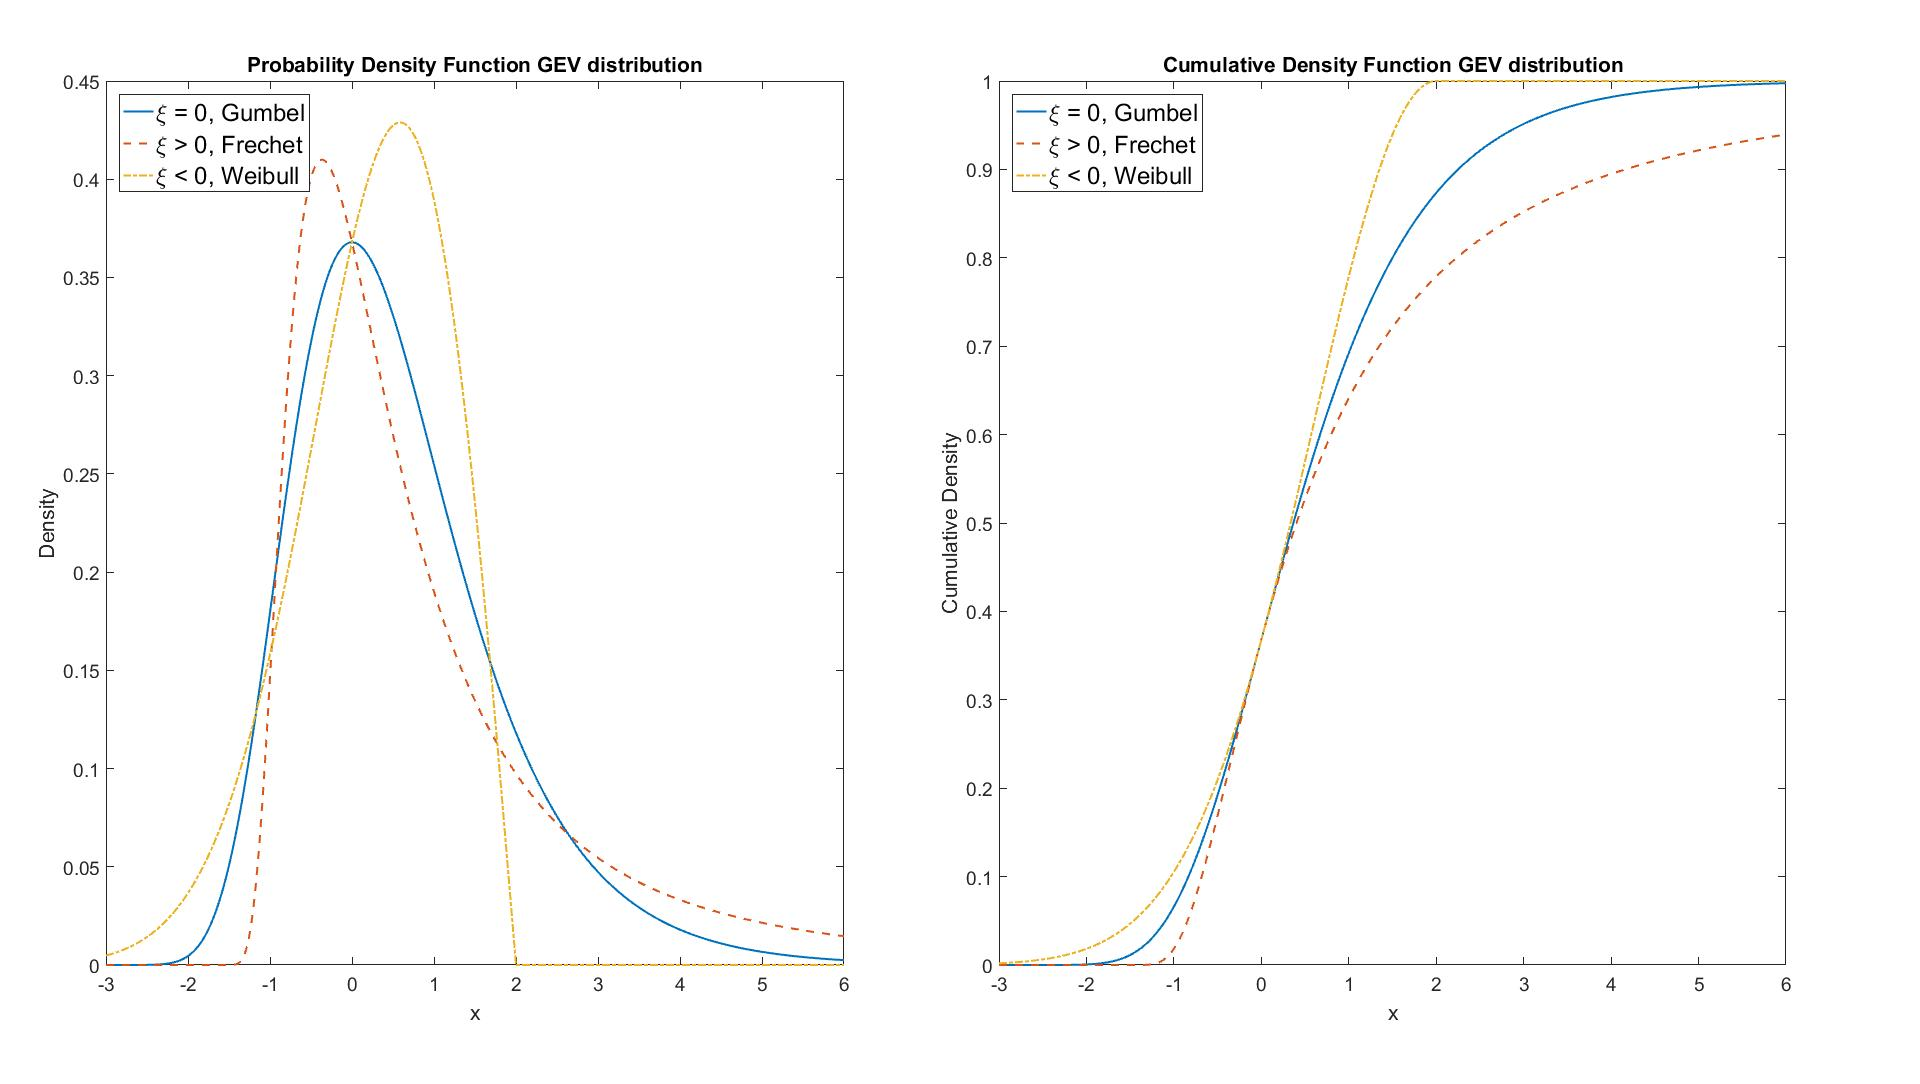
\includegraphics[height=7.8cm, width=\linewidth]{Figures/gev.jpg} 
\caption{The probability density function (PDF) and CDF for three different values of $\xi$ and $\mu=0$ and $\sigma=1$. The solid line corresponds to $\xi=0$ (Gumbel); the dashed line is $\xi=0.5$ (Fr\'echet) and the dotted-dashed line is $\xi=-0.5$ (Weibull).}
\label{fig:gev}
\end{figure}

The Weibull distribution is considered a short-tailed distribution with a finite right endpoint denoted by $x_F=\sup\{x\in\mathbb{R}: F(x) < 1\}$. This class of distributions are usually not that interesting when quantifying financial risk as the distribution of losses is often considered heavy-tailed. Both the Gumbel and Fr\'echet distributions are heavy-tailed distributions with infinite right endpoints. Within the Gumbel class there are many distributions for example: the normal, lognormal, gamma and chi-squared distribution. The Fr\'echet distribution has a lower decay of the right tail than the Gumbel distribution and consists of heavy-tailed distributions, for example the Pareto distribution. These distributions are also known as the power-tailed distributions and are often the preferred choice in modeling losses.\\

The aim of this paper is to infer high quantiles on financial losses containing serial dependence. Since financial losses are known to be heavy-tailed, see \citeA{mandelbrot1963new}, we restrict the research to the class of Fr\'echet distributions or equivalently $\xi>0$. To estimate the parameters, the BM method divides the data with total number of observations $N$ into $k$ equally-sized blocks, each containing $n$ observations. Taking the maximum of each block generates a new sample that contains extreme values. Define the sample of block maxima formally as $\bm{M_n}=\{M_{n,1}, \dots, M_{n,k}\}$ where $M_{n,i}$ denotes the $i$th block maxima. Then, the block maxima follow approximately a GEV distribution $H_{\xi,\mu\sigma}$. The choice of the block size, $n$, and the corresponding number of blocks, $k$, has a significant impact in estimating the parameters of the GEV distribution. A large block size will lead to a more accurate approximation of the block maxima distribution by a GEV following the limit relation. Consequently, the parameter estimates have a lower bias. On the other hand, adopting a large $k$ will increase the number of block maxima. Therefore, the estimated parameters have a low variance. A visual interpretation of the BM method is indicated in Figure \ref{fig:blockmaxima}.

\begin{figure}[H]
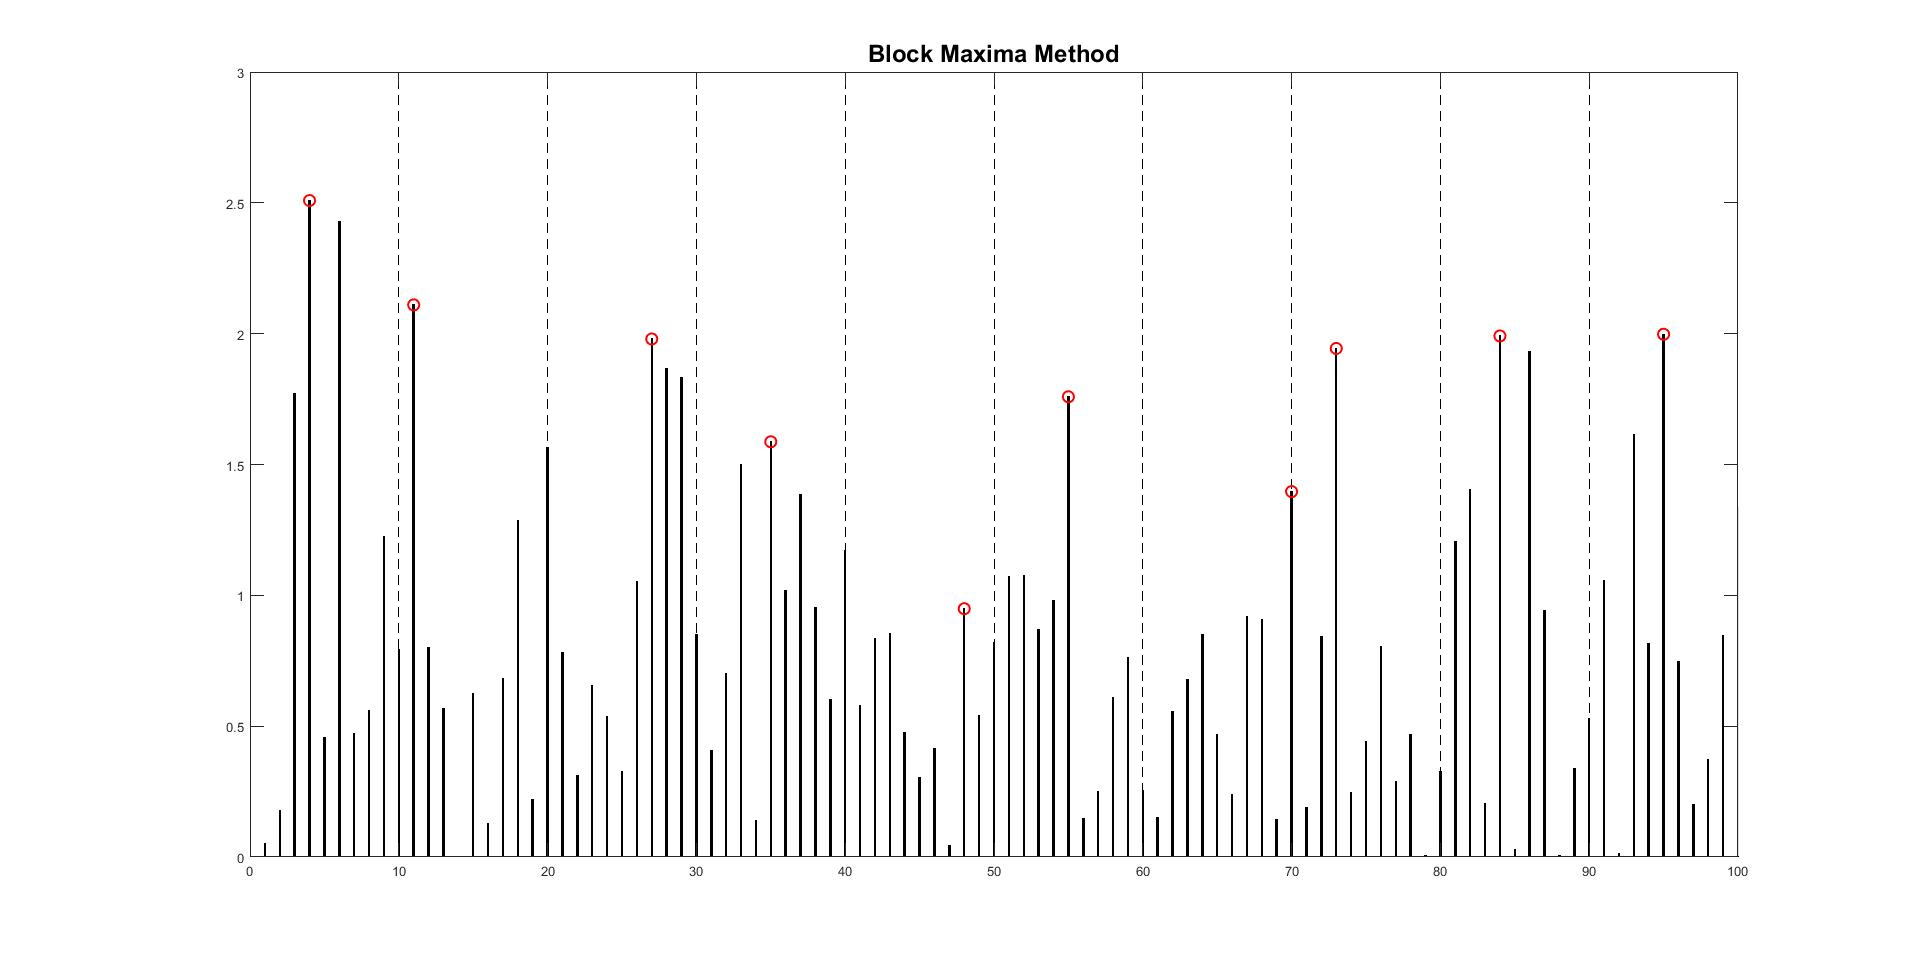
\includegraphics[height=7.8cm, width=\linewidth]{Figures/blockmaxima_example2.jpg} 
\caption{Visual interpretation of the BM method. The total number of observations $N$ equals 100 and is divided in $k=10$ blocks of $n=10$ observations where only the maximum values per block size are considered.}
\label{fig:blockmaxima}
\end{figure}

To estimate the parameters of the GEV distribution, either of the following two estimators is usually used: the maximum likelihood (ML) estimators, see \citeA{prescott1980maximum} and \citeA{bucher2018maximum}, and the probability weighted moment (PWM) estimators, see \citeA{hosking1987parameter} and \citeA{ferreira2015block}. In this study, we use maximum likelihood both in the BM as the POT approach in order to make a fair comparison. This paper adopts the estimators derived in \citeA{bucher2018maximum}, where the Fr\'echet distribution is used and the location parameter is set to zero. Here, we first explain the application of the maximum likelihood estimators for the Fr\'echet distribution in detail. \\

The CDF of the Fr\'echet distribution can be obtained via the GEV distribution \eqref{eq:GEV} by using $\xi>0$ and $y=1+\xi x$ and is thus defined as 
\begin{equation}
    F_{\xi}(y) = \begin{cases}
               \exp{\left(-y^{-\frac{1}{\xi}}\right)} \quad \textrm{for} \quad y > 0,\\
              0 \quad\quad\quad\quad\quad \textrm{for} \quad y\leq0
            \end{cases}
\label{eq:frechet}
\end{equation}
We focus on the two-parameter Fr\'echet distribution, similar to \citeA{bucher2018maximum}, which is obtained by $F_{\xi, \sigma}\left(y\right):=F_{\xi}\left(\frac{y}{\sigma}\right)$ and with CDF
\begin{equation}
    F_{\xi, \sigma}\left(y\right) = \exp{\left(-\left(\frac{y}{\sigma}\right)^{-\frac{1}{\xi}}\right)} \quad \textrm{for} \quad y > 0.
    \label{eq:frechetcdf}
\end{equation}
The PDF can be obtained by taking the first order derivative of the CDF.
\begin{equation}
    \begin{split}
    f_{\xi, \sigma}\left(y\right) &= \frac{\delta F_{\xi, \sigma}(y)}{\delta y} \\
    &= \frac{1}{\xi\sigma}\left(\frac{y}{\sigma}\right)^{-\frac{1}{\xi} -1}\exp{\left(-\left(\frac{y}{\sigma}\right)^{-\frac{1}{\xi}}\right)}.
    \end{split}
    \label{eq:gevpdf}
\end{equation}
Let $y=\left(y_1,\dots,y_k\right)\in \left(0, \infty\right)^k$ be a sample vector to which the Fr\'echet distribution is to be fitted. Then the log-likelihood can derived as
\begin{equation}
\begin{split}
    & l\left(\xi,\sigma;y_1, \dots, y_n\right) \\
    & = \sum_{i=1}^{k}\ln{\left(f_{\xi,\sigma}\left(y_i\right)\right)} \\
    & = -k\left(\ln{\left(\xi\right)}+\ln{\left(\sigma\right)}\right)-\sigma^{\frac{1}{\xi}}\sum_{i=1}^k y_i^{-\frac{1}{\xi}} - \left(\frac{1}{\xi}+1\right)\left(\sum_{i=1}^k \ln{\left(y_i\right)} - k\ln{\left(\sigma\right)}\right).
    \label{eq:frechetll}
\end{split}
\end{equation}
The maximum likelihood estimators $\hat{\xi}$, $\hat{\sigma}$ are obtained by maximizing \eqref{eq:frechetll} to the respective parameter. \citeA{bucher2018maximum}, derived the maximum likelihood estimators for the shape and scale parameter and established the consistency and asymptotic normality for the maximum likelihood estimators for both IID and strictly stationary time series. The maximum likelihood estimators for the scale parameter $\sigma$ and shape parameter $\xi$ are obtained as follows
\begin{equation}
    \hat{\sigma} = \left(\frac{1}{k}\sum^k_{i=1}y_i^{-\frac{1}{\hat{\xi}}}\right)^{-\hat{\xi}},
    \label{eq:bmmlsigma}
\end{equation}
\noindent where $\hat{\xi}$ is solution of $\Psi_k\left(\xi|y\right)=0$, with $\Psi_k\left(\xi|y\right)$ defined as
\begin{equation}
        \Psi_k\left(\xi|y\right) = \xi + \frac{\frac{1}{k}\sum^k_{i=1}y_i^{-\frac{1}{\xi}}\ln{\left(y_i\right)}}{\frac{1}{k}\sum^k_{i=1}y_i^{-\frac{1}{\xi}}} - \frac{1}{k}\sum^k_{i=1}\ln{\left(y_i\right)}.
        \label{eq:bmmlshape}
\end{equation}
If $\xi>0$, the block maxima $\bm{M_n}$ approximately follow the Fr\'echet distribution. The parameters can be estimated by replacing the sample vector $y$ by $\bm{M_n}$ in above derived estimators. After obtaining parameter estimates, we estimate the quantiles of the block maxima $\bm{M_n}$ by inverting the CDF and using the maximum likelihood parameters. \\

The relation between the VaR of the block maxima, which is sometimes referred to as the return level, and the VaR of the original observations is demonstrated by \citeA{mcneil1998calculating}. Because the VaR of the block maxima is a quantile on extreme values, it is therefore a high quantile of the original data. When the data are IID, the probability level corresponding to the VaR of the block maxima can then be calculated as

\begin{equation}
    \Pr\left(M_{n,i}<VaR_p\right)=\left(\Pr\left(X<VaR_p\right)\right)^n=p^n.
    \label{eq:relationrlvar}
\end{equation}
That is, the VaR is a quantile of the block maxima with probability level $p^n$. Therefore, using the inverse of equation \eqref{eq:frechetcdf} and parameter estimates \eqref{eq:bmmlsigma} and \eqref{eq:bmmlshape} we can estimate the VaR as
\begin{equation}
    \widehat{VaR}_p = \hat{\sigma}\left(-\ln{\left(p^n\right)}\right)^{-\hat{\xi}}
    \label{eq:bmestvariid}
\end{equation}

\\

When moving away from IID data and allowing for serial dependence, the convergence of the maxima follows a GEV distribution raised to the power $\theta$ as illustrated by \citeA{mcneil1998calculating}:

\begin{equation}
    \lim_{n\to\infty} P\left(\frac{\tilde{M}_n-b_n}{a_n}\leq x\right)=H^{\theta}\left(x\right),
\end{equation}

\noindent where we use $\tilde{M}_n$ to indicate that the data contains serial dependence and where $\theta$ in $\left(0, 1\right]$ is the so-called extremal index. Assuming that the maxima $\tilde{M}_n$ is obtained from a stationary series with the same distribution function $F$ as in the IID case ($M_n$); the distribution of $H_{\xi}^{\theta}\left(x\right)$ is of the same type as $H_{\xi}\left(x\right)$ with the exact same $\xi$ parameter. However, the location and scale parameter are different in this case. The extremal index is an important parameter that measures the degree of clustering of extremes in a stationary process.\\

\citeA{mcneil1998calculating} states that for large $n$ and $u=a_nx+b_n$ it now holds that $P\left(M_n\leq u\right)\approx P^{\theta}\left(\tilde{M}_n\leq u\right)=F^{n\theta}\left(u\right)$ so that for $u$ large the probability distribution of the maximum of $n$ observations from the time series with extremal index $\theta$ can be approximated by the distribution of the maximum of $n\theta<n$ observations from the associated IID time series. In a sense, $n\theta$ can be thought of as counting the number of roughly independent clusters of observations in $n$ observations. The extremal index $\theta$ is often interpreted as the reciprocal of the mean cluster size.
\\

Due to the serial dependence, the relation changes between the VaR of the block maxima and the VaR of the original observations and are now dependent on the extremal index. Demonstrated by \citeA{mcneil1998calculating}, the equations \eqref{eq:relationrlvar} and \eqref{eq:bmestvariid} now becomes
\begin{equation}
    \Pr\left(M_{n,i}<VaR_p\right)=\left(\Pr\left(X<VaR_p\right)\right)^{n\theta}=p^{n\theta},
    \label{eq:relationrlvar2}
\end{equation}
\noindent and
\begin{equation}
    \widehat{VaR}_p = \hat{\sigma}\left(-\ln{\left(p^{n\hat{\theta}}\right)}\right)^{-\hat{\xi}}.
    \label{eq:bmestvarserialdep}
\end{equation}
\\

When dealing with serial dependence, we need to estimate the extremal index first. \citeA{berghaus2018weak} has recently analyzed estimators for the extremal index based on disjoint and sliding block maxima. They derived the asymptotic normality and revealed that the sliding block estimator, outperforms other block estimators. Hence, we will adopt the sliding block estimators as proposed by \citeA{berghaus2018weak}:

\begin{equation}
    \hat{\theta}^{(1),sl}_n=\left(\frac{1}{k}\sum^{k}_{i=1}\hat{Z}^{sl}_{n,i}\right)^{-1}, \quad \hat{\theta}^{(2),sl}_n=\left(\frac{1}{k}\sum^{k}_{i=1}\hat{Y}^{sl}_{n,i}\right)^{-1},
    \label{eq:estextremalindex}
\end{equation}
where 
\begin{equation*}
    \hat{Z}^{sl}_{n,i}=n\left(1-\hat{W}^{sl}_{n,i}\right) \quad \text{and} \quad \hat{Y}^{sl}_{n,i}=-n\log\left(\hat{W}^{sl}_{n,i}\right)
\end{equation*}
with
\begin{equation*}
    \hat{W}^{sl}_{n,i}=\hat{F}_n\left(M^{sl}_{n,i}\right).
\end{equation*}
Here, $\hat{F}_n$ is the empirical CDF of the observations $X_1, \dots, X_N$. The sliding block maxima are obtained by dividing the sample of observations into $N-n+1$ blocks of length $n$, such that $M^{sl}_{n,i}=\max\left(X_{i},\dots,X_{i+n-1}\right)$ for $t=1,\dots,N-n+1$.
\\

To summarize, when dealing with IID data, the VaR can be estimated using equation \eqref{eq:bmestvariid}. Here, the relation between the quantiles of the block maxima and that of the original observations, and the estimated scale, and shape parameters are used. These parameters are often estimated using either maximum likelihood or probability weighted moment. In this paper we obtain the maximum likelihood parameters with equation \eqref{eq:bmmlsigma} and \eqref{eq:bmmlshape}. If the data is a strictly stationary time series, the scale parameter may change but the shape parameter is exactly the same. The relation between the quantiles of the block maxima and that of the original observations now depends on the extremal index. Under serial dependence, the VaR estimator now changes to equation \eqref{eq:bmestvarserialdep} using equation \eqref{eq:estextremalindex} to estimate the extremal index.

\subsection{Peak over Threshold}
A major disadvantage of the BM method is that it potentially neglects extreme values in the tails. This is because only the maximum of a group of data is used to estimate the GEV distribution. The existence of serial dependency within the data magnifies this shortcoming. This gave rise to the POT, another often-used method in EVT, that considers the extreme observations that exceed a certain threshold as illustrated in Figure \ref{fig:peakoverthreshold}. This section begins with discussing the theory of the POT method under the IID case. Afterwards, the IID assumption is relaxed and the differences are analysed. \\

\begin{figure}[H]
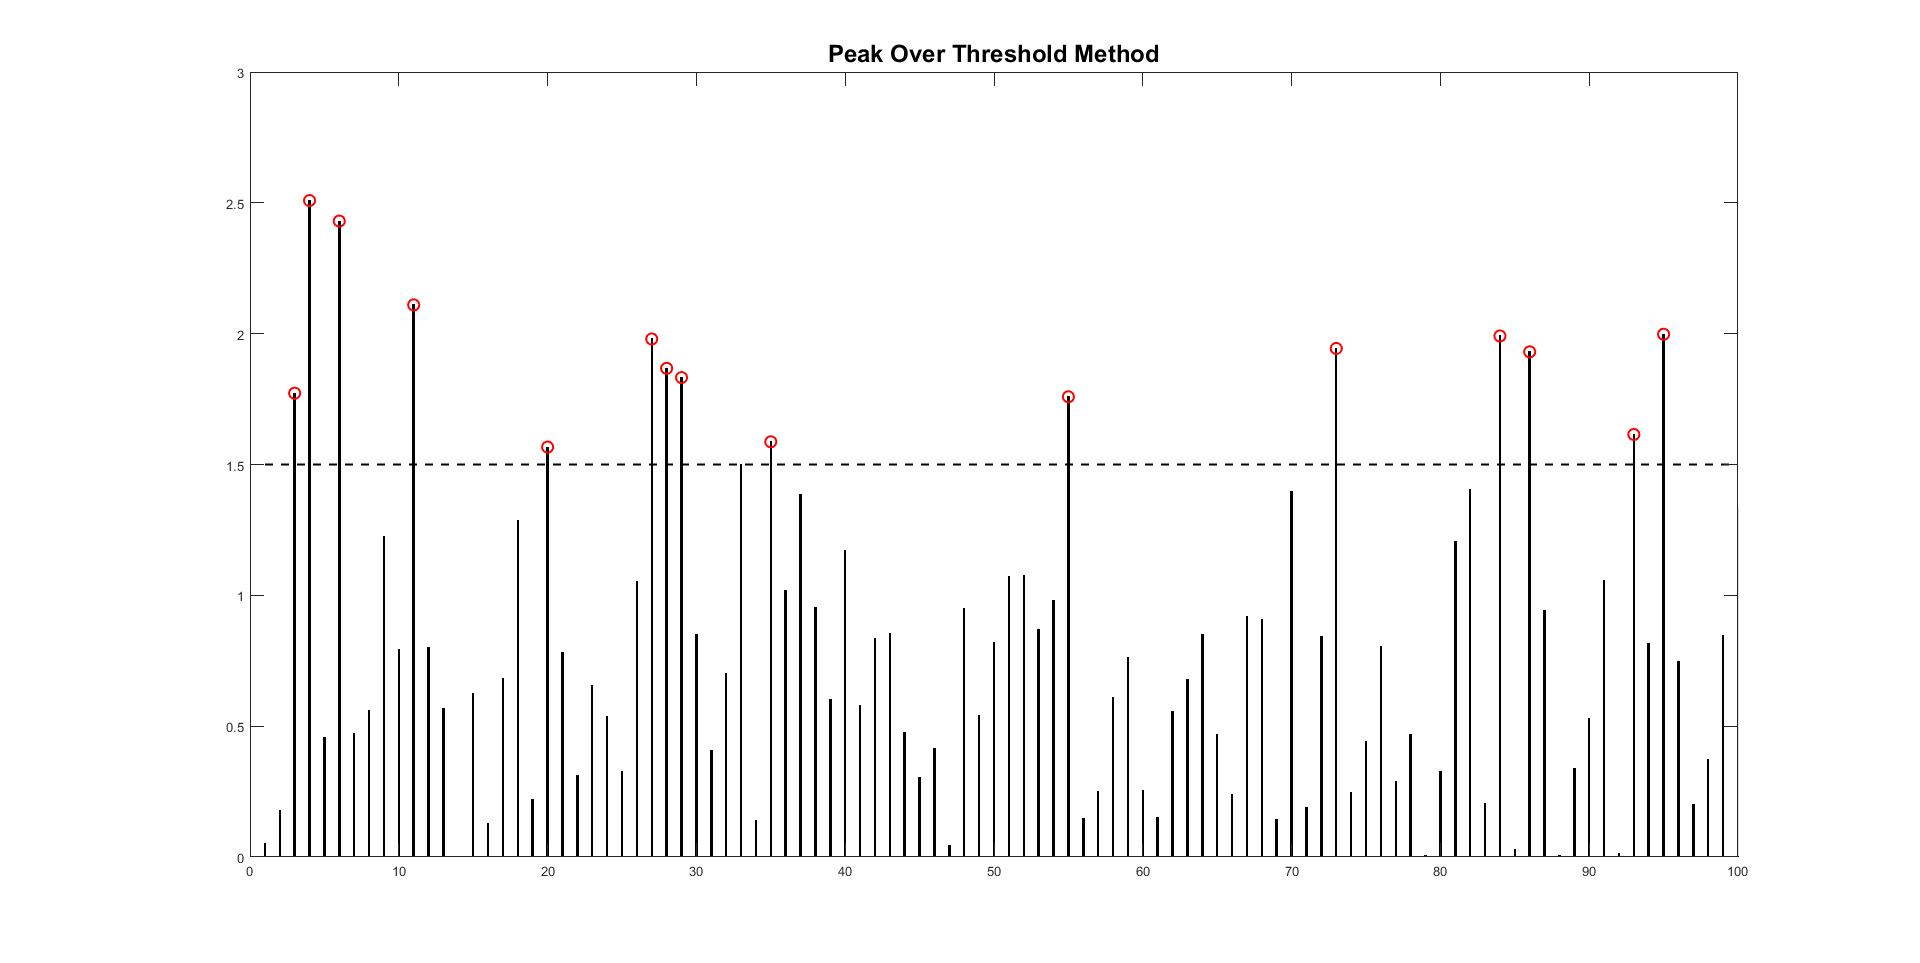
\includegraphics[height=7.8cm, width=\linewidth]{Figures/peakoverthreshold_example2.jpg} 
\vspace{-0.8cm}
\captionsetup[figure]{font=small,labelfont=small}
\caption{Visual interpretation of the POT method. Only the values exceeding the threshold of 1.5 are considered.}
\label{fig:peakoverthreshold}
\end{figure}

Let the losses $X$ be a random variable with possibly unknown distribution function $F$ such that $F(x) = P(X \leq x)$. We then define the CDF $F_u(x)$ for the excess losses $X-u$, given that the losses exceed the threshold $u$ as 

\begin{equation}
    \begin{split}
        F_u(x) &= P(X-u\leq x| X > u)\\
        & = \frac{F(x+u) - F(u)}{1 - F(u)},
    \end{split}
\end{equation}
for $0\leq x < x_F - u$, where $x_F\leq \infty$ is the right endpoint of $F$.\\

The theorem of Pickands-Balkema-de Haan, derived in \citeA{balkema1974residual} and \citeA{pickands1975statistical}, states that for a large class of underlying distributions $F$, the excess distribution function $F_u$ can be approximated by the GPD for an increasing threshold $u$. Hence, the observations exceeding the threshold follow a GPD with the following CDF:

\begin{equation}
    G_{\mu, \sigma, \xi}(x) = \begin{cases}
               1 - (1 + \xi\frac{x-\mu}{\sigma})^{-\frac{1}{\xi}} \quad \textrm{for} \quad \xi\neq0,\\
               1 - e^{-\frac{x-\mu}{\sigma}} \quad \textrm{for} \quad \xi=0,
            \end{cases}
\label{eq:POT}
\end{equation}

\noindent where $\sigma>0$ and $\mu$, $\xi \in \mathbb{R}$. It also holds that $x\geq\mu$ when $\xi\geq0$ and $\mu\leq x \leq \mu - \frac{\sigma}{\xi}$ when $\xi \leq0$. Again, the parameters $\mu$, $\sigma$, and $\xi$ are referred to as the location, scale, and shape parameters respectively. Figure \ref{fig:gpd} displays the GPD distribution for different values of scale and shape parameter and setting the location parameter to zero.

\begin{figure}[H]
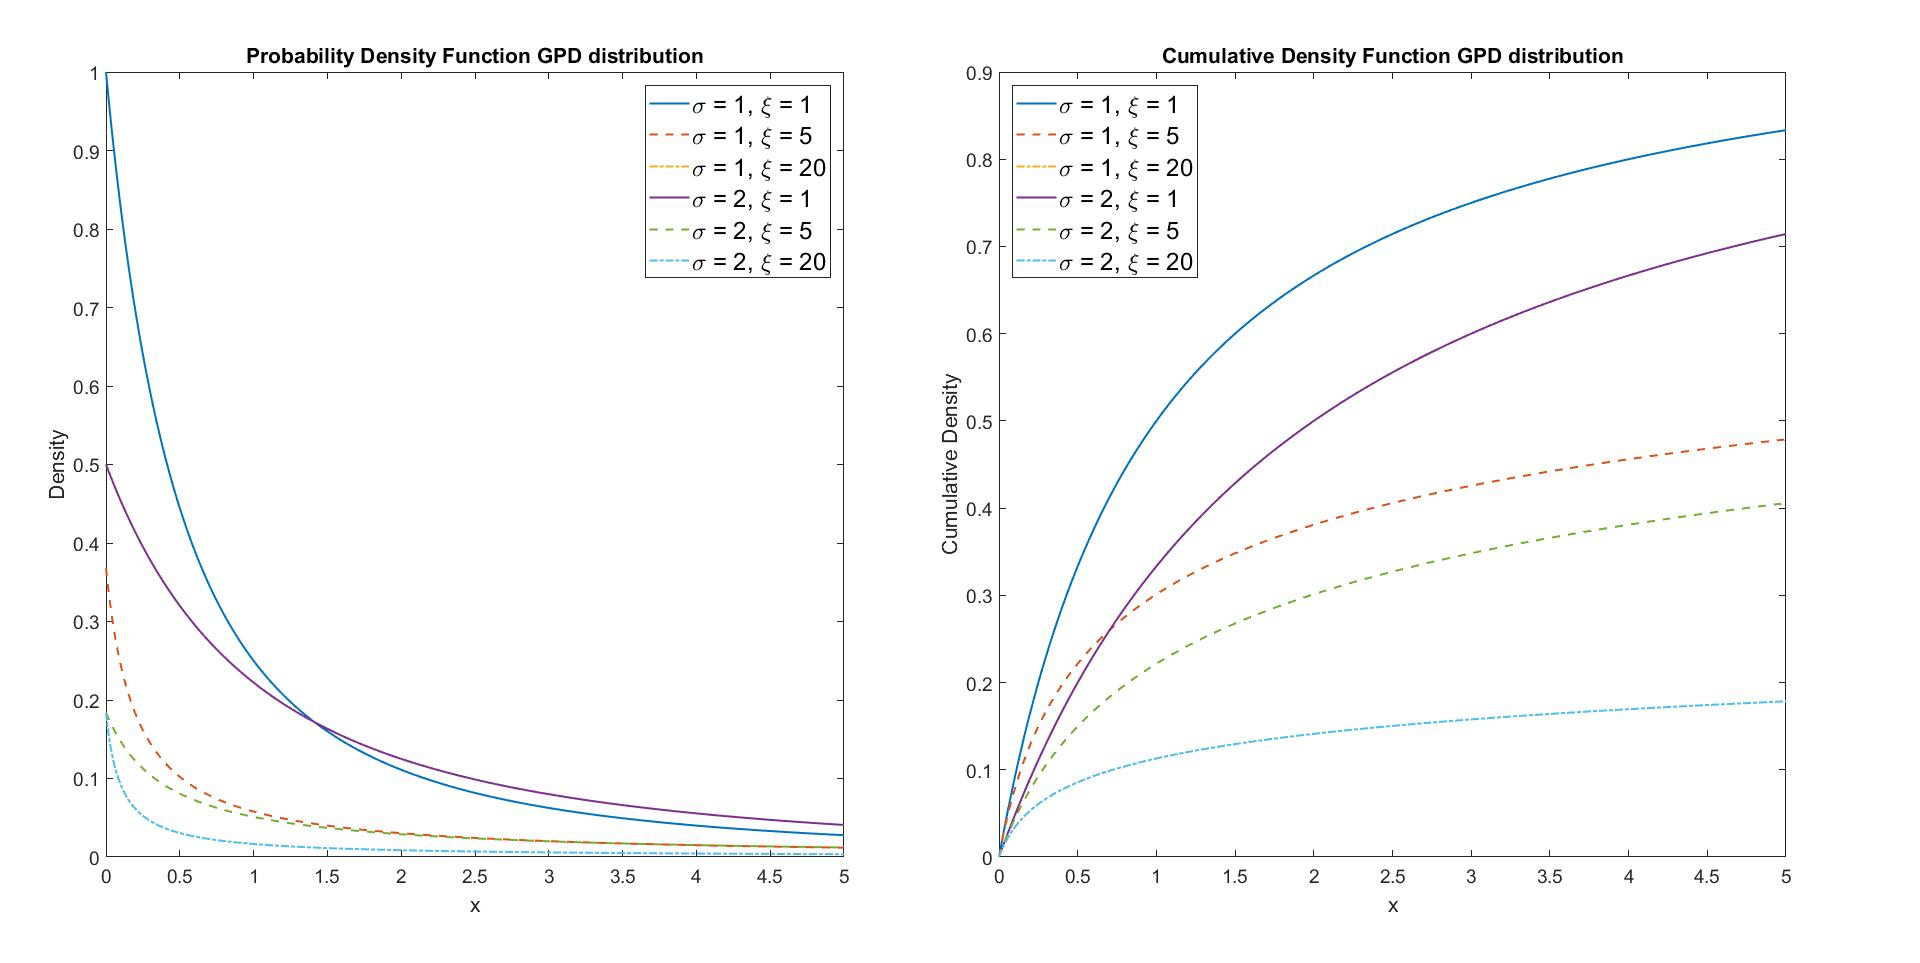
\includegraphics[height=7.8cm, width=\linewidth]{Figures/gpd.jpg} 
\caption{The PDF and CDF for three different values of $\xi$ and two different values for $\sigma$ and setting $\mu=0$.}
\label{fig:gpd}
\end{figure}

Using the rules for probabilities for a random variable $X$ and threshold $u$ such that $x \geq u$,

\begin{equation}
\begin{split}
    \bar{F}(x) &= P(X>u)P(X>x|X>u)\\
    & =\bar{F}(u)P(X-u>x-u|X>u)\\
    & \approx\bar{F}(u)G_{\mu, \sigma, \xi}(x-u)\\
    & \approx\bar{F}(u)(1 + \xi\frac{x-u}{\sigma})^{-\frac{1}{\xi}},
\end{split}
\end{equation}

\noindent where we used the general assumption that $\mu=0$. An estimator for the tail probabilities can then be constructed as proposed by \citeA{smith1987estimating}. There are multiple estimation techniques for obtaining the estimated parameters of the GPD model, for example maximum likelihood or probability-weighted moments. Given that we obtained the estimators for the scale and shape parameters $\hat{\sigma}$ and $\hat{\xi}$ by fitting the GPD to excess losses over threshold $u$ and using the empirical estimator $\frac{k}{N}$ for $\bar{F}(u)$ with $k$, the number of observations exceeding the threshold $u$, this results in the following estimator:

\begin{equation}
    \hat{\bar{F}}(x)=\frac{k}{N}(1 + \hat{\xi}\frac{x-u}{\hat{\sigma}})^{-\frac{1}{\hat{\xi}}}.
    \label{eq:smith}
\end{equation}

As the VaR is just a quantile of the distribution, it can be obtained by inverting the CDF. Applying this to the estimator of the CDF of the excess losses, we derive the estimator for the VaR, the $(1-p_n)$ quantile of $X$ as

\begin{equation}
    \widehat{VaR}_{p_n}=F^{-1}(1-p_n)=u + \frac{\hat{\sigma}}{\hat{\xi}}\left(\left(\frac{k}{N(1-p_n)}\right)^{\hat{\xi}} - 1\right).
    \label{eq:varpotiid}
\end{equation}

We assumed the observations to be of a heavy-tailed distribution or equivalently $\xi>0$. Therefore, the distribution of the observations is in the maximum domain of attraction of the Fr\'echet distribution. Hence, the tail of the distribution is of the form 
\begin{equation}
    \bar{F}(x)=L\left(x\right)x^{-\frac{1}{\xi}},
    \label{eq:power}
\end{equation}
for a slowly varying function $L$. The decay of the tails is a power function in which the rate of decay, denoted by $\frac{1}{\xi}$, is often referred to as the tail index of the distribution. Another conventional method for estimating $\xi$, which utilizes the heavy-tailed distribution, is the Hill estimator, proposed by \citeA{hill1975simple}. The formula for the Hill estimator is given by

\begin{equation}
    \hat{\xi}^{(H)}_{k, N} = \left(\frac{1}{k}\sum^{k}_{j=N-k+1}\ln{X_{j,N}-\ln{X_{k,N}}}\right),
    \label{eq:hillest}
\end{equation}
where $X_{j,N}$ is the $j$-th element in the order statistics $X_{1,N}\leq \dots \leq X_{N,N}$. The difficulty in using the Hill estimator lies in choosing the threshold $u$ and consequently $k$, as it needs to hold that $u \rightarrow \infty$ and $\frac{u}{N} \rightarrow 0$ as $N \rightarrow \infty$. Often, the choice for $u$ is based on the analysis of the so-called Hill plots. There, the estimates of $\xi$ are plotted against the different values for $k$, and the value for $u$ is chosen whenever the estimations become stable. This method has obvious drawbacks with most importantly that it is difficult to implement in an automated way. Hence, a statistical or data-driven selection criterion is needed. \citeA{danielsson2016tail}, recently proposed a selection method that minimizes the maximum distance between the fitted Pareto type tail and the observed quantile.\\

It is common to replace the slowly varying function $L$ in \eqref{eq:power} by a constant $C$, when limiting the observations only to large values.
\begin{equation}
    \bar{F}(x)=Cx^{-\frac{1}{\xi}}, \quad x \geq u > 0,
\end{equation}
for the high threshold $u$. As $\xi$ can be estimated by the Hill estimator \eqref{eq:hillest}, it remains to estimate $C$. Since it holds that $C=u^{\frac{1}{\xi}\bar{F}\left(u\right)}$, substituting again the empirical estimator $\frac{k}{N}$ for $\bar{F}\left(u\right)$ gives the standard form of the Hill tail estimator

\begin{equation}
    \hat{\bar{F}}(x) = \frac{k}{N}\left(\frac{x}{u}\right)^{-\frac{1}{\hat{\xi}^{(H)}}}.
\label{eq:estpotdist}
\end{equation}

\noindent Consequently, the VaR estimator is derived by inverting equation \eqref{eq:estpotdist}

\begin{equation}
        \widehat{VaR}_{p_{n}} &=u\left(\frac{k}{N\left(1-p_n\right)}\right)^{\hat{\xi}^{(H)}_{k,N}}.
        \label{eq:varestpot}
\end{equation}
The limiting distribution of a range of estimators has been thoroughly researched mostly in the IID case, notably by \citeA{dekkers1989moment} and \citeA{de1993estimation}. It is demonstrated that the limiting distribution converges to the normal distribution

\begin{equation}
    \frac{\sqrt{k}}{\log{\left(\frac{k}{Np_n}\right)}}\left(\frac{\widehat{VaR}_{p_n}}{VaR_{p_n}}-1\right)\xrightarrow{\text{d}}\mathcal{N}\left(\lambda, \sigma^2\right) \quad \text{as} \quad N\rightarrow\infty.
\end{equation}
Whenever the data is no longer IID and serial dependence is relevant, the estimator still holds if the serial dependence is weak. \citeA{drees2003extreme} demonstrates that the asymptotic variance is different and usually higher under serial dependence. 

\subsection{Simulation Setup}
The simulation uses a general framework similar to the application. The goal of the simulation setup is to generate multiple scenarios in which the level of autocorrelation, volatility clustering and tail dependence between two series are controlled with a single model. First, the model is explained in steps, then each component is explained in more detail. All the components are then combined into a single model, and how and which parameters will be tuned is discussed at the end.\\

First, the returns of two different series are simulated using an Autoregresive-Moving-Average (ARMA) model of which the innovations are generated by a Generalized Autoregressive Conditional Heteroskedasticity (GARCH) model. The parameters of the ARMA-GARCH model of each series are set independently. The ARMA structure will be the main contributor for generating serially dependent data. The serial dependence can be controlled by both the AR and MA term. The AR term enables the direct incorporation of the dependence of the lagged observations to the current observations. The MA term models the dependence between observations indirectly via the unobserved shocks. By simulating the innovations with a GARCH process instead of a white noise process, the level of volatility clustering within the simulated data can be controlled. The process linking the variance and the innovations, denoted as the GARCH innovations for simplicity, is assumed as a white noise process following the standard normal distribution. Nevertheless, the cross-sectional dependence between the two GARCH innovation processes will be simulated using a Clayton copula. Finally, the simulated portfolio is obtained as a weighted average of the two simulated series as follows, $ X_t = wX_{t,1} + \left(1-w\right)X_{t,2}$.\\

The ARMA(1,1)-GARCH(1,1) model used for each series $j=1,2$ is defined by
\begin{equation}
    \begin{split}
        X_{t,j} &= c_j + \varepsilon_{t,j} + \phi_jX_{t-1,j} + \theta_j\varepsilon_{t-1,j},\\
        \varepsilon_{t,j} &= \sigma_{t,j}z_{t,j}, \\
        \sigma^2_{t,j} &= \omega_j + \alpha_j\varepsilon_{t-1,j}^2 + \beta_j\sigma_{t-1,j}^2, \\
        z_{t,j} &\sim \mathcal{N}\left(0, 1\right),\\
    \end{split}
    \label{eq:armagarchdef}
\end{equation}
and where the copula of $\left(Z_{t,1},Z_{t,2}\right)$ follows the Clayton copula. The conditional variance is denoted by $\sigma^2_t$ and the parameters $\phi_i$, $\theta_i$, $\alpha_i$ and $\beta_i$ are the coefficients of the AR, MA, innovations, and conditional variance terms respectively.\\

Before proceeding to the implementation of the Clayton copula, a general definition of a copula is given as follows: 


\begin{mydef}
A $d$-dimensional copula is a joint cumulative distribution function on $\left[0, 1\right]^d$ with standard uniform marginal distributions.
\end{mydef}

\begin{thm}{\textbf{(Sklar)}}
    Let $F$ be a joint distribution with marginals $F_1,\dots,F_d$. Then there exists a copula $C(x_1,\dots,x_d)$ such that $F(x_1,\dots,x_d)=C(F_1(x_1),\dots,F_d(x_d))$. Conversely, if $C$ is a copula and $F_1,\dots,F_d$ are univariate distributions, then $F$ is a joint distribution with marginals $F_1,\dots,F_d$.
\end{thm}

The bivariate-Clayton copula is an Archimedean copula that allows non-zero level of lower tail dependency between two series. This tail dependency lies in the negative tail, corresponding to extreme losses, and the advantage of the Clayton copula is that the level of dependence can be set by a single parameter, often denoted as $\theta$. The bivariate Clayton copula is given by

\begin{equation}
    C_\theta^{Cl}\left(u_1,u_2\right) = \left(u_1^{-\theta} + u_2^{-\theta} - 1\right)^{-\frac{1}{\theta}} \quad for \quad 0<\theta<\infty.
\end{equation}
Whenever $\theta \to 0$, we approach the independence copula, and when $\theta \to \infty$, we approach full dependency.\\

To combine all the different components in the simulation model, we derived the following algorithm to obtain a single set of simulated data.

\newtheorem{myalgo}{Algorithm}
\begin{myalgo}{\textbf{(Data Generating Process)}}
    \quad
    \begin{enumerate}
        \item Generate two uniformly distributed series from the Clayton copula. Draw two independent uniform random variables $\left(U_{t,1},V_{t,2}\right)$ and set
            \begin{equation}                U_{t,2}=\left[U_{t,1}^{-\theta^{Cl}}\left(v_{2}^{-\frac{\theta^{Cl}}{\left(1+\theta^{Cl}\right)}}-1\right)+1\right]^{-\frac{1}{\theta^{Cl}}}.
            \end{equation}
        \item Convert the $\left(U_{t,1},U_{t,2}\right)$ to standard normal marginals using the inverse of the standard normal CDF
        \begin{equation}
            Z_{t,1} = \Phi^{-1}(U_{t,1}) \quad \text{and} \quad Z_{t,2} = \Phi^{-1}(U_{t,2}).
        \end{equation}
        The simulated standard normal variables $Z_{t,1}$ and $Z_{t,2}$ have lower tail dependency but are both IID series.
        \item Using $\left(Z_{t,1},Z_{t,2}\right)$ to simulate two series from the ARMA(1,1)-GARCH(1,1) model for $j=1,2$:
        \begin{equation}
            \begin{split}
                X_{t,j} &= c_{j} + \varepsilon_{t,j} + \phi_{j}X_{t-1,j} + \theta_{j}\varepsilon_{t-1,j},\\ \varepsilon_{t,j} &= \sigma_{t,j}z_{t,j}\\
                \sigma^2_{t,j} &= \omega_j + \alpha_{j}\varepsilon_{t-1,j}^2 + \beta_{j}\sigma_{t-1,j}^2.
            \end{split}
            \label{eq:simarmagarchdef}
        \end{equation}
        \item Obtain the simulated time series by calculating the weighted average
        \begin{equation}
            X_t = wX_{t,1} + \left(1-w\right)X_{t,2}.
        \end{equation}
    \end{enumerate}
\end{myalgo}

For every specification of the parameters, one sample with sample size $1,000,000$ is obtained to calculate the true VaR and $1,000$ samples with sample size $2,000$ are generated for comparing the two methods to estimate the VaR. Every sample will use a burn-in sample size of $1,000$ data points. The true VaR is then estimated as the empirical quantile from the large sample.\\

The set of models are divided into two groups: the first group depends only on one ARMA-GARCH model by setting $w=1$ and $z_{t,1}\sim \mathcal{N}\left(0, 1\right)$, the second group uses the Clayton copula to introduce tail dependency and the two time series are combined by setting $w=0.5$.

\subsection{Simulation Evaluation}
In the simulation application it is possible to obtain the true VaR and hence, the VaR estimates are evaluated by calculating the root mean squared error (RMSE) and root mean squared percentage error (RMSPE). After obtaining $m=1,000$ VaR estimates per simulation model described in section 4.4, the RMSE and RMSPE can be calculated as

\begin{equation}
    RMSE = \sqrt{\frac{\sum^m_{i=1}\left(\widehat{VaR}_{p_n} - VaR_{p_n}\right)^2}{m}},
    \label{eq:rmse}
\end{equation}

\begin{equation}
    RMSPE = \sqrt{\frac{\sum^m_{i=1}\left(\frac{\widehat{VaR}_{p_n}}{VaR_{p_n}} - 1\right)^2}{m}}.
    \label{eq:mape}
\end{equation}
 \\
For both the POT and BM method, the RMSE is calculated using same true VaR. For a given specification of parameters, we can directly compare the performance of the two methods using RMSE. However, since the scale of the true VaR will differ across different specifications of parameters, it is not possible to make a comparison across different specifications of parameters using RMSE. The RMSPE is based on the percentage deviation and will therefore be used to compare the two methods at different parameter specifications. 

\subsection{Application}
In the financial application, the VaR is estimated on a stock-bond portfolio using both methods. Since the underlying data generating process is unknown, we can not evaluate the VaR estimates by comparing it to the true VaR. The VaR estimates are now evaluated using the binomial method as demonstrated by \citeA{christoffersen1998evaluating}. The binomial method is based on the unconditional coverage of the risk measure. The unconditional coverage can be seen as the empirical probability of exceeding the estimated VaR, $a^*=\frac{x}{N}$, with $x$ the number of observations exceeding the VaR estimate. By definition, the unconditional coverage should equal the confidence level of the VaR. Assume the confidence level $p_n$, then the probability of observing $x$ exceptions in a testing sample of sample size $W$ should equal the binomial pdf under the null hypothesis \begin{equation}
    Pr\left(x\right) = {W\choose x}p_n^x\left(1-p_n\right)^{W-x}.
\end{equation}
\noindent A likelihood ratio test statistic is performed to test whether the unconditional coverage is equal to $p_n$. The test statistic can be calculated by
\begin{equation}
    LR_{uc} = 2\left[\ln{\left(a^{*^x}\left(1-a^*\right)^{W-x}\right)}-\ln{\left(p_n^x\left(1-p_n\right)^{W-x}\right)}\right]\sim \chi^2\left(1\right).
\end{equation}

\newpage
\section{Empirical Data}
\subsection{Preliminary}
The empirical analysis focuses on a diversified portfolio of European markets. We setup a hypothetical portfolio investing $70\%$ in stocks and $30\%$ in bonds. The STOXX Europe 600 index, which holds 600 European companies, is used to represent the European stock market. The index represents large, medium and small capitalisation companies in 17 European countries that, cover approximately 90$\%$ of the free-float market capitalisation of the European stock market. The Barclays Euro Aggregate Treasury Total Return Index is used to represent the European bond market. This bond index contains 372 fixed-income securities from 13 different countries and are weighted by their market value. The data is obtained from Bloomberg Financial Markets and contain daily observations from 1 January, 2000 till 31 December, 2017, which results in 4,550 observations for each index. The index values are converted to daily returns as $r_t = log(I_t/I_{t-1})$ where $I_t$ is the index value at time $t$. Figure \ref{fig:data} illustrates the index levels and returns of the stock index, bond index, and the stock-bond portfolio respectively. 


\begin{figure}[H]
$\begin{array}{rl}
    \multicolumn{2}{c}{\text{\small{(a) STOXX Europe Index}}} \\
    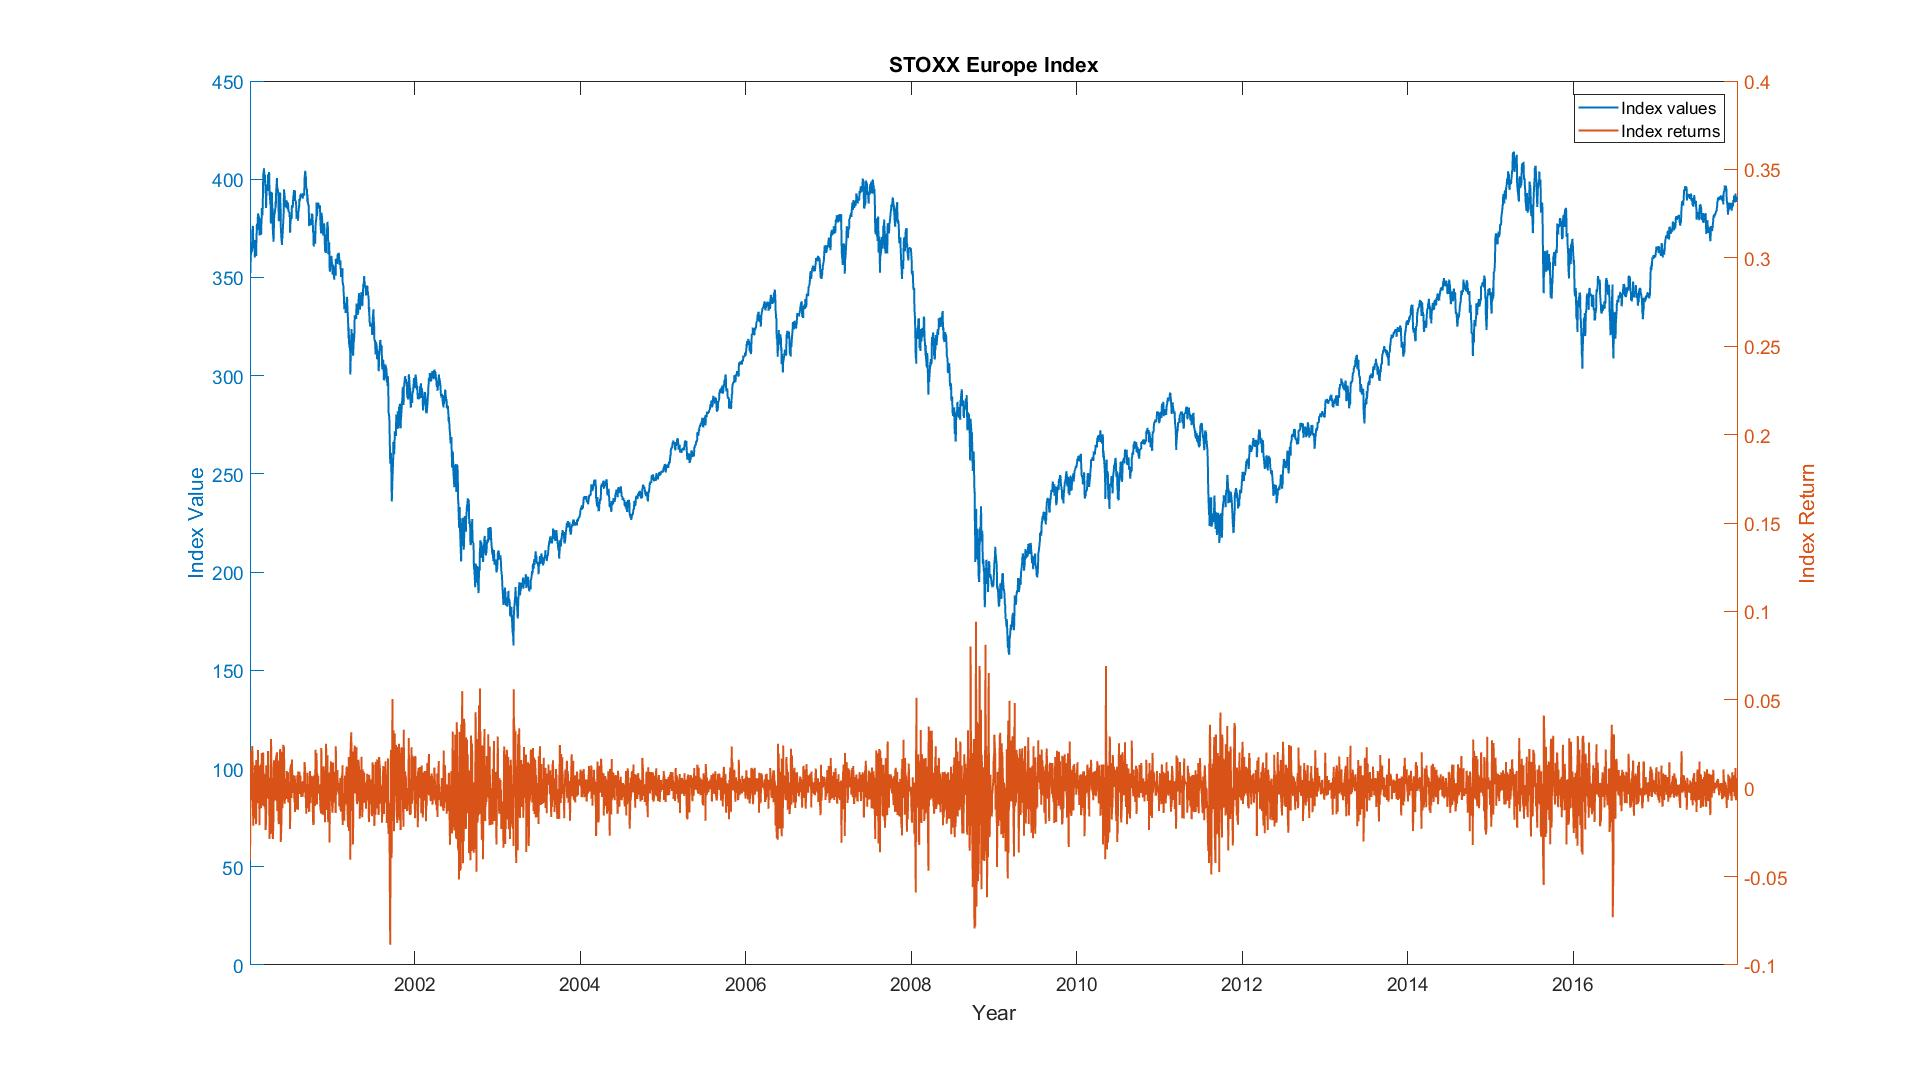
\includegraphics[height=7.25cm, width=1\linewidth]{Figures/stocks.jpg}  \\
    \multicolumn{2}{c}{\text{\small{(b) Barclays Euro Aggregate Treasury Total Return Index}}} \\
    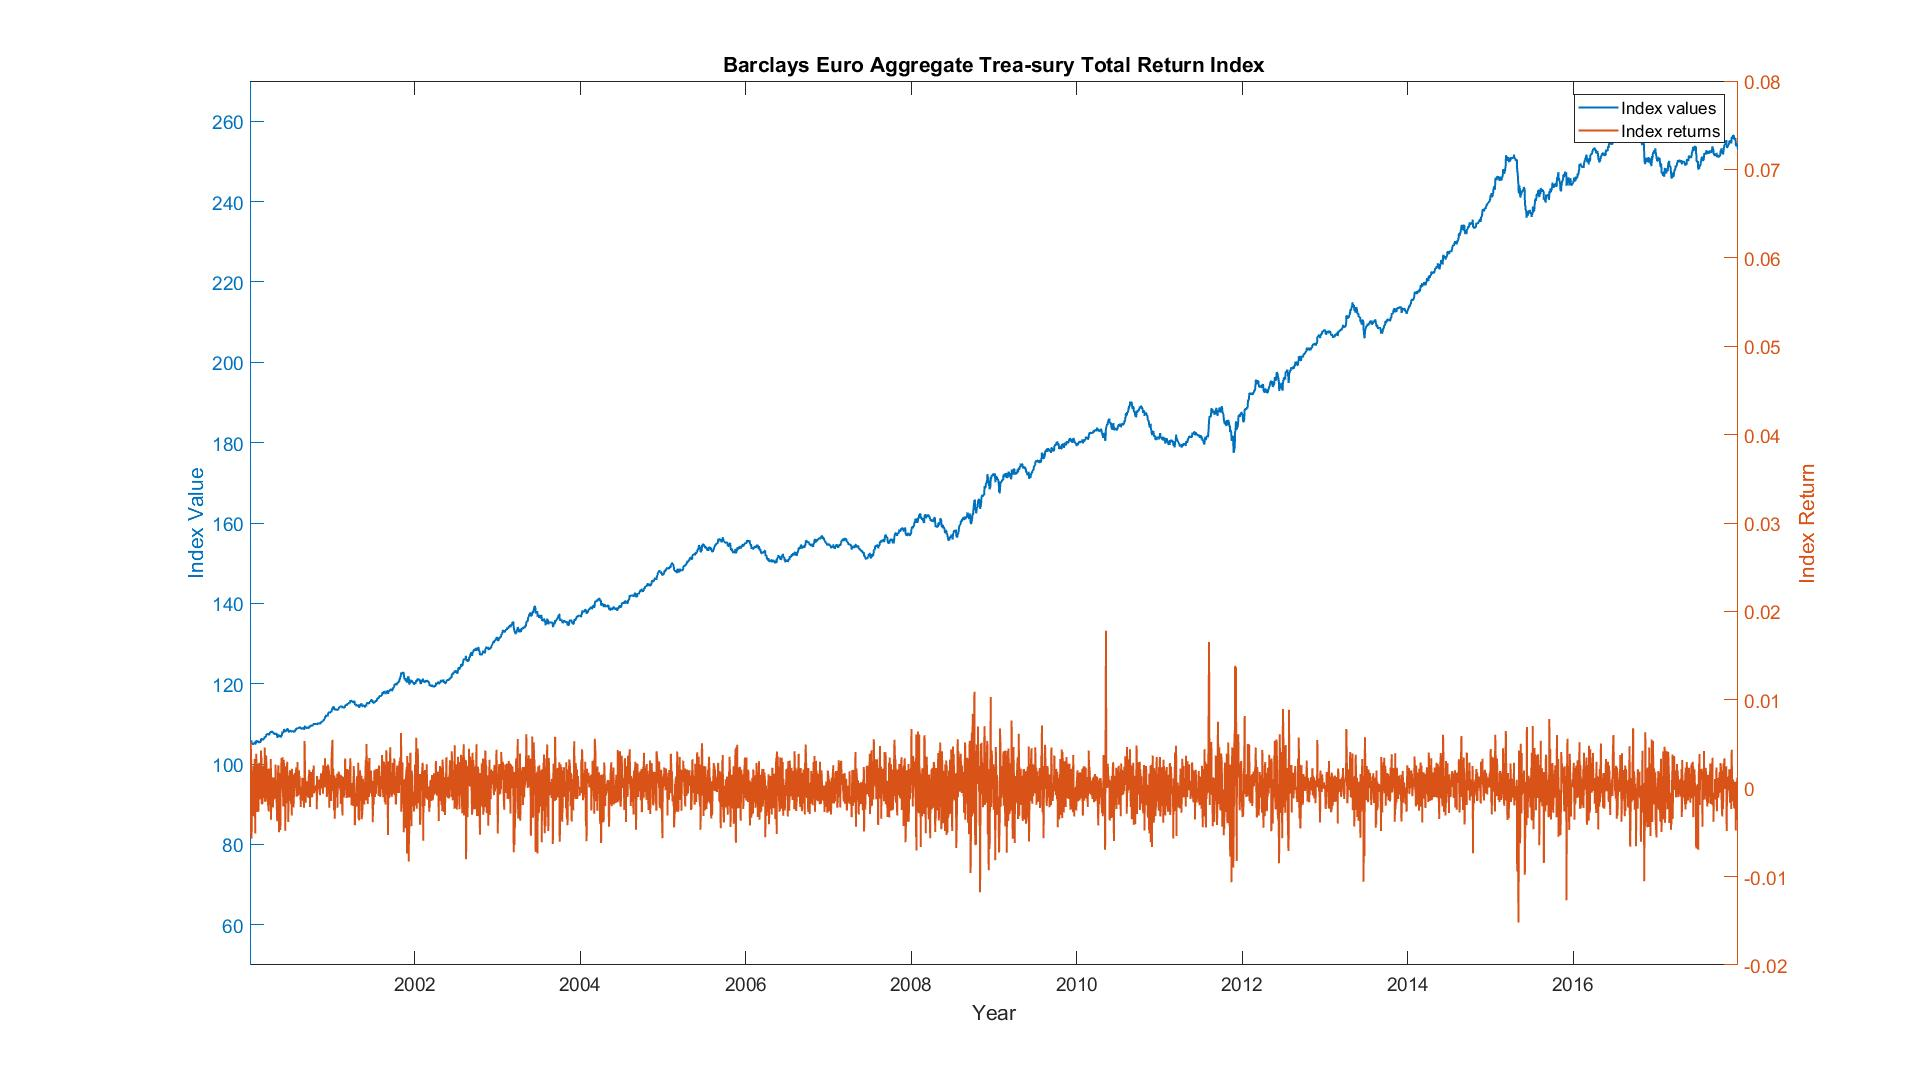
\includegraphics[height=7.25cm, width=1\linewidth]{Figures/bonds.jpg}\\ 
    \multicolumn{2}{c}{\text{\small (c) Portfolio returns with $70\%$ stocks and $30\%$ bonds allocation}} \\
    \multicolumn{2}{c}{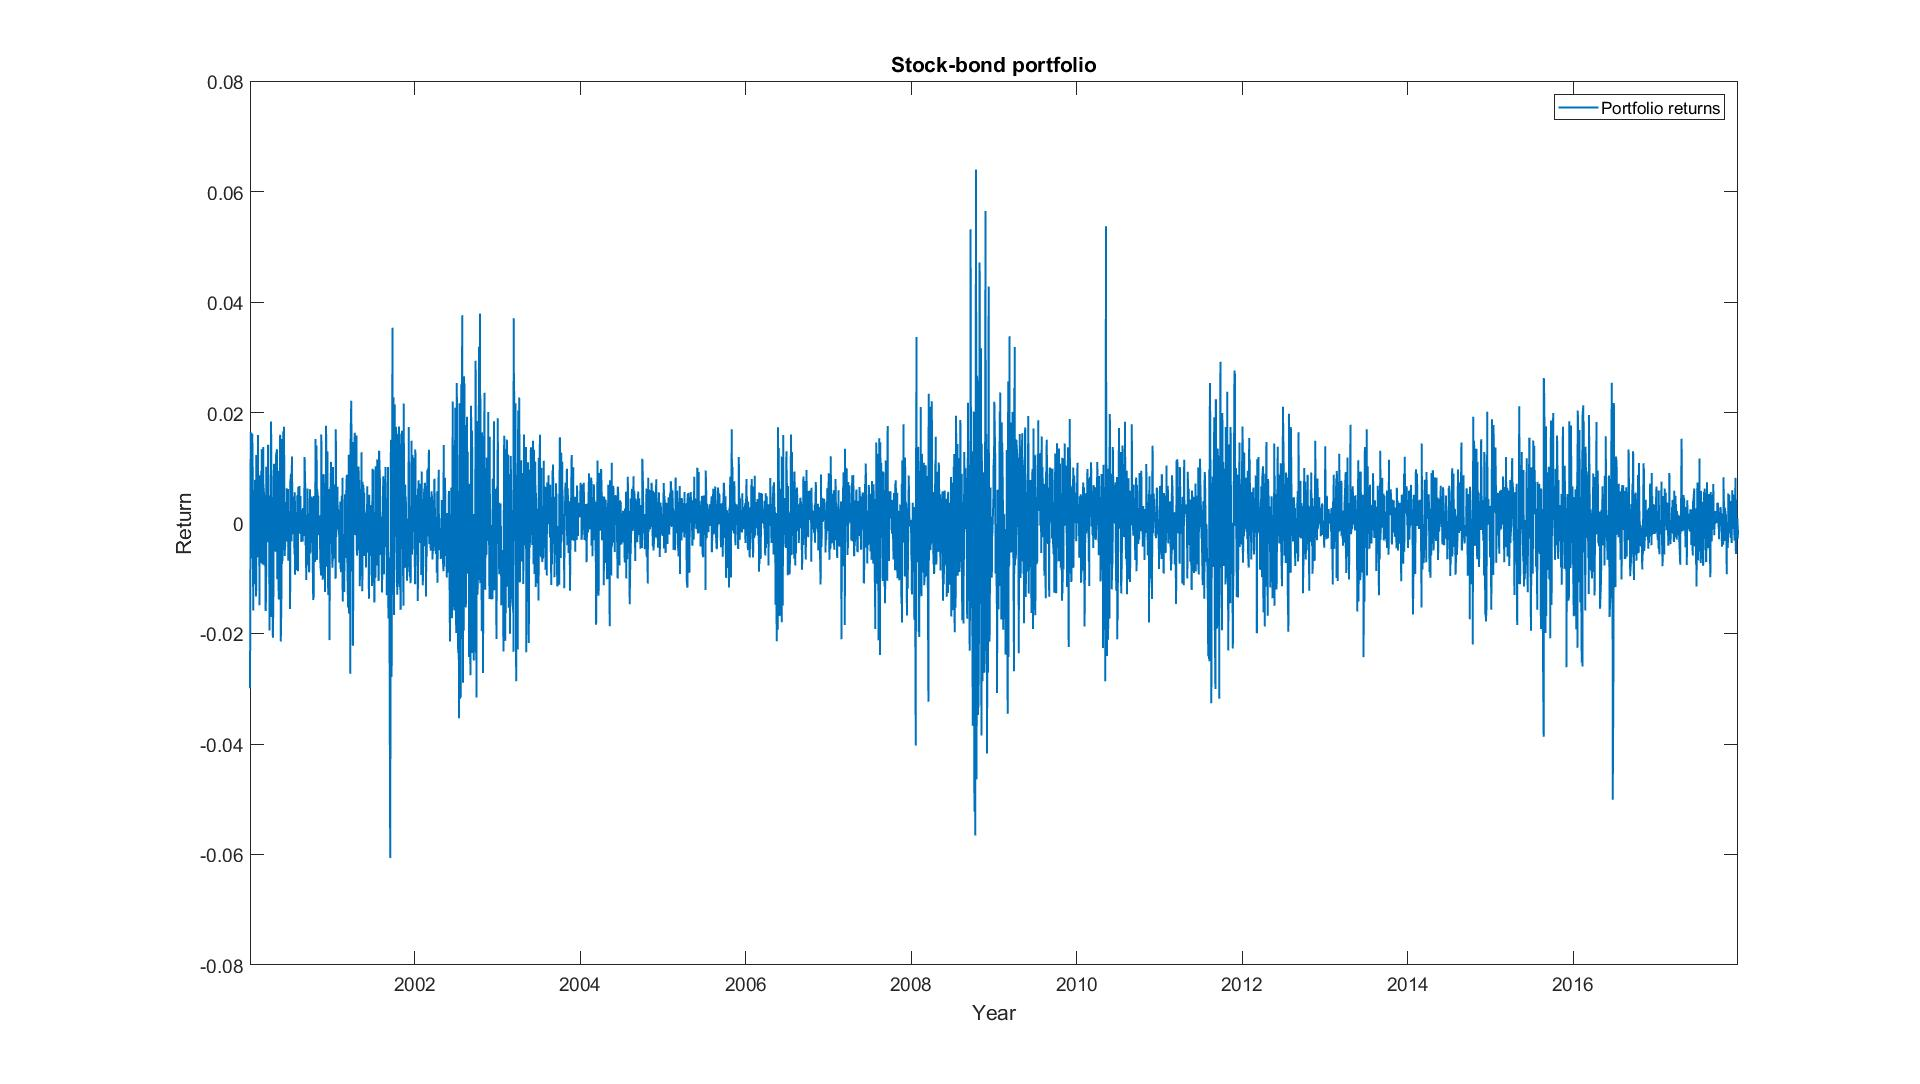
\includegraphics[height=7.25cm, width=1\linewidth]{Figures/portfolio.jpg}} 
\end{array}$
\vspace{-0.8cm}
\captionsetup[figure]{font=small,labelfont=small}
\caption{Index levels and returns for the stock index, the bond index and the portfolio.}
\label{fig:data}
\end{figure}

The period from the beginning of 2000 till the end of 2017 is of interest because it contains two major events: the burst of the dot-com bubble in 2000 and the global financial crisis of 2008. Both events are represented by a large spike in volatility which is more prominent in the stock index than the bond index, as expected. Even though the portfolio is well-diversified with positions in 600 different stocks and 372 fixed-income securities, there is still a clear indication of volatility clustering.

\subsection{Descriptive Statistics}
The statistical properties of the empirical data need to be analysed in further detail. The descriptive statistics are outlined in Table \ref{tab:desstats}. As expected from the difference in nature between stocks and fixed-income securities, the standard deviation of the stock index is almost six times as high as the standard deviation of the bond index. The returns of both indices are well centred around zero, as indicated by the mean and median. For both indices the skewnesses are negative and with kurtosises higher then 3, that of the normal distribution. It is common for financial securities to have more extreme losses than extreme profits as reflected by the negative skewness. The stylised fact of more extreme values than the normal distribution and hence the notion of fatter tails is captured by the high values of kurtosis. Formally, we reject that each series follow a normal distribution by the Jarque-Bera test. As the chosen portfolio is a weighted average between the stock and bond index, the values of the statistical properties lie between those of the stock and bond index.


\begin{table}[H]
\captionsetup{width=.9\textwidth}
\caption{Descriptive statistics of the stock index, bond index, and portfolio returns.} 
\centering
\label{tab:desstats}
\scalebox{0.7}{
\begin{tabular}{l|lllllllllll} \hline \hline
\textbf{Return Series} & \textbf{\# Obs} & \textbf{Min.}    & \textbf{Max.}   & \textbf{Mean} & \textbf{Median}   & \textbf{Std. Dev} & \textbf{Skewness} & \textbf{Kurtosis} & \textbf{Jarque-Bera} \\ \hline
STOXX 600     & 4549   & -0.0886 & 0.0941 & 0.0000 & 0.0003 & 0.0124   & -0.2125  & 8.5901  & 0.0000 \\
Barclays Bond & 4549   & -0.0152 & 0.0178 & 0.0002 & 0.0002 & 0.0023   & -0.1371  & 6.5306  & 0.0000   \\
Portfolio     & 4549   & -0.0606  & 0.0640 & 0.0000 & 0.0002 & 0.0086   & -0.2023  & 8.4798  & 0.0000  \\ \hline \hline
\end{tabular}}
\end{table}\\

The results of the Ljung-Box test can be found in Table \ref{tab:ljungbox}, which provide more in-depth analysis of the serial dependency. Furthermore, Figure \ref{fig:autocorrs} demonstrates autocorrelation and partial autocorrelation plots of the portfolio returns and the squared portfolio returns. The Ljung-Box Q-test indicates that for all returns series, the null hypothesis of independently distributed data can be rejected at a $5\%$ significance level. These results are further supported by the correlation plots of the portfolio returns. For both the autocorrelation and the partial autocorrelation, there are multiple lags with significant correlation, most notably at lags 2, 3, 5, and 6. The correlation plots of the squared portfolio returns exhibit a strong significant autocorrelation. This confirms the presence of volatility clustering.
\newpage

\begin{table}[H]
\captionsetup{width=.9\textwidth}
\caption{Ljung-Box Q-test results.} 
\centering
\label{tab:ljungbox}
\scalebox{0.9}{
\begin{tabular}{l|lll}
\hline \hline
\textbf{Return Series}    & \textbf{Test-statistic} & \textbf{Critical value} & \textbf{\textit{p}-value} \\ \hline
STOXX 600         & 54.02          & 31.41          & 0.0006  \\
Barclays Bond     & 41.39          & 31.41          & 0.0033  \\
Portfolio         & 49.81          & 31.41          & 0.0002  \\
Squared Portfolio & 3940.17        & 31.41          & 0.0000  \\ \hline \hline
\end{tabular}}
\begin{tablenotes}
      \tiny
      \item * Test results are based on significance level $\alpha=5\%$ and degrees of freedom equal to number of lags selected is 20.
\end{tablenotes}
\end{table}


\begin{figure}[H]
$\begin{array}{rl}
    \multicolumn{1}{c}{\text{\small{(a) Serial dependence analysis on the portfolio returns}}} \\
    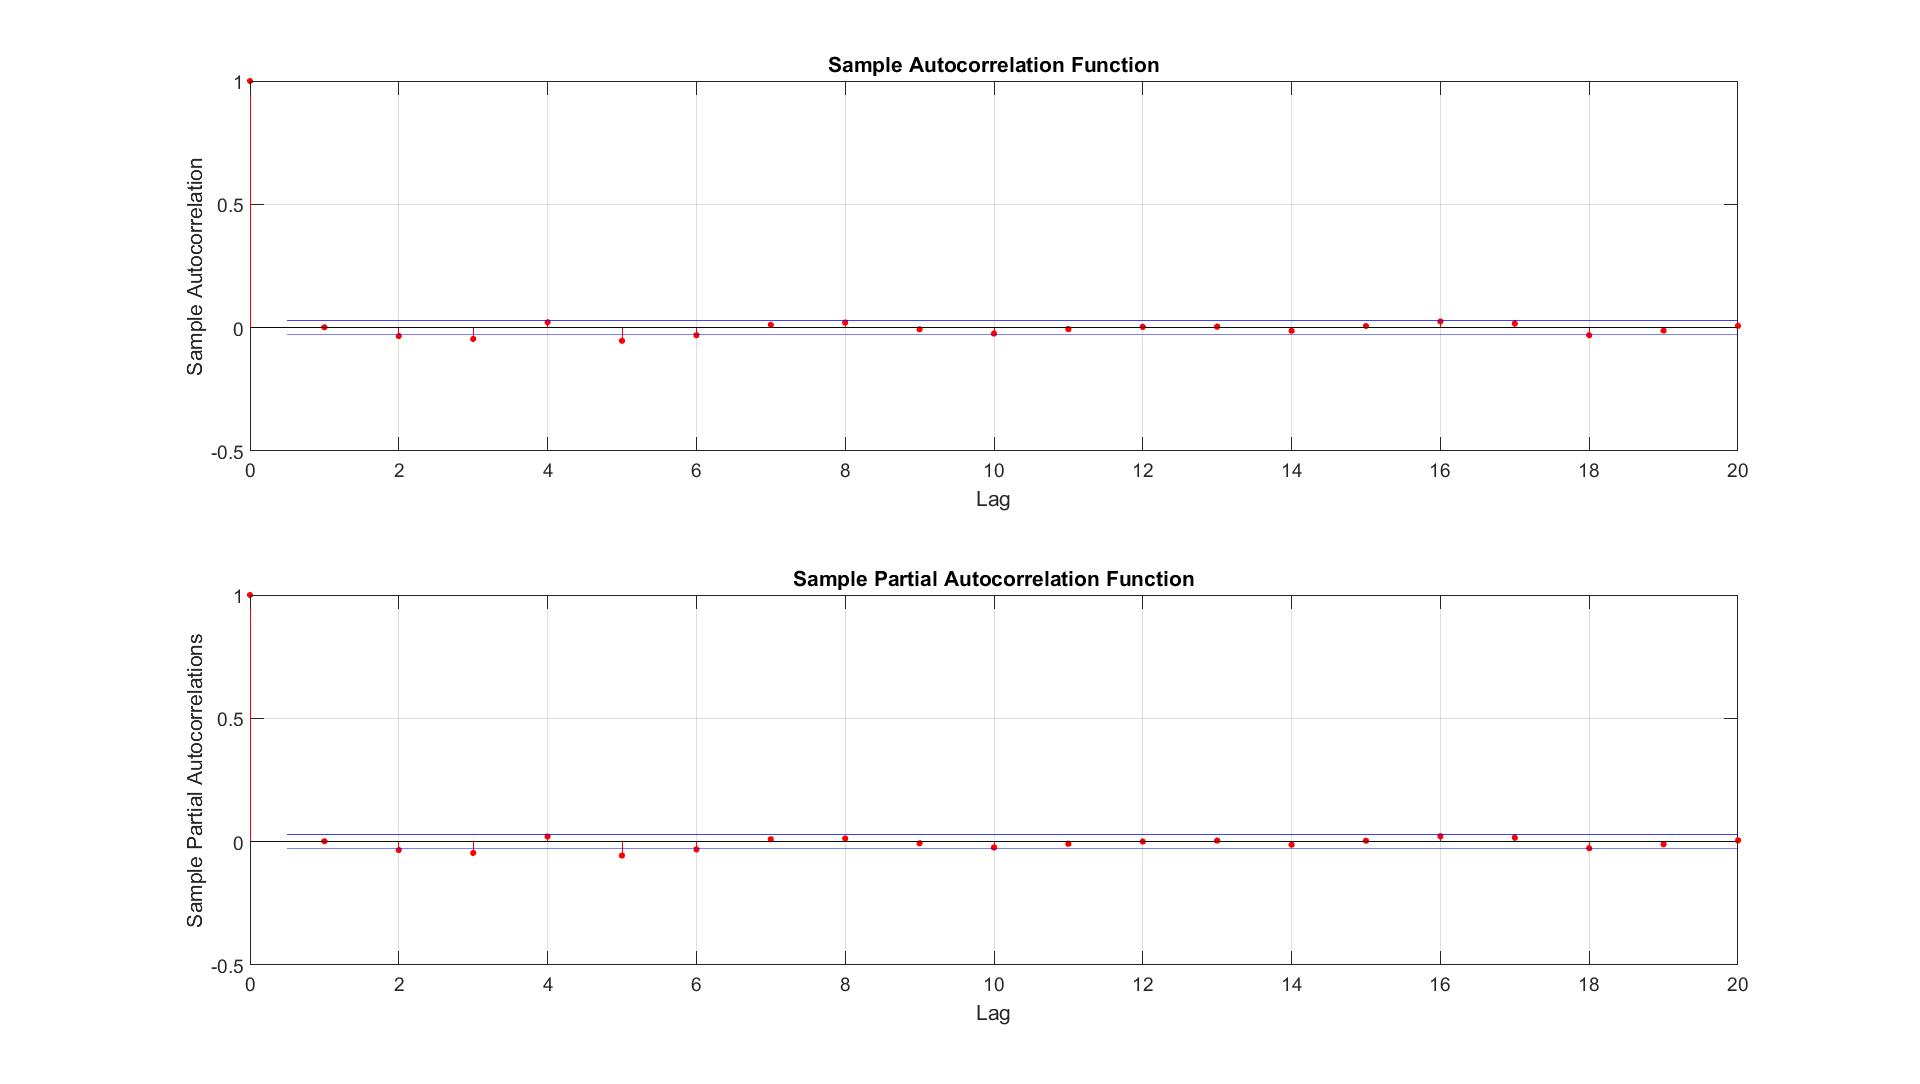
\includegraphics[height=7.8cm, width=1\linewidth]{Figures/portfolio_returns_autocorr.jpg}  \\
    \multicolumn{1}{c}{\text{\small{(b) Serial dependence analysis on the squared portfolio returns}}} \\
    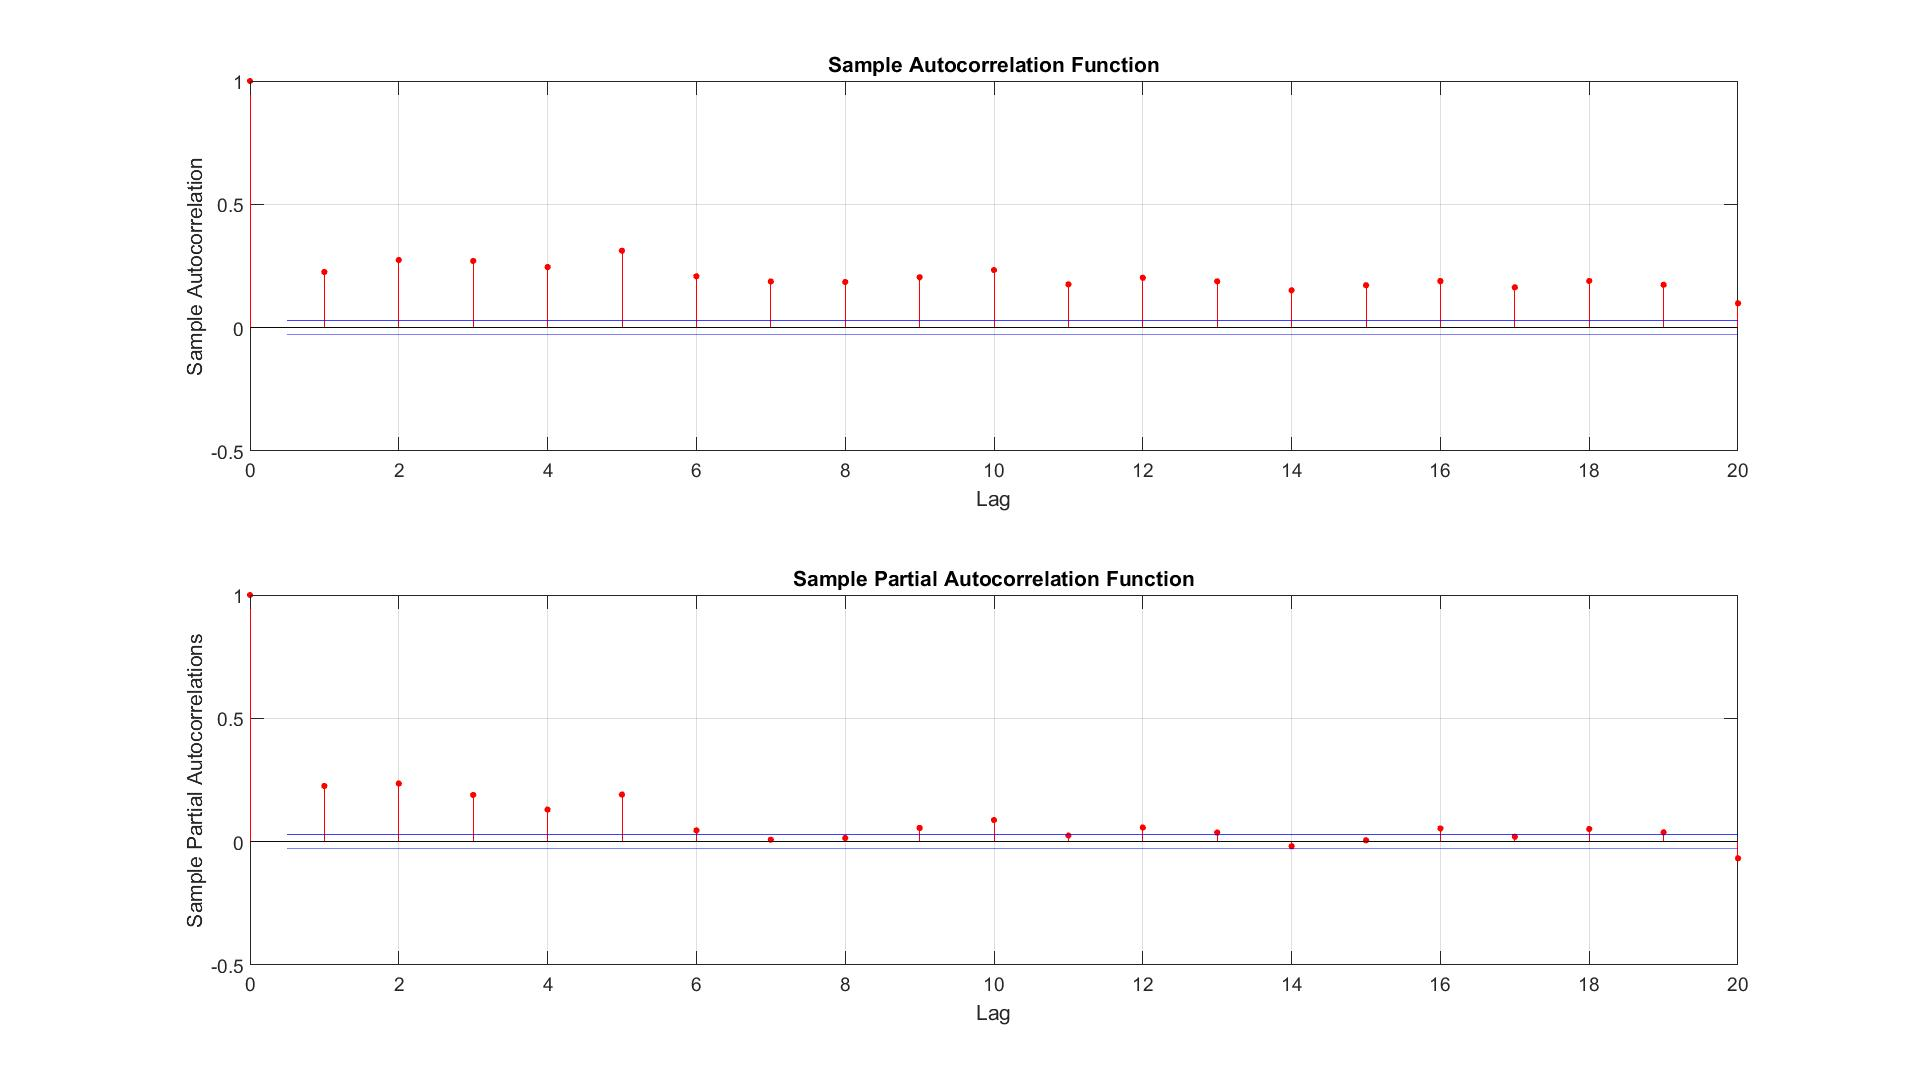
\includegraphics[height=7.8cm, width=1\linewidth]{Figures/squared_portfolio_returns_autocorr.jpg}
\end{array}$
\vspace{-0.8cm}
\captionsetup[figure]{font=small,labelfont=small}
\caption{Sample autocorrelation and partial autocorrelation plots of the realised and squared portfolio returns.}
\label{fig:autocorrs}
\end{figure}

\newpage

\section{Results}
\subsection{Simulation Application}
\begin{comment}
\begin{itemize}
    \item Intro -> first only ARMA then rest
    \item Focus is thus on serial dependence
    \item Result: POT performs better then BM 
    \item Surface plots
\end{itemize}
\end{comment}
The simulation is divided into three groups to assess the performance of the POT and BM method and are discussed in order. With the ARMA model the effect of serial dependence is highlighted. By extending the model with GARCH innovations, we can verify the estimation performance of the POT and BM method in the presence of volatility clustering. In the same way, the impact of cross-sectional dependence in the tail on estimating the VaR is discussed by using the Clayton copula.\\

To analyze the serial dependence, the ARMA model defined by equation \eqref{eq:simarmagarchdef} is used. As the GARCH innovations and the cross-sectional dependence are not considered yet, we set the parameters to $j=1$, $\alpha_j=0$, $\beta_j=0$ and $\omega_j=1$. The innovations follow the Student's t-distribution with 2 degrees of freedom, $z_{t,j}\sim t\left(2\right)$ as this ensures the fat-tails, or equivalently $\xi>0$. The level of serial dependence is controlled via the parameters $\phi$ and $\theta$. We setup a grid with the values for $\phi$ and $\theta$ ranging from $0$ to $0.95$, with step size $0.05$. Hence, this also includes the IID case whenever $\phi=0$ and $\theta=0$. Figure \ref{fig:results_arma_simdata2} displays in increasing order of serial dependence, three randomly chosen simulated time-series. The observed outliers are an confirmation of the fat-tails or $\xi>0$, due to the Student's t distributed innovations.

\begin{figure}[H]
$\begin{array}{rl}
    \multicolumn{1}{c}{\text{\small{(a) Simulated series with $\phi=0.1$ and $\theta=0.1$}}} \\
    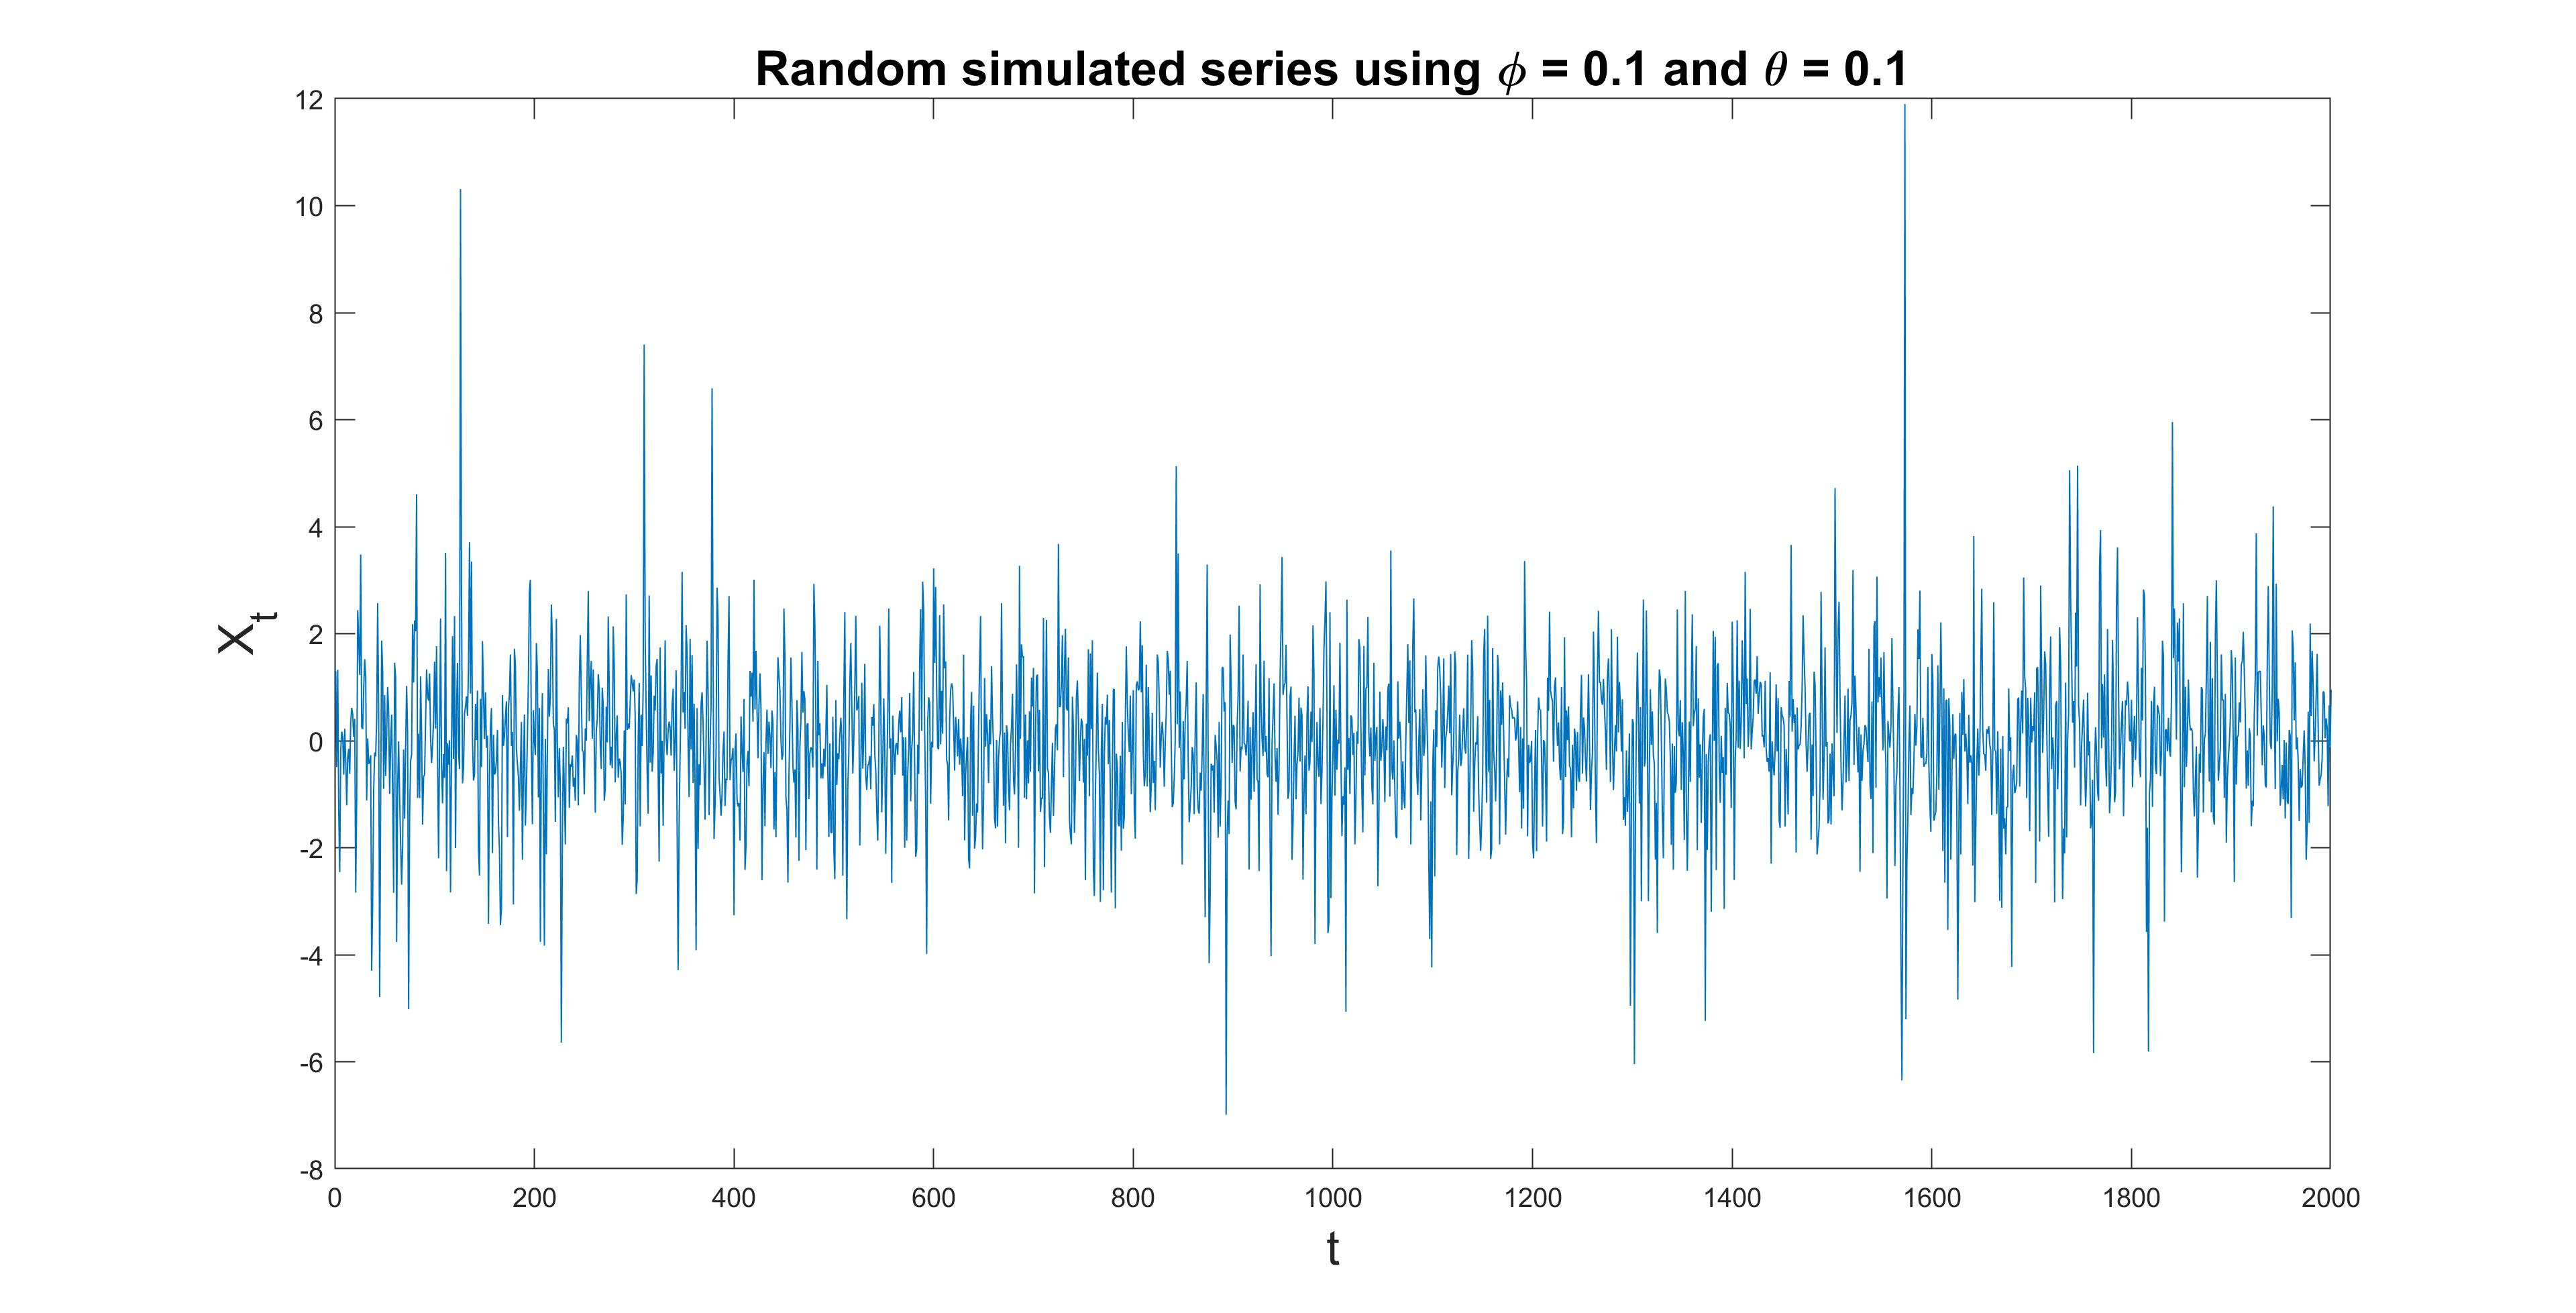
\includegraphics[height=7.25cm, width=1\linewidth]{Figures/results_arma_simdata1.jpg}
\end{array}$
\vspace{-0.8cm}
\captionsetup[figure]{font=small,labelfont=small}
\caption*{}
\label{fig:results_arma_simdata1}
\end{figure}

\begin{figure}[H]
$\begin{array}{rl}
    \multicolumn{2}{c}{\text{\small{(b) Simulated series with $\phi=0.5$ and $\theta=0.5$}}} \\
    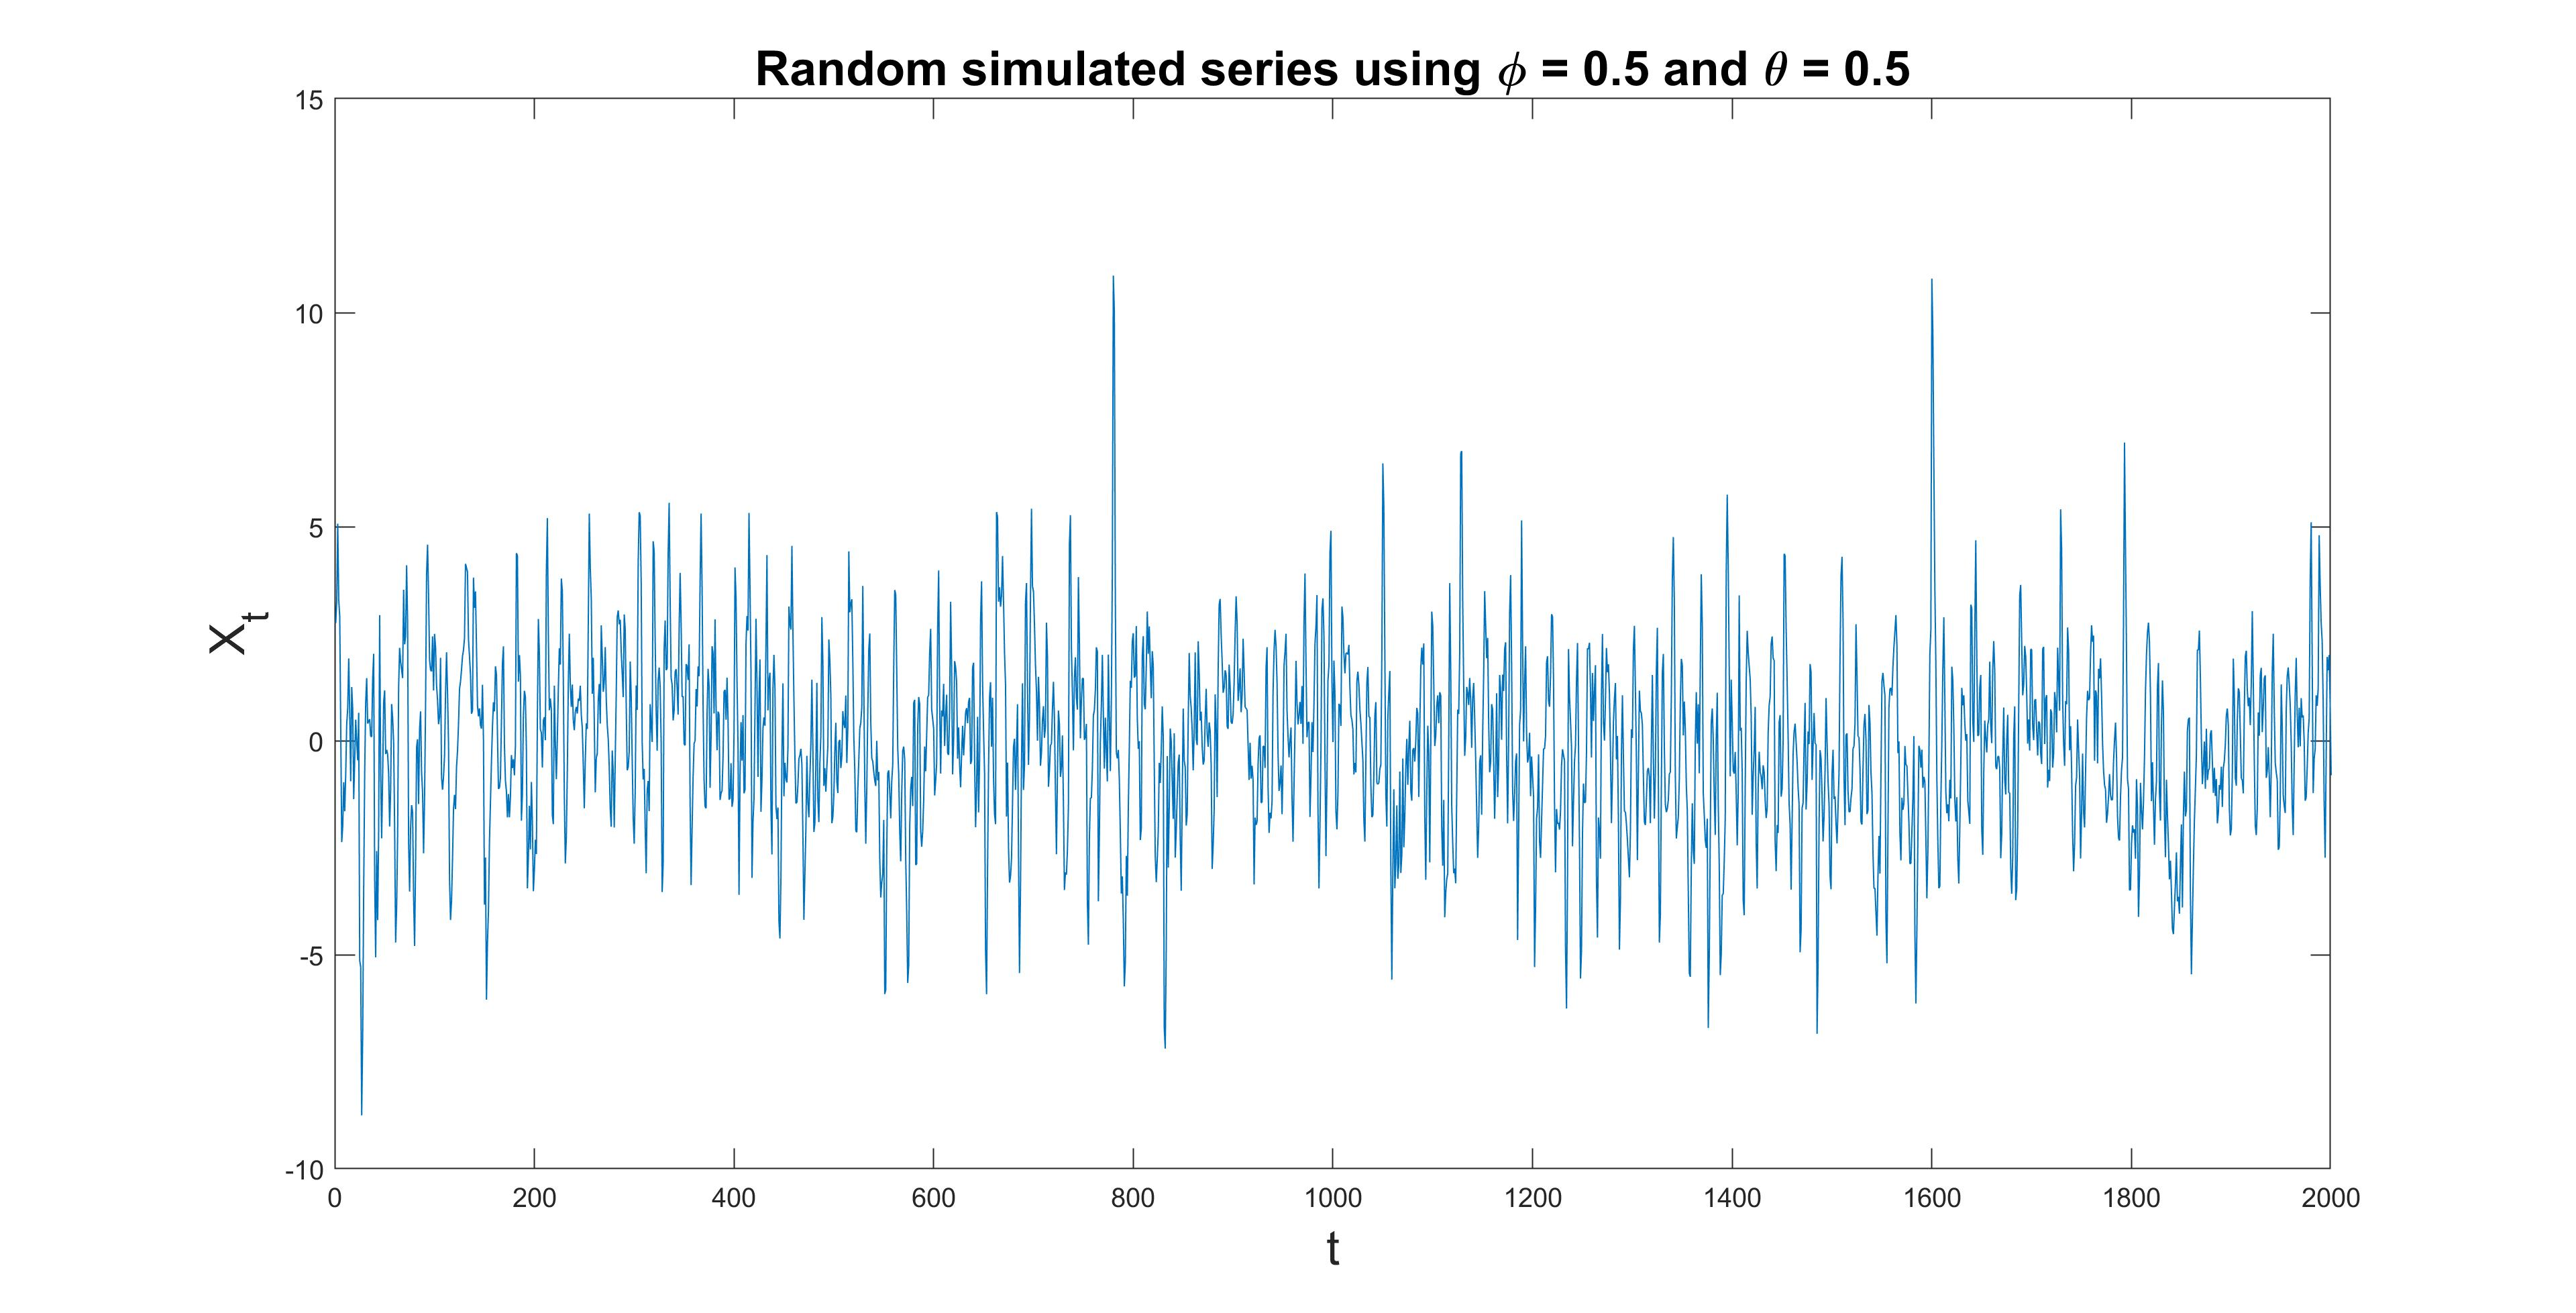
\includegraphics[height=7.25cm, width=1\linewidth]{Figures/results_arma_simdata2.jpg}\\ 
    \multicolumn{2}{c}{\text{\small (c) Simulated series with $\phi=0.9$ and $\theta=0.9$}} \\
    \multicolumn{2}{c}{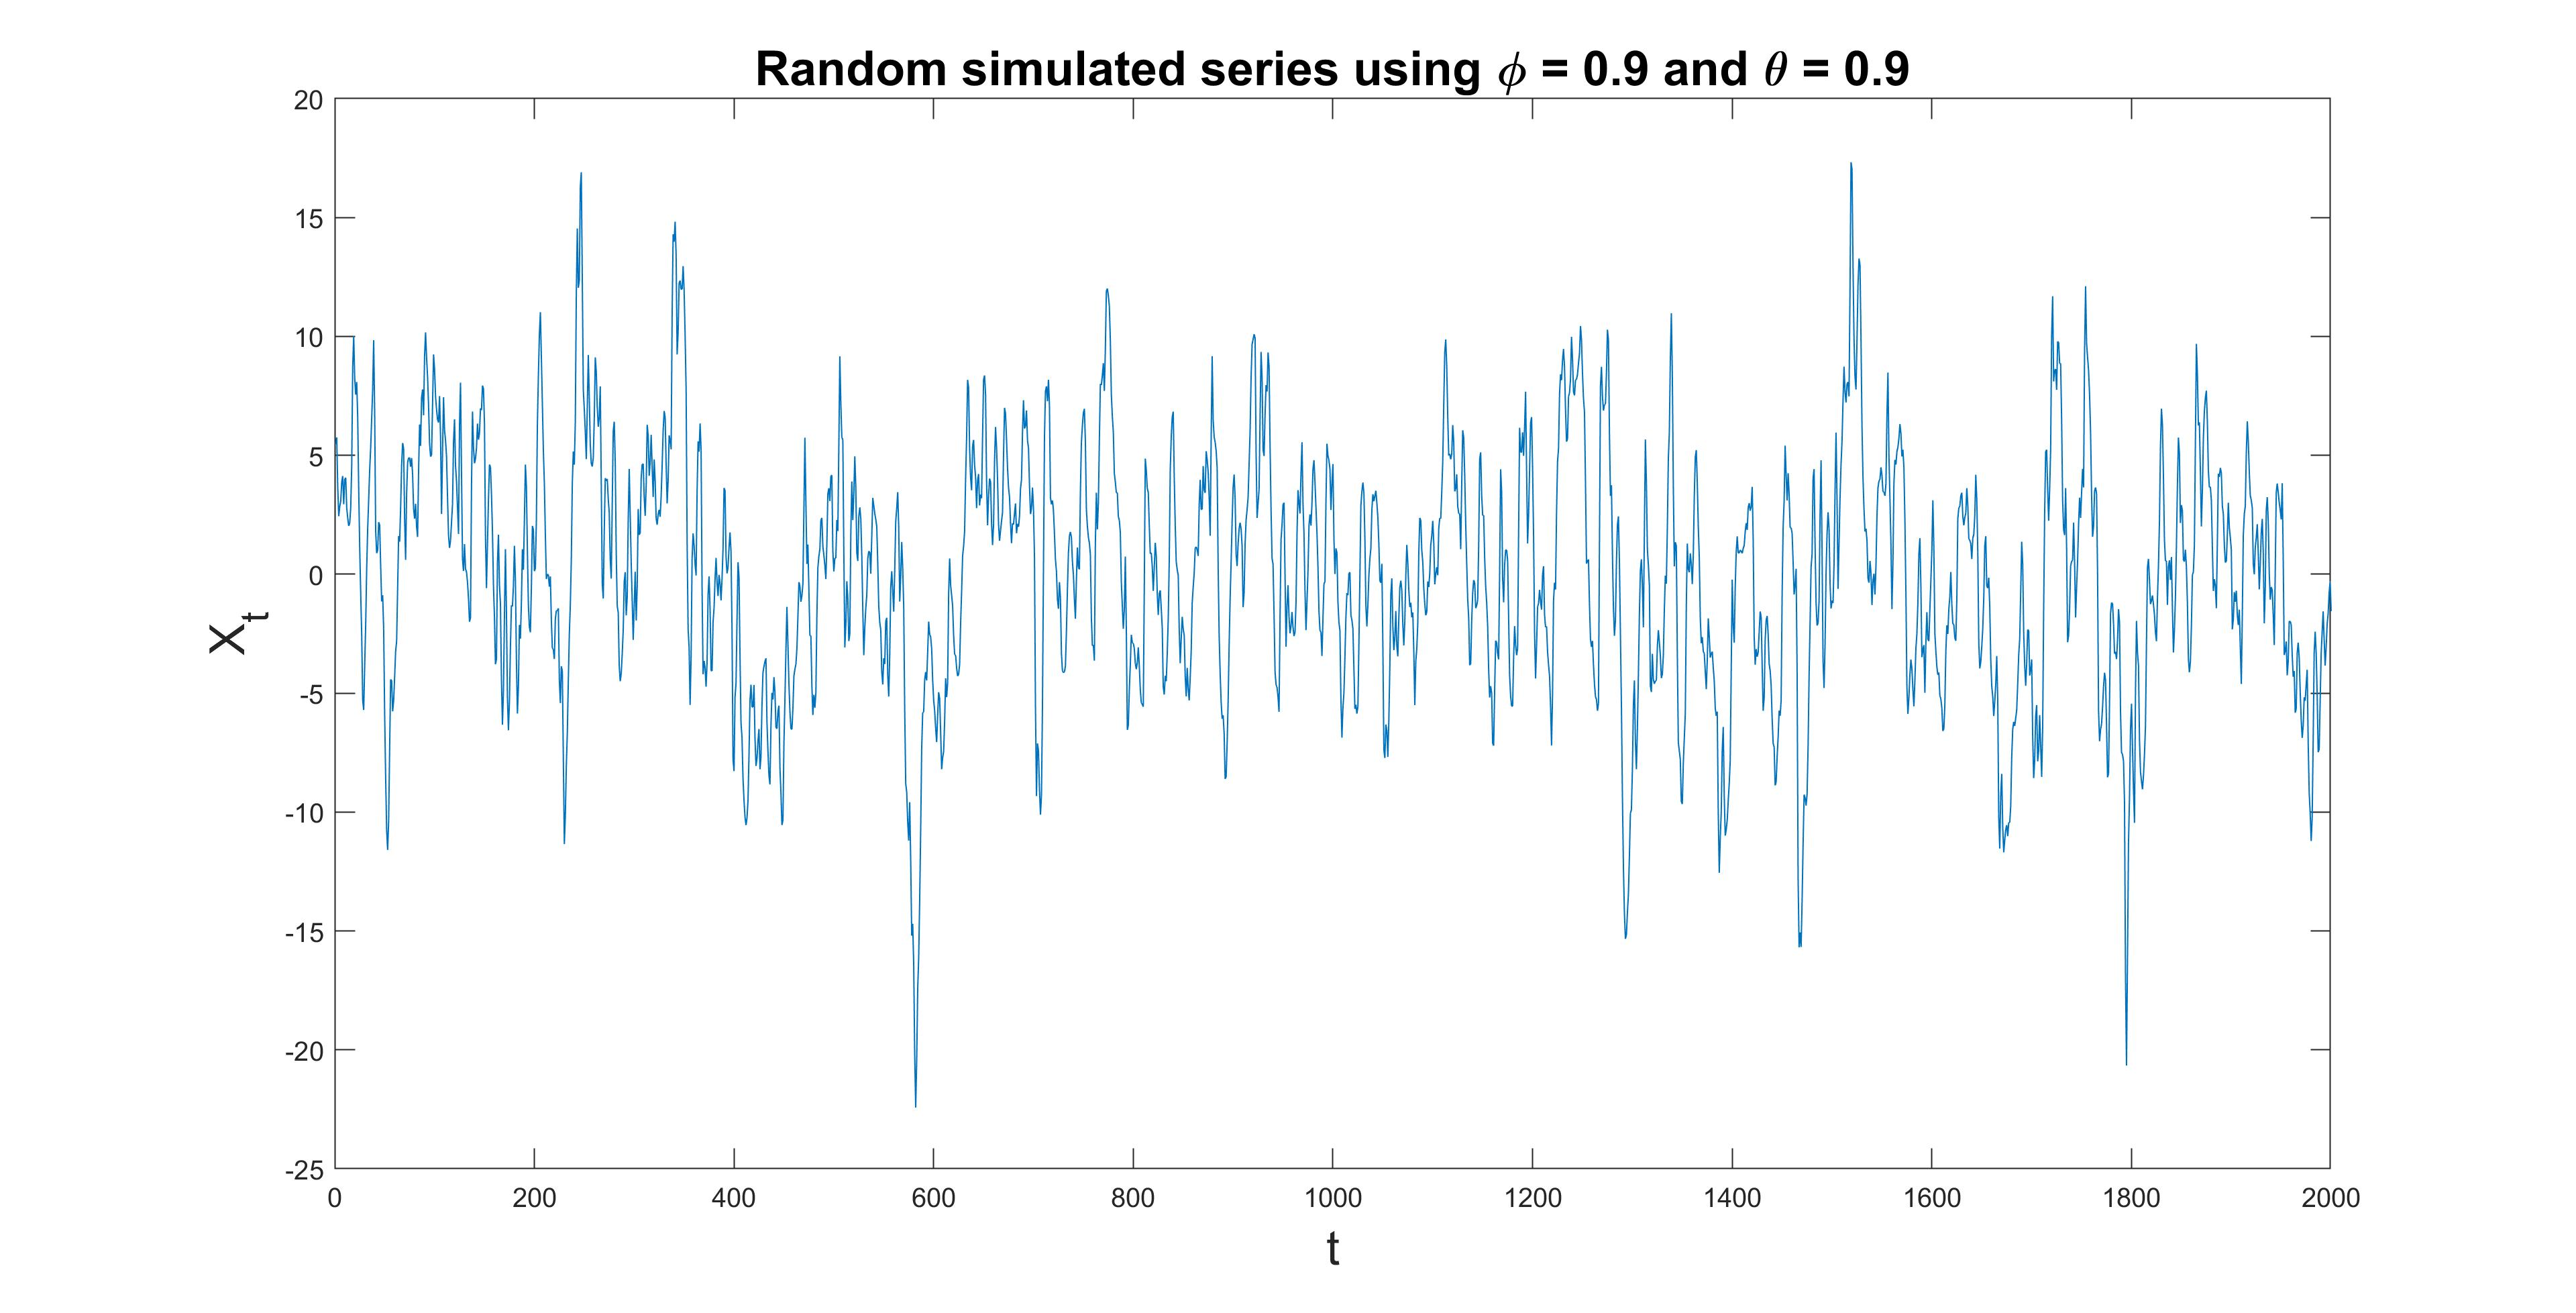
\includegraphics[height=7.25cm, width=1\linewidth]{Figures/results_arma_simdata3.jpg}} 
\end{array}$
\vspace{-0.8cm}
\captionsetup[figure]{font=small,labelfont=small}
\caption{A random simulated series for three levels of serial dependency.}
\label{fig:results_arma_simdata2}
\end{figure}

In total, the grid of different values for $\phi$ and $\theta$ contains $400$ combinations. For each combination, $m=1,000$ time-series are simulated and the VaR is estimated using the POT and BM method. The evaluation metrics RMSE and RMSPE, see equations \eqref{eq:rmse} and \eqref{eq:mape} respectively, are then calculated. These results are displayed in Figure \ref{fig:results_arma_surfaces}. 


\begin{figure}[H]
\begin{tabular}{cc}
(a) RMSE - POT & (b) RMSE - BM (2) \\[6pt]
  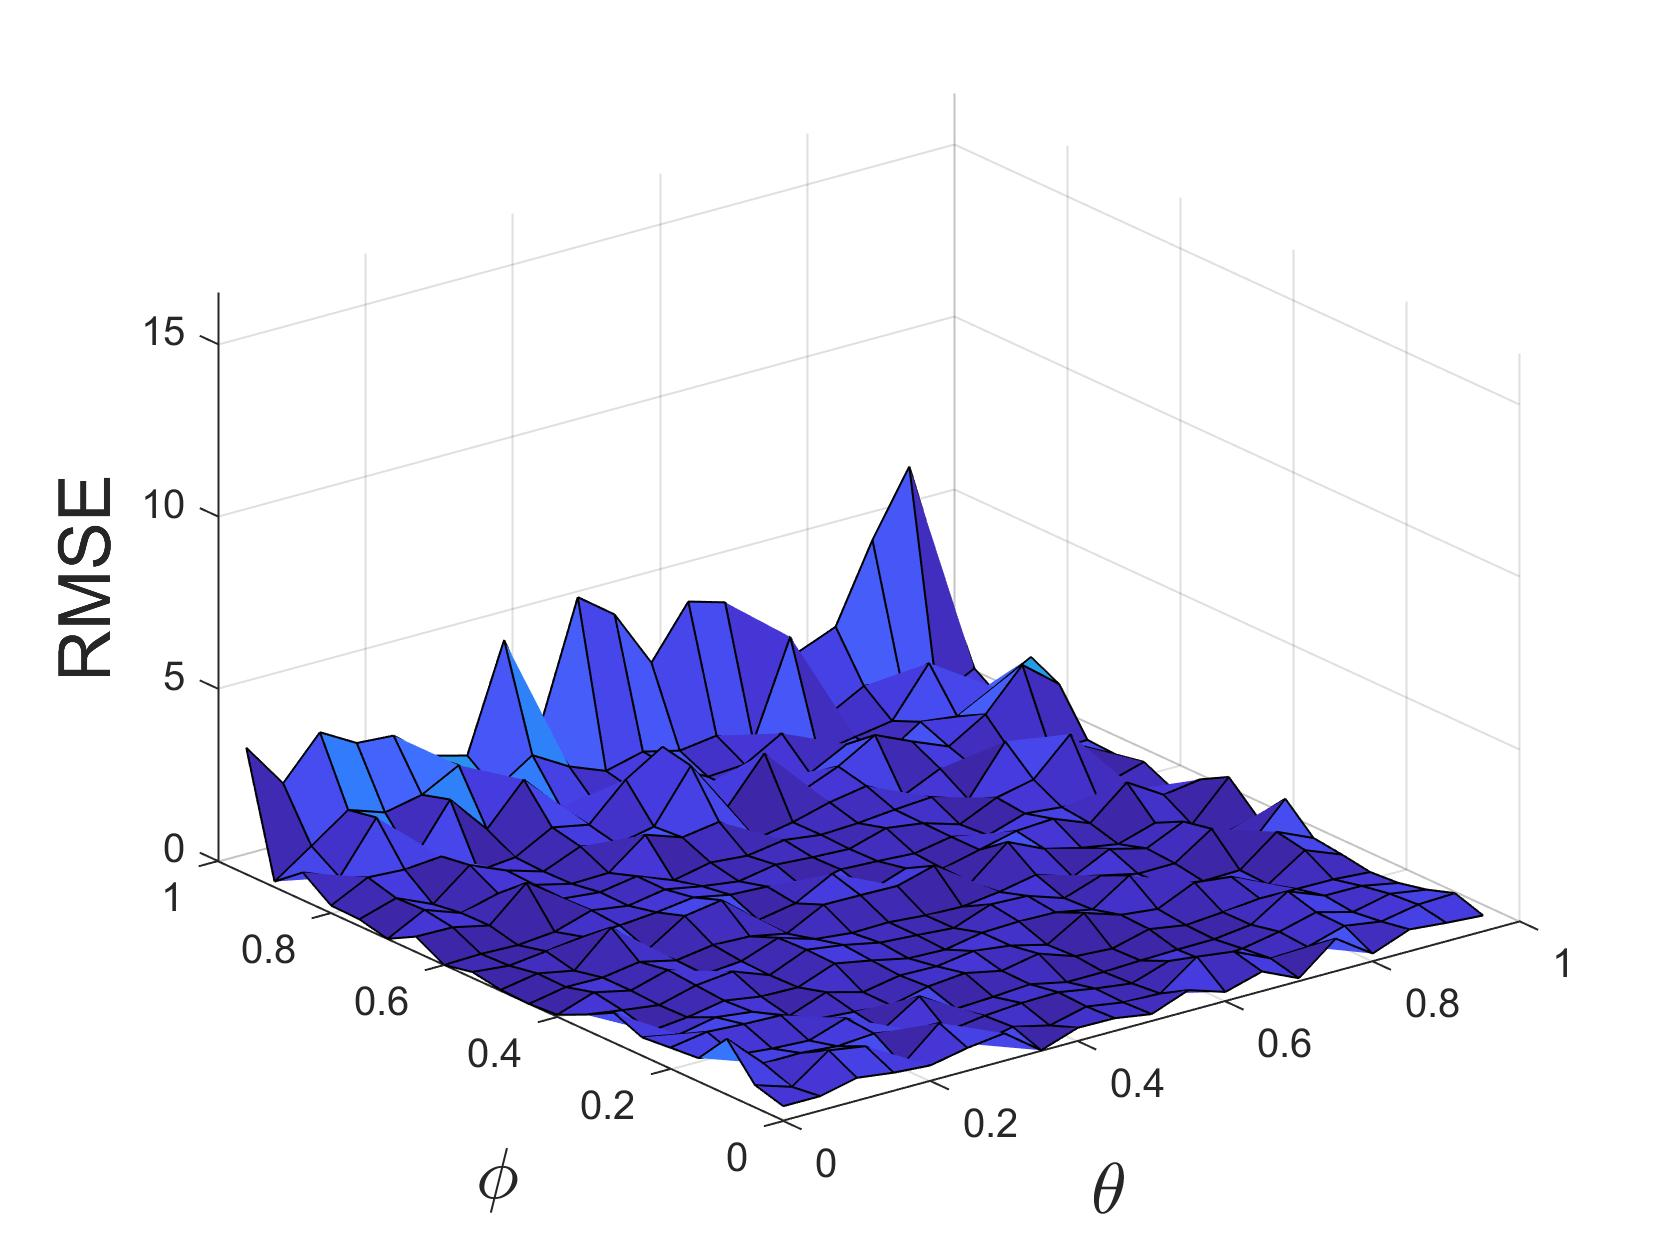
\includegraphics[width=80mm]{Figures/results_rmse_arma_pothill.jpg} &   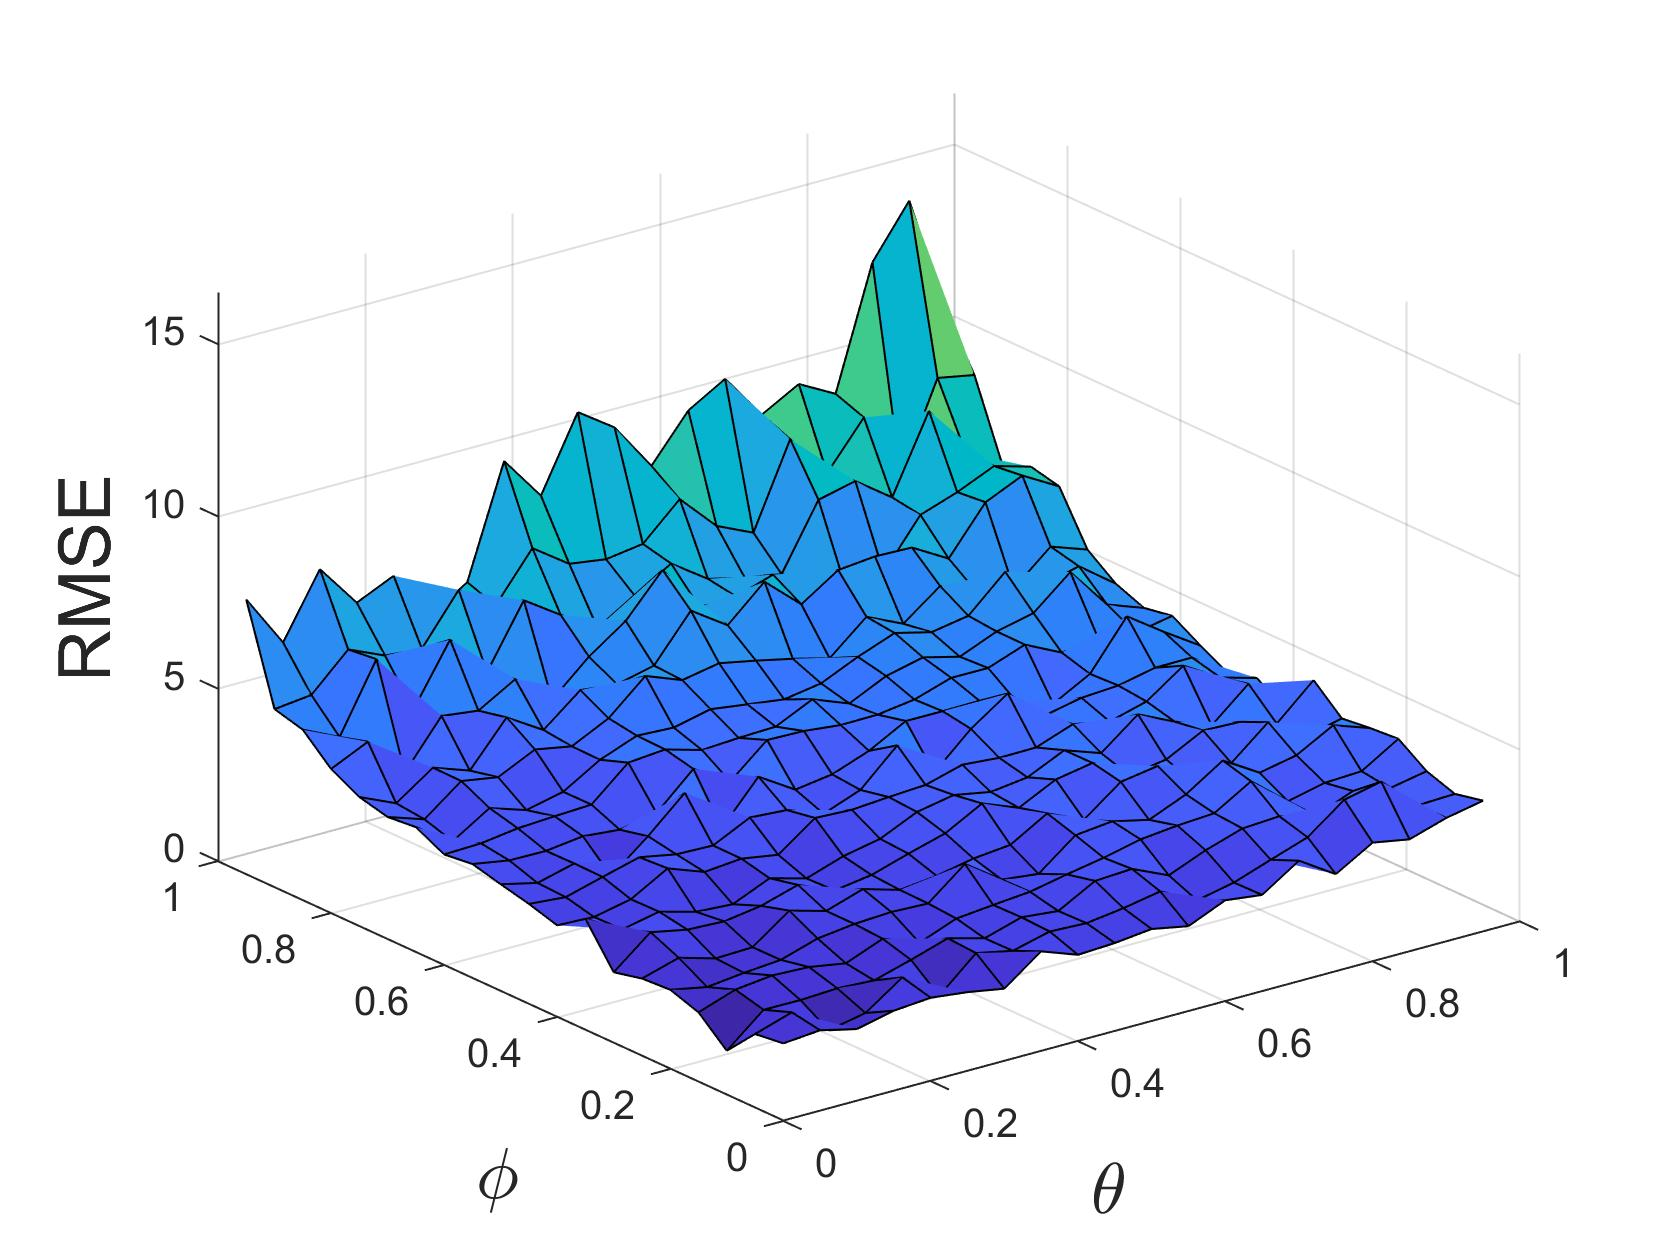
\includegraphics[width=80mm]{Figures/results_rmse_arma_bm2.jpg} \\
  (c) RMSPE - POT & (d) RMSPE - BM (2) \\[6pt]
  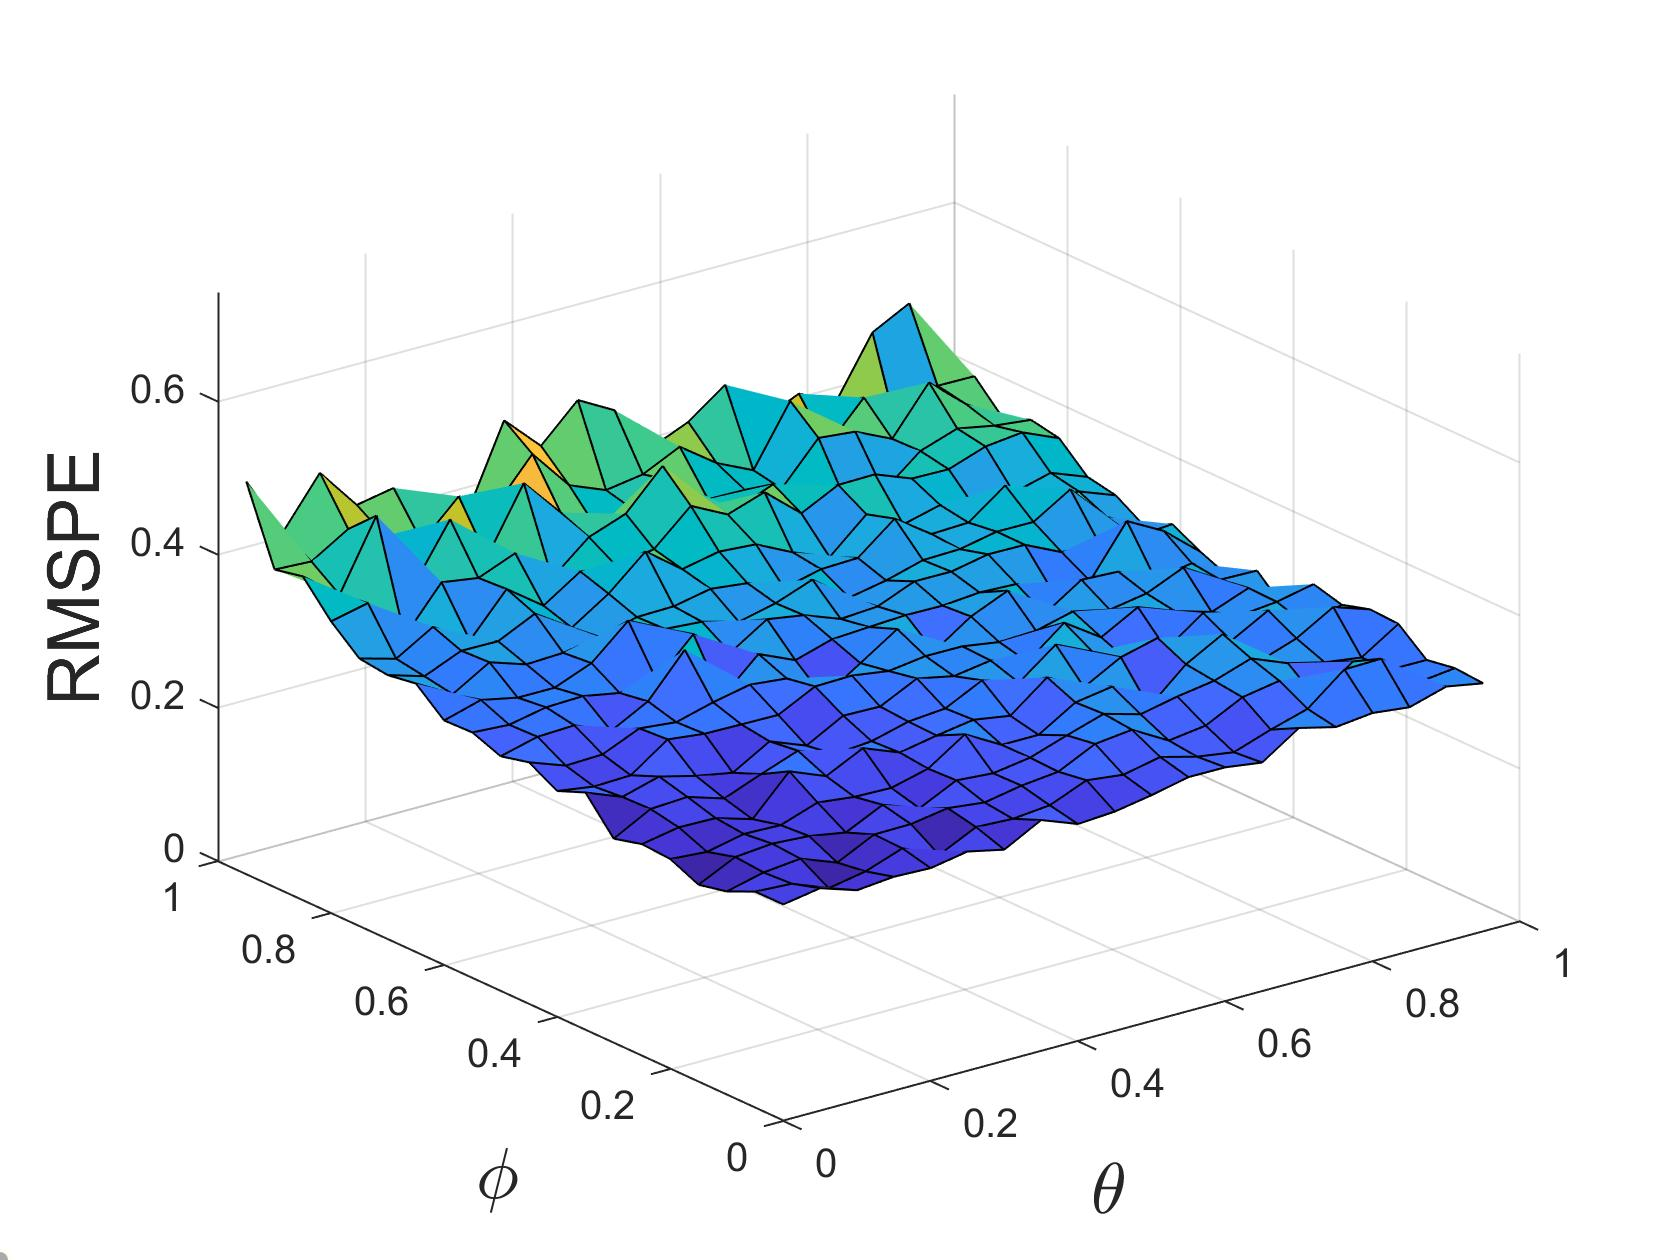
\includegraphics[width=80mm]{Figures/results_mape_arma_pothill.jpg} &   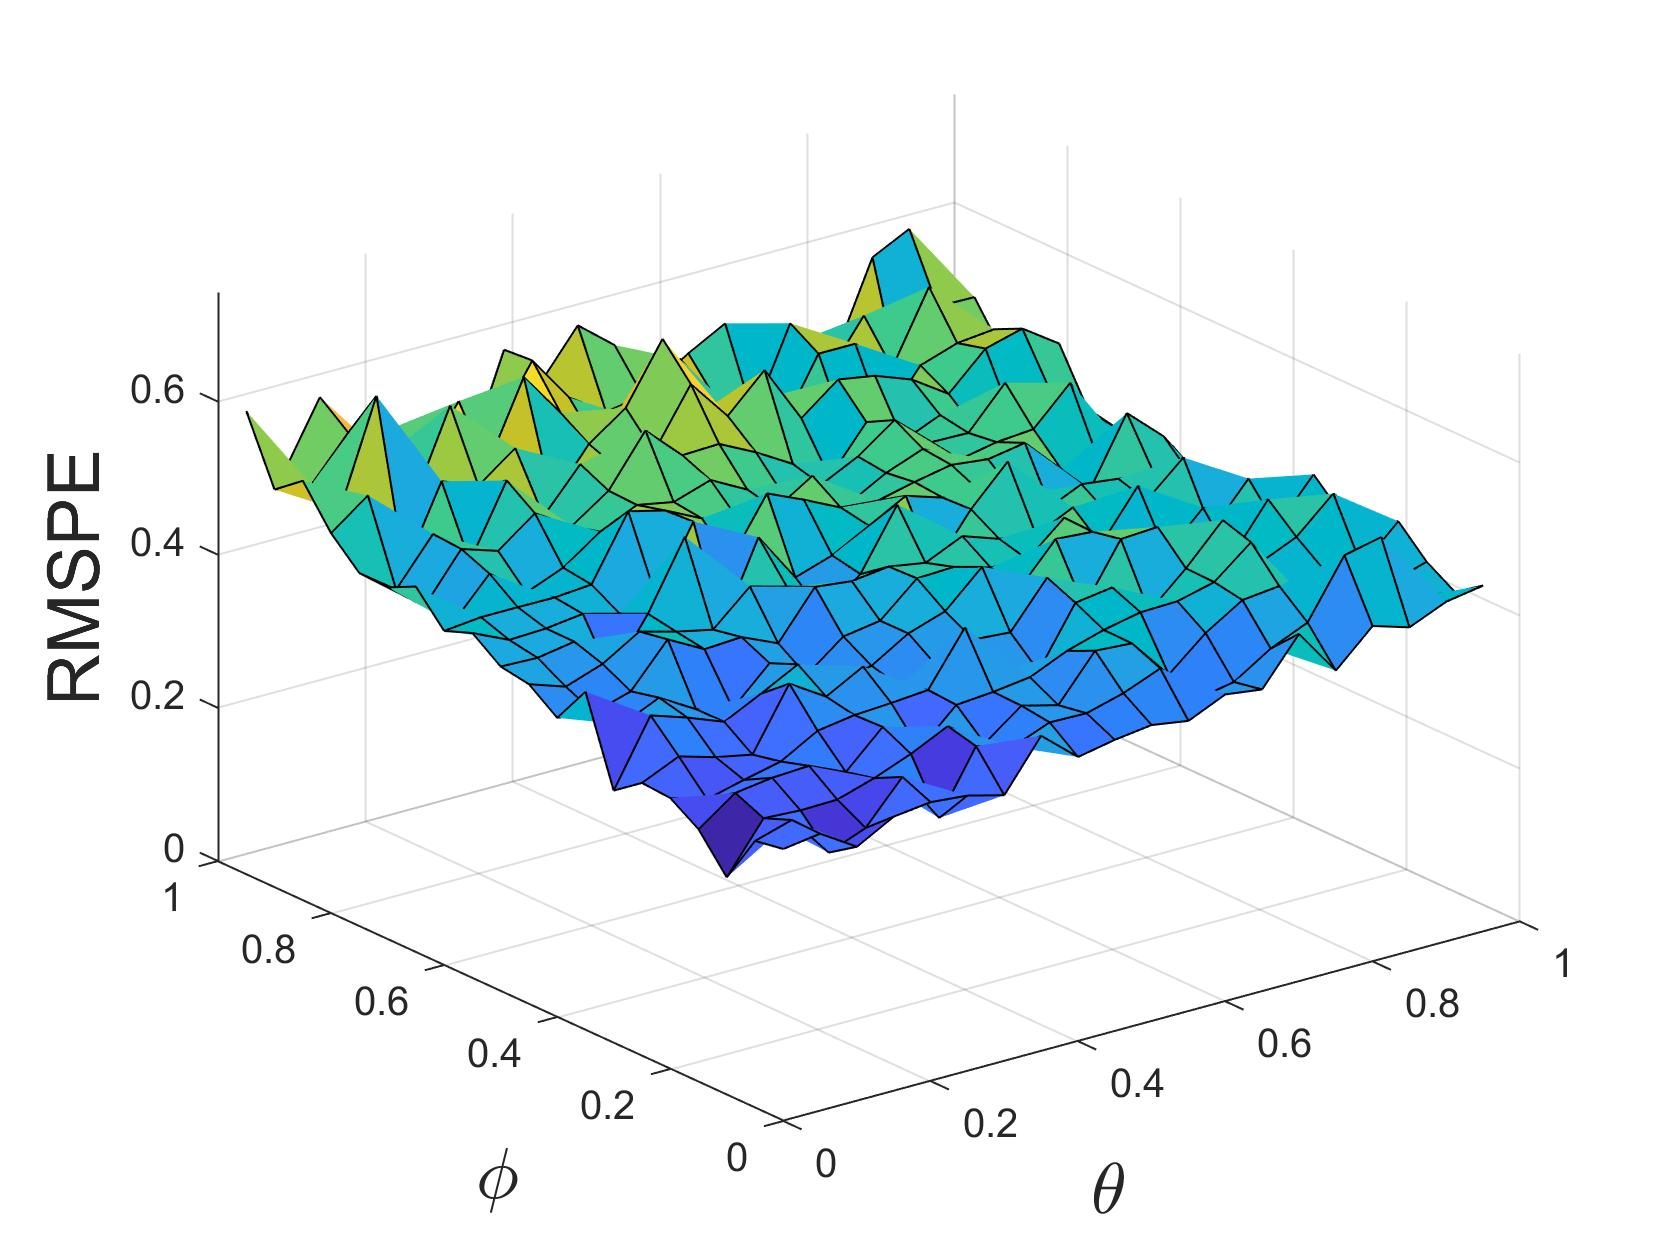
\includegraphics[width=80mm]{Figures/results_mape_arma_bm2.jpg} \\
\end{tabular}
\vspace{-0.8cm}
\captionsetup[figure]{font=small,labelfont=small}
\caption{Surface plots of the evaluation metrics RMSE and RMSPE for increasing $\phi$ and $\theta$. }
\label{fig:results_arma_surfaces}
\end{figure}

Furthermore, for three different values of $\theta$, the comparison of the POT and BM method are displayed in Figure \ref{fig:results_rmse_arma_phi_increase} for the RMSE and Figure \ref{fig:results_mape_arma_phi_increase} for the RMSPE.

\begin{figure}[H]
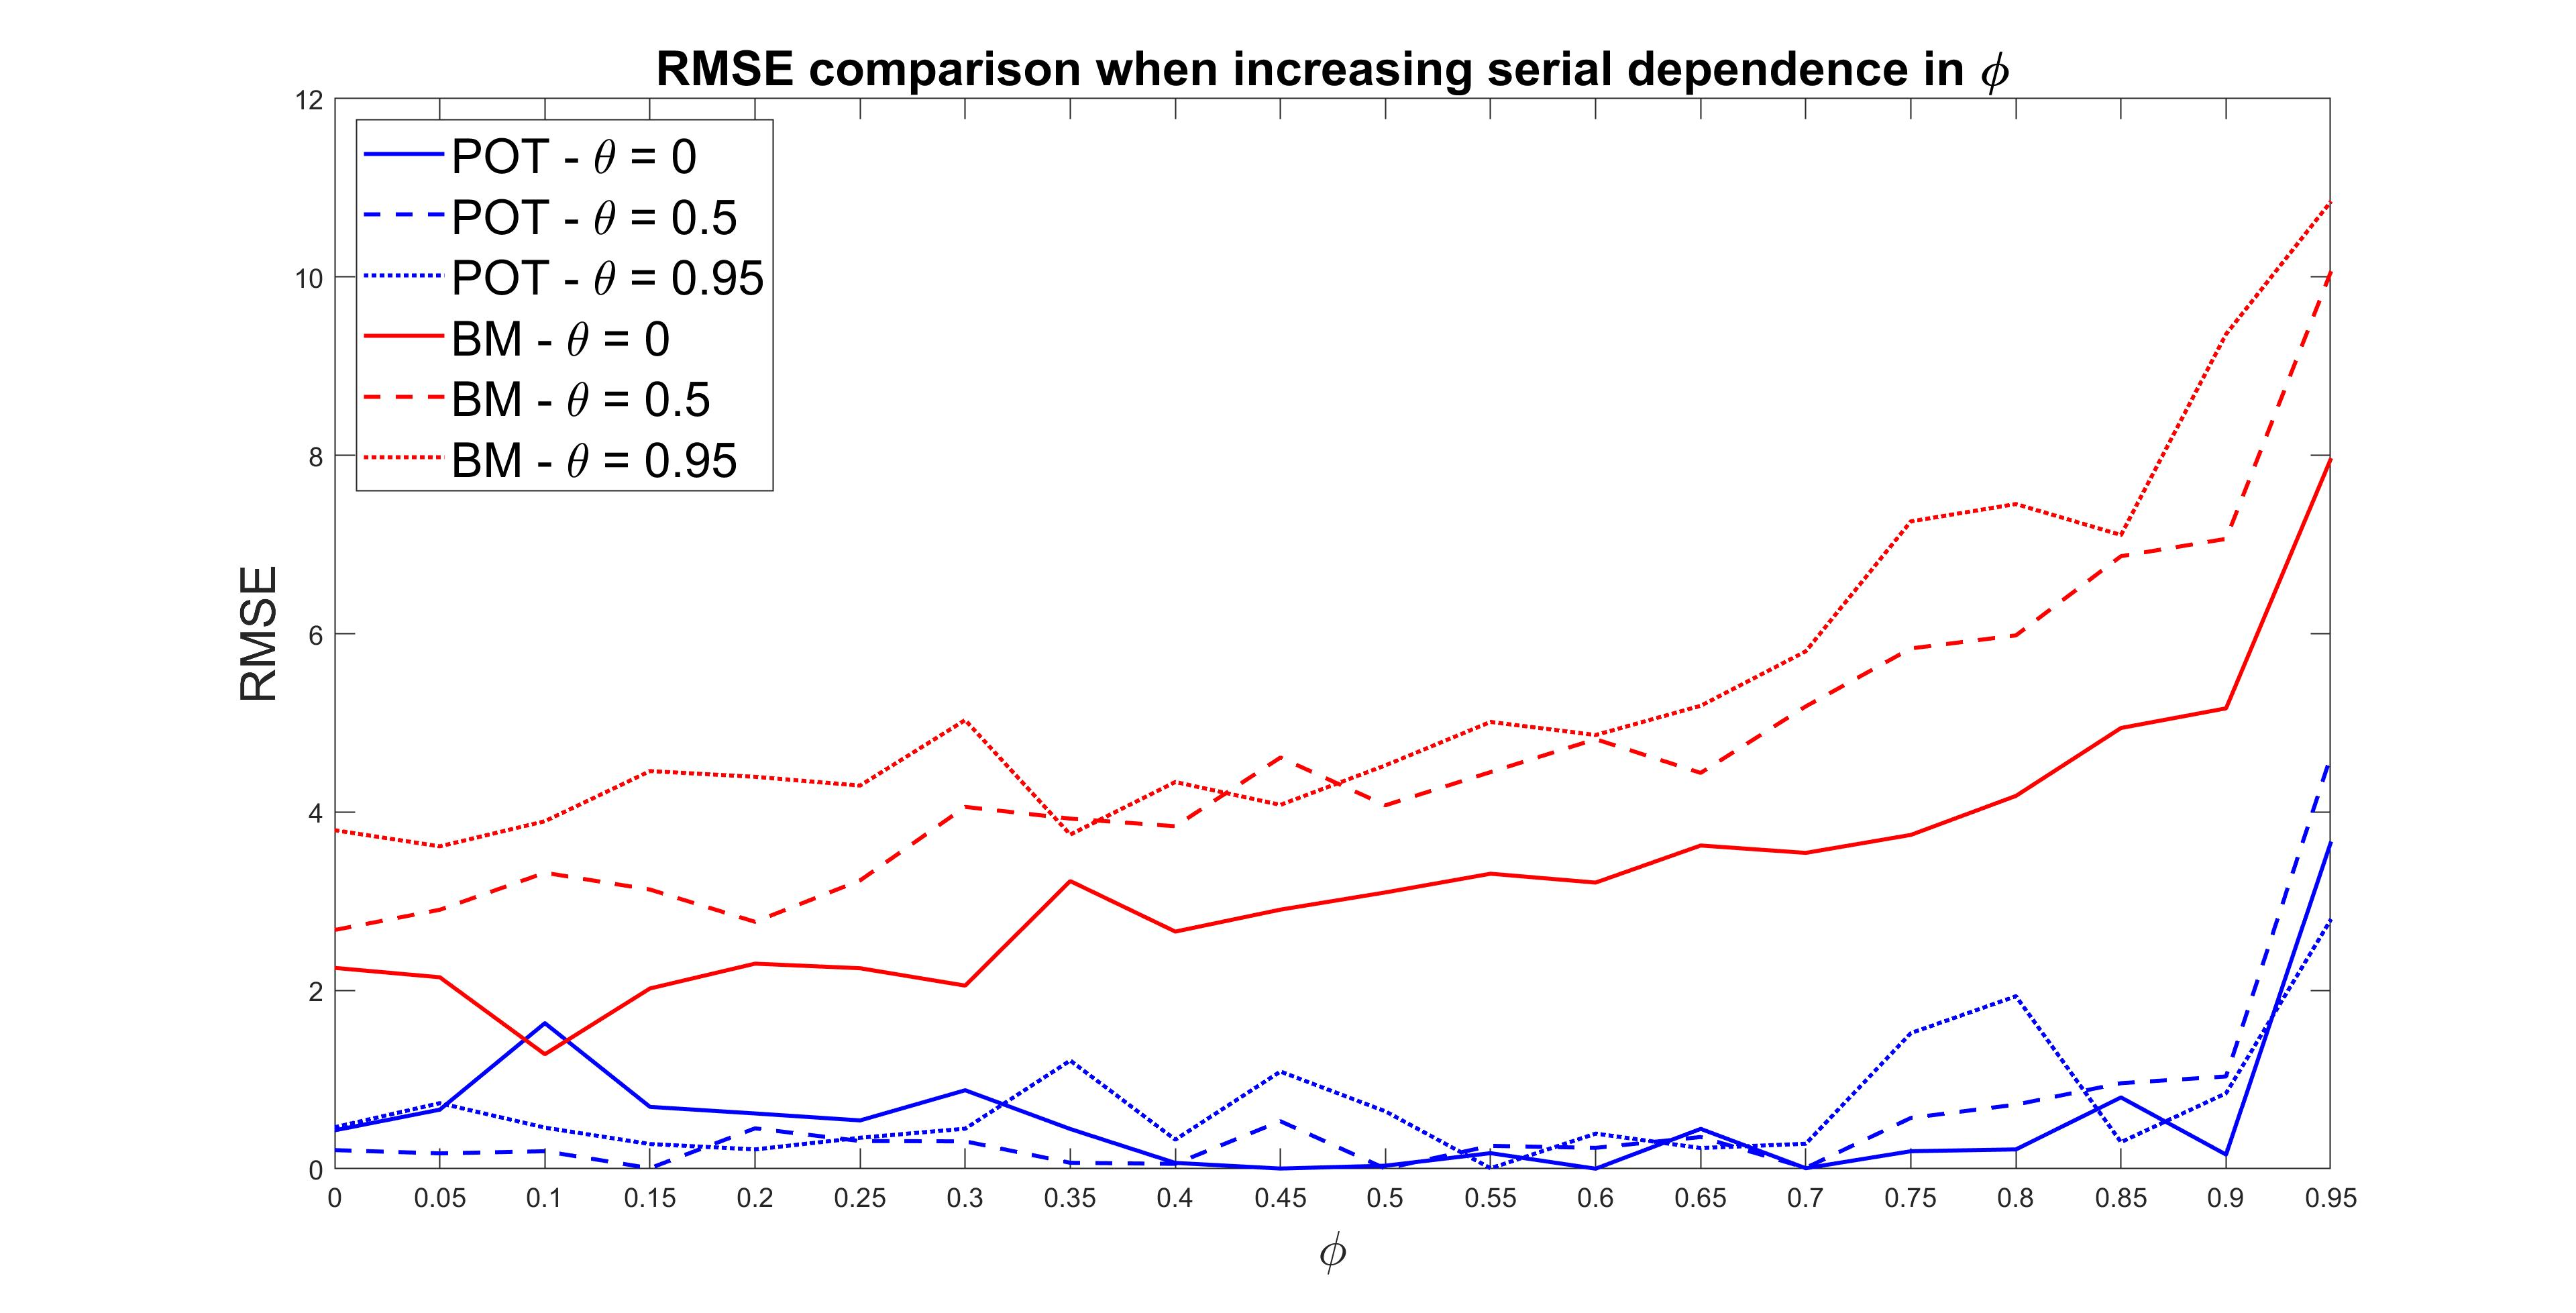
\includegraphics[height=7.8cm, width=\linewidth]{Figures/results_rmse_arma_phi_increase.jpg}
\vspace{-0.8cm}
\captionsetup[figure]{font=small,labelfont=small}
\caption{Comparing the RMSE for increasing $\phi$ at three levels of $\theta$.}
\label{fig:results_rmse_arma_phi_increase}
\end{figure}

\begin{figure}[H]
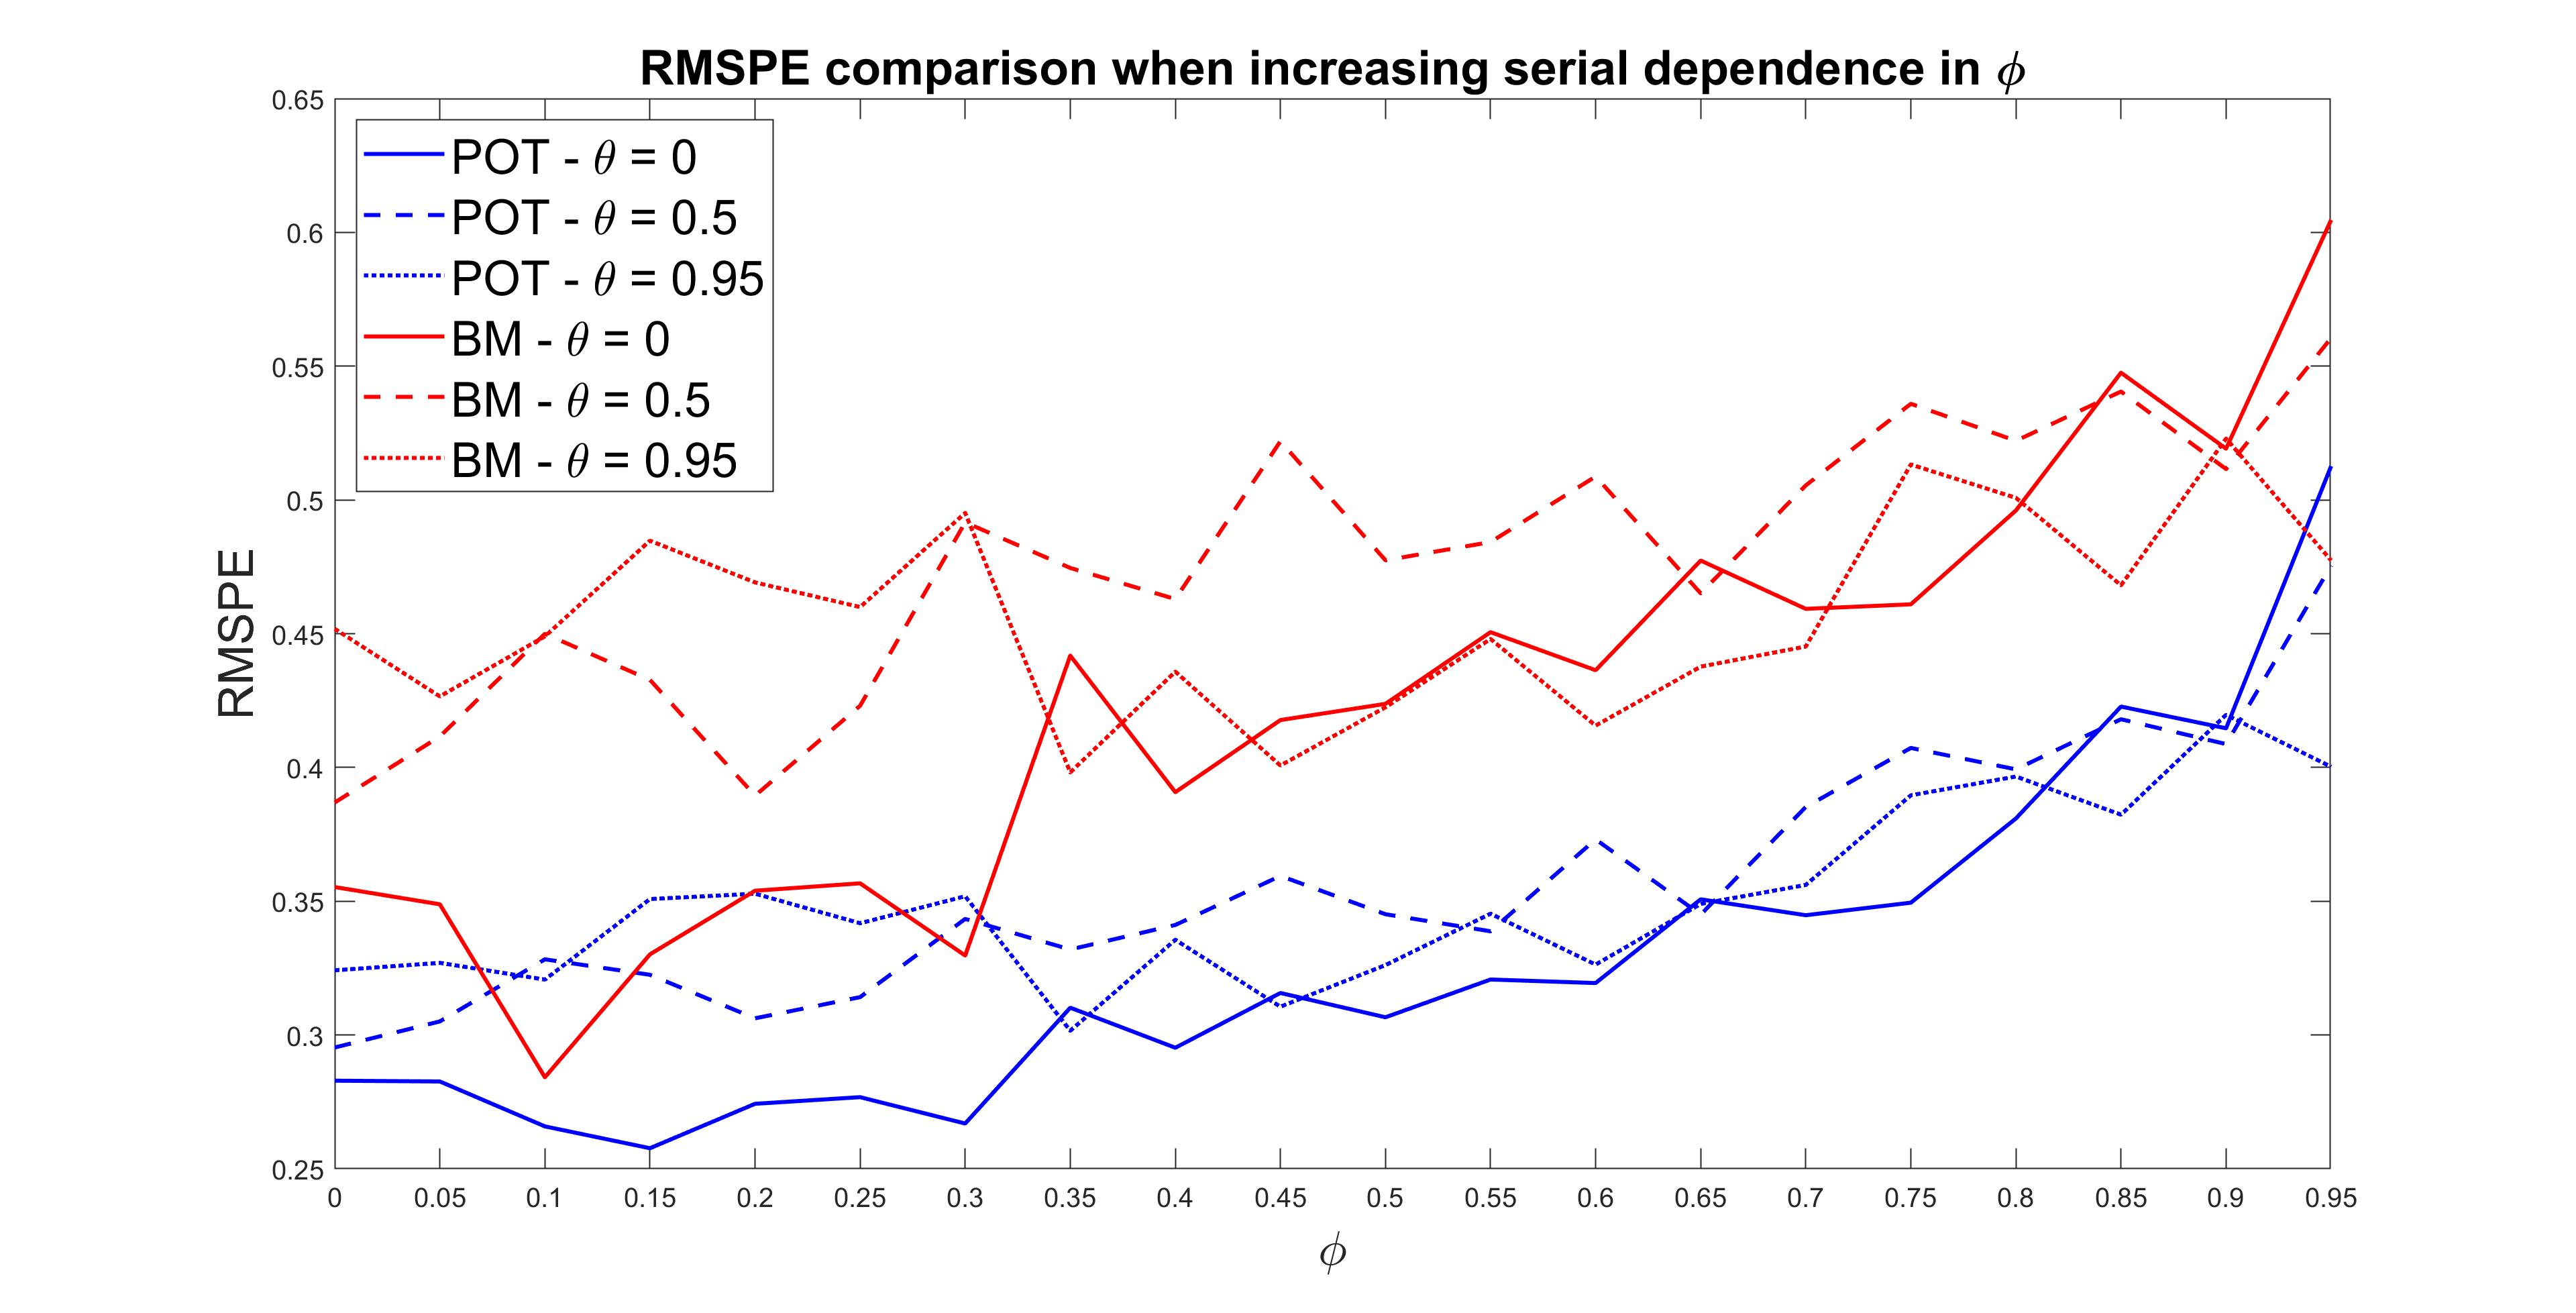
\includegraphics[height=7.8cm, width=\linewidth]{Figures/results_mape_arma_phi_increase.jpg}
\vspace{-0.8cm}
\captionsetup[figure]{font=small,labelfont=small}
\caption{Comparing the RMSPE for increasing $\phi$ at three levels of $\theta$.}
\label{fig:results_mape_arma_phi_increase}
\end{figure}

\newpage



\subsection{Financial Application}



\section{Conclusion}
test
\newpage
\bibliographystyle{apacite}
\bibliography{References}

\newpage
\appendix
\section{Appendix}
\subsection{Maximum Domain of Attraction Examples}
\label{appendixA:maximumdomain}
Recalling the rate of convergence for maxima follows 
\begin{equation}
    \lim_{n\to\infty} P\left(\frac{M_n-b_n}{a_n}\leq x\right)=\lim_{n\to\infty}F^n\left(a_nx+b_n\right)=H\left(x\right),
\end{equation}
two examples are constructed for the underlying distributions: exponential and Pareto. \\

\noindent \textbf{Exponential distribution}\\
Assume the underlying distribution to be exponential with distribution function $F\left(x\right)=1-\exp{\left(-\beta x\right)}$ for $\beta>0$ and $x \geq 0$, then the limiting distribution of maxima can directly be calculated by choosing the normalizing constants $a_n = \frac{1}{\beta}$ and $b_n=\frac{\ln{\left(n\right)}}{\beta}$. It holds that

\begin{equation}
    \begin{split}
    F^n\left(a_nx+b_n\right) &= F^n\left(\frac{x}{\beta}+\frac{\ln{\left(n\right)}}{\beta}\right),\\
    F^n\left(a_nx+b_n\right) &= \left(1-\frac{1}{n}\exp{\left(-x\right)}\right)^n, \quad x\geq-\ln{\left(n\right)}, \\
    \lim_{n\to\infty}F^n\left(a_nx+b_n\right) &= \exp{\left(-\exp{\left(-x\right)}\right)}, \quad x \in \mathbb{R}.
    \end{split}
\end{equation}
Hence, we conclude that $F\in MDA\left(H_0\right)$.\\

\noindent \textbf{Pareto distribution}\\
Assume the underlying distribution to be Pareto with parameters $\alpha$ and $k$ and distribution function $F\left(x\right)=1-\left(\frac{k}{k+x}\right)^\alpha$ for $\alpha>0$, $k>0$ and $x \geq 0$, then the limiting distribution of maxima can directly be calculated by choosing the normalizing constants $a_n = k\frac{n^{\frac{1}{\alpha}}}{\alpha}$ and $b_n=kn^{\frac{1}{\alpha}} - k$. It holds that

\begin{equation}
    \begin{split}
        F^n\left(a_nx+b_n\right) &= F^n\left(k\frac{n^{\frac{1}{\alpha}}}{\alpha}x + \left(kn^{\frac{1}{\alpha}} - k\right)\right),\\
        F^n\left(a_nx+b_n\right) &= \left(1 - \frac{1}{n}\left(1+\frac{x}{\alpha}\right)^{-\alpha}\right)^n, \quad 1+\frac{x}{\alpha}\geq n{-\frac{1}{\alpha}},\\
        \lim_{n\to\infty}F^n\left(a_nx+b_n\right) &= \exp{\left(-\left(1+\frac{x}{\alpha}\right)^{-\alpha}\right)}, \quad 1+\frac{x}{\alpha}>0,
    \end{split}
\end{equation}
Hence, we conclude that $F\in MDA\left(H_{\frac{1}{\alpha}}\right)$.




\subsection{Tables and Graphs}
\renewcommand{\baselinestretch}{0.90}
\newgeometry{left=2.5cm,bottom=2.5cm}
\begin{landscape}
\begin{table}[H]
  \centering
  \caption{Add caption}
  \scalebox{0.9}{
    \begin{tabular}{rl||ccccccccccccccccccc}
          & \multicolumn{1}{r}{} & \multicolumn{19}{c}{\textbf{Theta}} \\
          &       & 0,05  & 0,1   & 0,15  & 0,2   & 0,25  & 0,3   & 0,35  & 0,4   & 0,45  & 0,5   & 0,55  & 0,6   & 0,65  & 0,7   & 0,75  & 0,8   & 0,85  & 0,9   & 0,95 \\ \hline \hline
    \multicolumn{1}{r}{\multirow{19}[1]{*}{\begin{sideways}\textbf{Phi}\end{sideways}}} & 0,05  & 0,25  & 0,22  & 0,26  & 0,21  & 0,24  & 0,25  & 0,26  & 0,24  & 0,28  & 0,27  & 0,25  & 0,26  & 0,34  & 0,29  & 0,29  & 0,29  & 0,28  & 0,33  & 0,31 \\
          & 0,1   & 0,23  & 0,22  & 0,20  & 0,23  & 0,23  & 0,26  & 0,23  & 0,24  & 0,26  & 0,26  & 0,26  & 0,29  & 0,29  & 0,28  & 0,31  & 0,28  & 0,29  & 0,30  & 0,30 \\
          & 0,15  & 0,23  & 0,26  & 0,21  & 0,27  & 0,26  & 0,22  & 0,25  & 0,26  & 0,27  & 0,29  & 0,30  & 0,29  & 0,29  & 0,31  & 0,35  & 0,34  & 0,30  & 0,37  & 0,37 \\
          & 0,2   & 0,20  & 0,24  & 0,24  & 0,25  & 0,28  & 0,26  & 0,26  & 0,28  & 0,27  & 0,29  & 0,29  & 0,27  & 0,29  & 0,30  & 0,34  & 0,34  & 0,34  & 0,37  & 0,36 \\
          & 0,25  & 0,20  & 0,22  & 0,28  & 0,25  & 0,26  & 0,30  & 0,24  & 0,24  & 0,30  & 0,31  & 0,34  & 0,31  & 0,31  & 0,32  & 0,28  & 0,33  & 0,36  & 0,38  & 0,43 \\
          & 0,3   & 0,22  & 0,22  & 0,25  & 0,27  & 0,25  & 0,28  & 0,30  & 0,30  & 0,32  & 0,30  & 0,30  & 0,31  & 0,34  & 0,34  & 0,34  & 0,38  & 0,40  & 0,34  & 0,40 \\
          & 0,35  & 0,22  & 0,27  & 0,27  & 0,26  & 0,26  & 0,28  & 0,31  & 0,30  & 0,27  & 0,38  & 0,32  & 0,32  & 0,31  & 0,40  & 0,39  & 0,46  & 0,40  & 0,34  & 0,40 \\
          & 0,4   & 0,30  & 0,28  & 0,26  & 0,24  & 0,27  & 0,28  & 0,32  & 0,26  & 0,34  & 0,38  & 0,34  & 0,39  & 0,42  & 0,33  & 0,36  & 0,35  & 0,46  & 0,40  & 0,47 \\
          & 0,45  & 0,27  & 0,28  & 0,27  & 0,29  & 0,31  & 0,28  & 0,33  & 0,36  & 0,39  & 0,33  & 0,34  & 0,41  & 0,43  & 0,38  & 0,42  & 0,42  & 0,51  & 0,45  & 0,46 \\
          & 0,5   & 0,27  & 0,31  & 0,27  & 0,32  & 0,34  & 0,34  & 0,33  & 0,35  & 0,42  & 0,43  & 0,45  & 0,38  & 0,44  & 0,42  & 0,47  & 0,42  & 0,46  & 0,45  & 0,45 \\
          & 0,55  & 0,27  & 0,29  & 0,27  & 0,36  & 0,36  & 0,35  & 0,34  & 0,41  & 0,43  & 0,41  & 0,36  & 0,42  & 0,38  & 0,42  & 0,42  & 0,48  & 0,47  & 0,53  & 0,56 \\
          & 0,6   & 0,31  & 0,31  & 0,31  & 0,34  & 0,36  & 0,44  & 0,36  & 0,32  & 0,42  & 0,39  & 0,49  & 0,46  & 0,52  & 0,50  & 0,54  & 0,49  & 0,51  & 0,55  & 0,54 \\
          & 0,65  & 0,36  & 0,33  & 0,43  & 0,36  & 0,44  & 0,43  & 0,40  & 0,40  & 0,46  & 0,45  & 0,53  & 0,54  & 0,50  & 0,56  & 0,57  & 0,53  & 0,65  & 0,57  & 0,66 \\
          & 0,7   & 0,32  & 0,39  & 0,45  & 0,41  & 0,49  & 0,42  & 0,39  & 0,56  & 0,50  & 0,56  & 0,56  & 0,59  & 0,54  & 0,63  & 0,58  & 0,68  & 0,71  & 0,72  & 0,73 \\
          & 0,75  & 0,36  & 0,40  & 0,42  & 0,42  & 0,44  & 0,51  & 0,55  & 0,48  & 0,63  & 0,68  & 0,57  & 0,59  & 0,73  & 0,77  & 0,84  & 0,78  & 0,82  & 0,71  & 0,87 \\
          & 0,8   & 0,50  & 0,58  & 0,54  & 0,50  & 0,65  & 0,55  & 0,64  & 0,61  & 0,81  & 0,76  & 0,71  & 0,93  & 0,80  & 0,67  & 0,79  & 0,93  & 0,84  & 1,01  & 0,91 \\
          & 0,85  & 0,73  & 0,62  & 0,64  & 0,71  & 0,71  & 0,80  & 0,85  & 0,95  & 0,77  & 0,90  & 0,91  & 1,02  & 0,84  & 0,96  & 1,19  & 1,22  & 1,02  & 1,18  & 1,43 \\
          & 0,9   & 0,81  & 1,00  & 0,87  & 1,19  & 0,97  & 1,20  & 1,04  & 1,18  & 1,03  & 1,29  & 1,43  & 1,24  & 1,29  & 1,41  & 1,47  & 1,42  & 1,65  & 1,55  & 1,59 \\
          & 0,95  & 1,88  & 1,72  & 1,88  & 1,89  & 1,70  & 2,00  & 1,93  & 2,14  & 2,19  & 2,51  & 2,49  & 2,02  & 2,57  & 2,32  & 2,78  & 2,66  & 2,91  & 3,17  & 2,94 \\
    \end{tabular}%
    }
  \label{tab:addlabel}%
\end{table}%
\end{landscape}

% Table generated by Excel2LaTeX from sheet 'Sheet1'
\newpage% Table generated by Excel2LaTeX from sheet 'Sheet1'
\renewcommand{\baselinestretch}{0.90}
\newgeometry{left=2.5cm,bottom=2.5cm}
\begin{landscape}
\begin{table}[H]
  \centering
  \caption{Add caption}
  \scalebox{0.9}{
    \begin{tabular}{rl||ccccccccccccccccccc}
          & \multicolumn{1}{r}{} & \multicolumn{19}{c}{\textbf{Theta}} \\
          &       & 0,05  & 0,1   & 0,15  & 0,2   & 0,25  & 0,3   & 0,35  & 0,4   & 0,45  & 0,5   & 0,55  & 0,6   & 0,65  & 0,7   & 0,75  & 0,8   & 0,85  & 0,9   & 0,95 \\ \hline \hline
\multicolumn{1}{r}{\multirow{19}[1]{*}{\begin{sideways}\textbf{Phi}\end{sideways}}} & 0,05  & 0,38  & 0,41  & 0,37  & 0,42  & 0,41  & 0,40  & 0,40  & 0,44  & 0,42  & 0,44  & 0,46  & 0,49  & 0,42  & 0,48  & 0,51  & 0,52  & 0,57  & 0,52  & 0,57 \\
          & 0,1   & 0,40  & 0,41  & 0,44  & 0,42  & 0,43  & 0,40  & 0,45  & 0,46  & 0,45  & 0,46  & 0,48  & 0,47  & 0,49  & 0,50  & 0,51  & 0,56  & 0,57  & 0,57  & 0,59 \\
          & 0,15  & 0,41  & 0,37  & 0,44  & 0,39  & 0,40  & 0,46  & 0,44  & 0,45  & 0,45  & 0,45  & 0,46  & 0,48  & 0,50  & 0,51  & 0,49  & 0,52  & 0,58  & 0,54  & 0,55 \\
          & 0,2   & 0,44  & 0,40  & 0,42  & 0,41  & 0,41  & 0,44  & 0,46  & 0,45  & 0,47  & 0,47  & 0,49  & 0,53  & 0,53  & 0,55  & 0,53  & 0,55  & 0,56  & 0,56  & 0,60 \\
          & 0,25  & 0,46  & 0,44  & 0,39  & 0,43  & 0,44  & 0,41  & 0,49  & 0,50  & 0,48  & 0,47  & 0,46  & 0,51  & 0,53  & 0,56  & 0,61  & 0,58  & 0,57  & 0,58  & 0,56 \\
          & 0,3   & 0,44  & 0,45  & 0,43  & 0,44  & 0,47  & 0,45  & 0,45  & 0,47  & 0,47  & 0,50  & 0,54  & 0,54  & 0,54  & 0,56  & 0,59  & 0,57  & 0,58  & 0,66  & 0,63 \\
          & 0,35  & 0,45  & 0,42  & 0,43  & 0,46  & 0,48  & 0,47  & 0,47  & 0,49  & 0,54  & 0,46  & 0,54  & 0,56  & 0,59  & 0,53  & 0,57  & 0,52  & 0,61  & 0,69  & 0,66 \\
          & 0,4   & 0,39  & 0,43  & 0,46  & 0,50  & 0,49  & 0,51  & 0,48  & 0,57  & 0,51  & 0,49  & 0,55  & 0,53  & 0,53  & 0,63  & 0,64  & 0,66  & 0,58  & 0,67  & 0,64 \\
          & 0,45  & 0,45  & 0,45  & 0,48  & 0,48  & 0,48  & 0,54  & 0,51  & 0,50  & 0,49  & 0,57  & 0,59  & 0,56  & 0,57  & 0,62  & 0,61  & 0,65  & 0,59  & 0,67  & 0,69 \\
          & 0,5   & 0,47  & 0,44  & 0,50  & 0,47  & 0,48  & 0,50  & 0,54  & 0,54  & 0,51  & 0,52  & 0,53  & 0,63  & 0,59  & 0,65  & 0,63  & 0,71  & 0,70  & 0,72  & 0,76 \\
          & 0,55  & 0,50  & 0,49  & 0,54  & 0,47  & 0,50  & 0,54  & 0,57  & 0,53  & 0,54  & 0,59  & 0,67  & 0,63  & 0,70  & 0,69  & 0,73  & 0,71  & 0,74  & 0,73  & 0,72 \\
          & 0,6   & 0,49  & 0,51  & 0,53  & 0,54  & 0,56  & 0,49  & 0,60  & 0,67  & 0,59  & 0,66  & 0,60  & 0,66  & 0,64  & 0,69  & 0,69  & 0,77  & 0,77  & 0,79  & 0,83 \\
          & 0,65  & 0,48  & 0,54  & 0,48  & 0,56  & 0,52  & 0,57  & 0,62  & 0,66  & 0,63  & 0,69  & 0,64  & 0,66  & 0,72  & 0,71  & 0,74  & 0,80  & 0,73  & 0,84  & 0,77 \\
          & 0,7   & 0,57  & 0,54  & 0,51  & 0,58  & 0,54  & 0,64  & 0,70  & 0,59  & 0,67  & 0,65  & 0,70  & 0,70  & 0,78  & 0,74  & 0,84  & 0,76  & 0,78  & 0,81  & 0,83 \\
          & 0,75  & 0,60  & 0,61  & 0,63  & 0,66  & 0,68  & 0,66  & 0,67  & 0,76  & 0,67  & 0,64  & 0,80  & 0,82  & 0,71  & 0,72  & 0,70  & 0,80  & 0,81  & 0,96  & 0,84 \\
          & 0,8   & 0,57  & 0,52  & 0,61  & 0,68  & 0,59  & 0,74  & 0,69  & 0,76  & 0,61  & 0,72  & 0,82  & 0,63  & 0,82  & 1,01  & 0,93  & 0,82  & 0,95  & 0,84  & 0,99 \\
          & 0,85  & 0,47  & 0,64  & 0,65  & 0,65  & 0,71  & 0,67  & 0,67  & 0,63  & 0,86  & 0,78  & 0,81  & 0,76  & 0,99  & 0,94  & 0,76  & 0,82  & 1,04  & 0,93  & 0,75 \\
          & 0,9   & 0,61  & 0,47  & 0,67  & 0,41  & 0,69  & 0,53  & 0,76  & 0,66  & 0,89  & 0,70  & 0,59  & 0,86  & 0,89  & 0,82  & 0,83  & 0,93  & 0,76  & 0,95  & 0,99 \\
          & 0,95  & 0,17  & 0,02  & 0,02  & 0,01  & 0,27  & 0,07  & 0,22  & 0,05  & 0,08  & 0,12  & 0,00  & 0,44  & 0,01  & 0,37  & 0,01  & 0,21  & 0,06  & 0,24  & 0,11 \\
    \end{tabular}%
  \label{tab:addlabel}%
  }
\end{table}%
\end{landscape}

% Table generated by Excel2LaTeX from sheet 'Sheet1'
\newpage% Table generated by Excel2LaTeX from sheet 'Sheet1'
\renewcommand{\baselinestretch}{0.90}
\newgeometry{left=2.5cm,bottom=2.5cm}
\begin{landscape}
\begin{table}[H]
  \centering
  \caption{Add caption}
  \scalebox{0.9}{
    \begin{tabular}{rl||ccccccccccccccccccc}
          & \multicolumn{1}{r}{} & \multicolumn{19}{c}{\textbf{Theta}} \\
          &       & 0,05  & 0,1   & 0,15  & 0,2   & 0,25  & 0,3   & 0,35  & 0,4   & 0,45  & 0,5   & 0,55  & 0,6   & 0,65  & 0,7   & 0,75  & 0,8   & 0,85  & 0,9   & 0,95 \\ \hline \hline
    \multicolumn{1}{r}{\multirow{19}[1]{*}{\begin{sideways}\textbf{Phi}\end{sideways}}} & 0,05  & 0,22  & 0,19  & 0,23  & 0,18  & 0,21  & 0,22  & 0,23  & 0,20  & 0,23  & 0,23  & 0,20  & 0,21  & 0,28  & 0,23  & 0,23  & 0,23  & 0,22  & 0,26  & 0,24 \\
          & 0,1   & 0,20  & 0,19  & 0,17  & 0,20  & 0,20  & 0,22  & 0,19  & 0,19  & 0,22  & 0,21  & 0,21  & 0,23  & 0,23  & 0,22  & 0,24  & 0,21  & 0,23  & 0,23  & 0,23 \\
          & 0,15  & 0,20  & 0,23  & 0,17  & 0,23  & 0,22  & 0,18  & 0,21  & 0,22  & 0,22  & 0,23  & 0,24  & 0,23  & 0,23  & 0,25  & 0,29  & 0,27  & 0,23  & 0,29  & 0,30 \\
          & 0,2   & 0,17  & 0,21  & 0,20  & 0,22  & 0,24  & 0,21  & 0,21  & 0,23  & 0,22  & 0,23  & 0,23  & 0,21  & 0,23  & 0,23  & 0,27  & 0,27  & 0,27  & 0,30  & 0,28 \\
          & 0,25  & 0,16  & 0,18  & 0,24  & 0,21  & 0,21  & 0,25  & 0,19  & 0,19  & 0,24  & 0,25  & 0,27  & 0,24  & 0,24  & 0,24  & 0,21  & 0,26  & 0,28  & 0,30  & 0,34 \\
          & 0,3   & 0,18  & 0,18  & 0,21  & 0,22  & 0,20  & 0,23  & 0,25  & 0,24  & 0,26  & 0,24  & 0,23  & 0,24  & 0,26  & 0,26  & 0,26  & 0,29  & 0,32  & 0,25  & 0,31 \\
          & 0,35  & 0,19  & 0,23  & 0,23  & 0,21  & 0,21  & 0,22  & 0,25  & 0,24  & 0,21  & 0,32  & 0,25  & 0,24  & 0,23  & 0,32  & 0,30  & 0,38  & 0,31  & 0,25  & 0,31 \\
          & 0,4   & 0,26  & 0,23  & 0,21  & 0,18  & 0,21  & 0,21  & 0,25  & 0,19  & 0,27  & 0,30  & 0,27  & 0,30  & 0,34  & 0,24  & 0,27  & 0,26  & 0,36  & 0,30  & 0,37 \\
          & 0,45  & 0,22  & 0,22  & 0,22  & 0,23  & 0,25  & 0,21  & 0,25  & 0,29  & 0,31  & 0,25  & 0,26  & 0,32  & 0,33  & 0,29  & 0,33  & 0,32  & 0,40  & 0,35  & 0,35 \\
          & 0,5   & 0,21  & 0,25  & 0,21  & 0,25  & 0,27  & 0,27  & 0,26  & 0,27  & 0,33  & 0,34  & 0,36  & 0,29  & 0,35  & 0,32  & 0,36  & 0,31  & 0,36  & 0,34  & 0,33 \\
          & 0,55  & 0,20  & 0,22  & 0,21  & 0,28  & 0,28  & 0,27  & 0,25  & 0,32  & 0,34  & 0,31  & 0,26  & 0,32  & 0,27  & 0,32  & 0,30  & 0,36  & 0,36  & 0,41  & 0,44 \\
          & 0,6   & 0,24  & 0,24  & 0,24  & 0,26  & 0,27  & 0,35  & 0,26  & 0,22  & 0,32  & 0,29  & 0,39  & 0,34  & 0,41  & 0,39  & 0,42  & 0,37  & 0,39  & 0,42  & 0,41 \\
          & 0,65  & 0,28  & 0,25  & 0,34  & 0,26  & 0,34  & 0,34  & 0,30  & 0,29  & 0,36  & 0,34  & 0,41  & 0,42  & 0,38  & 0,44  & 0,43  & 0,40  & 0,52  & 0,43  & 0,52 \\
          & 0,7   & 0,23  & 0,29  & 0,36  & 0,31  & 0,38  & 0,31  & 0,29  & 0,45  & 0,38  & 0,44  & 0,44  & 0,47  & 0,41  & 0,50  & 0,44  & 0,54  & 0,56  & 0,57  & 0,59 \\
          & 0,75  & 0,26  & 0,29  & 0,31  & 0,31  & 0,32  & 0,39  & 0,43  & 0,35  & 0,51  & 0,56  & 0,43  & 0,46  & 0,60  & 0,63  & 0,70  & 0,63  & 0,67  & 0,57  & 0,72 \\
          & 0,8   & 0,38  & 0,46  & 0,42  & 0,37  & 0,53  & 0,43  & 0,51  & 0,48  & 0,67  & 0,62  & 0,57  & 0,80  & 0,66  & 0,53  & 0,63  & 0,78  & 0,68  & 0,86  & 0,74 \\
          & 0,85  & 0,59  & 0,48  & 0,50  & 0,57  & 0,58  & 0,66  & 0,70  & 0,81  & 0,63  & 0,76  & 0,77  & 0,88  & 0,69  & 0,81  & 1,02  & 1,05  & 0,84  & 1,01  & 1,26 \\
          & 0,9   & 0,65  & 0,84  & 0,72  & 1,04  & 0,81  & 1,04  & 0,88  & 1,03  & 0,88  & 1,13  & 1,28  & 1,06  & 1,12  & 1,25  & 1,30  & 1,23  & 1,48  & 1,40  & 1,41 \\
          & 0,95  & 1,65  & 1,52  & 1,68  & 1,68  & 1,49  & 1,81  & 1,70  & 1,93  & 2,00  & 2,29  & 2,25  & 1,80  & 2,40  & 2,11  & 2,56  & 2,42  & 2,66  & 2,95  & 2,71 \\
    \end{tabular}%
  \label{tab:addlabel}%
  }
\end{table}%
\end{landscape}


% Table generated by Excel2LaTeX from sheet 'Sheet1'
\newpage% Table generated by Excel2LaTeX from sheet 'Sheet1'
\renewcommand{\baselinestretch}{0.90}
\newgeometry{left=2.5cm,bottom=2.5cm}
\begin{landscape}
\begin{table}[H]
  \centering
  \caption{Add caption}
  \scalebox{0.9}{
    \begin{tabular}{rl||ccccccccccccccccccc}
          & \multicolumn{1}{r}{} & \multicolumn{19}{c}{\textbf{Theta}} \\
          &       & 0,05  & 0,1   & 0,15  & 0,2   & 0,25  & 0,3   & 0,35  & 0,4   & 0,45  & 0,5   & 0,55  & 0,6   & 0,65  & 0,7   & 0,75  & 0,8   & 0,85  & 0,9   & 0,95 \\ \hline \hline
    \multicolumn{1}{r}{\multirow{19}[1]{*}{\begin{sideways}\textbf{Phi}\end{sideways}}} & 0,05  & 0,20  & 0,17  & 0,21  & 0,16  & 0,19  & 0,20  & 0,21  & 0,18  & 0,21  & 0,20  & 0,18  & 0,18  & 0,26  & 0,21  & 0,20  & 0,20  & 0,19  & 0,24  & 0,21 \\
          & 0,1   & 0,18  & 0,18  & 0,15  & 0,18  & 0,18  & 0,20  & 0,17  & 0,17  & 0,19  & 0,19  & 0,18  & 0,21  & 0,20  & 0,20  & 0,21  & 0,18  & 0,20  & 0,20  & 0,20 \\
          & 0,15  & 0,18  & 0,22  & 0,15  & 0,21  & 0,20  & 0,16  & 0,19  & 0,19  & 0,19  & 0,21  & 0,21  & 0,20  & 0,20  & 0,22  & 0,26  & 0,24  & 0,20  & 0,26  & 0,26 \\
          & 0,2   & 0,15  & 0,19  & 0,18  & 0,20  & 0,21  & 0,19  & 0,19  & 0,20  & 0,19  & 0,21  & 0,20  & 0,18  & 0,20  & 0,20  & 0,24  & 0,23  & 0,24  & 0,26  & 0,25 \\
          & 0,25  & 0,14  & 0,16  & 0,22  & 0,19  & 0,19  & 0,23  & 0,16  & 0,16  & 0,21  & 0,22  & 0,25  & 0,21  & 0,21  & 0,21  & 0,17  & 0,22  & 0,24  & 0,26  & 0,30 \\
          & 0,3   & 0,16  & 0,16  & 0,19  & 0,20  & 0,18  & 0,20  & 0,22  & 0,21  & 0,23  & 0,21  & 0,19  & 0,20  & 0,23  & 0,23  & 0,22  & 0,25  & 0,28  & 0,21  & 0,27 \\
          & 0,35  & 0,16  & 0,21  & 0,20  & 0,19  & 0,18  & 0,19  & 0,22  & 0,21  & 0,17  & 0,28  & 0,21  & 0,21  & 0,20  & 0,28  & 0,26  & 0,34  & 0,27  & 0,21  & 0,26 \\
          & 0,4   & 0,23  & 0,21  & 0,18  & 0,16  & 0,18  & 0,18  & 0,22  & 0,15  & 0,24  & 0,27  & 0,23  & 0,27  & 0,30  & 0,20  & 0,23  & 0,22  & 0,32  & 0,26  & 0,33 \\
          & 0,45  & 0,20  & 0,20  & 0,19  & 0,20  & 0,22  & 0,18  & 0,22  & 0,26  & 0,28  & 0,22  & 0,22  & 0,28  & 0,29  & 0,24  & 0,28  & 0,27  & 0,35  & 0,30  & 0,30 \\
          & 0,5   & 0,19  & 0,22  & 0,18  & 0,22  & 0,24  & 0,23  & 0,22  & 0,23  & 0,29  & 0,30  & 0,31  & 0,24  & 0,30  & 0,27  & 0,31  & 0,26  & 0,31  & 0,29  & 0,28 \\
          & 0,55  & 0,17  & 0,19  & 0,17  & 0,25  & 0,24  & 0,23  & 0,21  & 0,28  & 0,29  & 0,27  & 0,22  & 0,27  & 0,22  & 0,26  & 0,25  & 0,31  & 0,30  & 0,35  & 0,38 \\
          & 0,6   & 0,21  & 0,20  & 0,20  & 0,22  & 0,23  & 0,31  & 0,22  & 0,17  & 0,27  & 0,24  & 0,34  & 0,29  & 0,35  & 0,33  & 0,36  & 0,31  & 0,33  & 0,35  & 0,34 \\
          & 0,65  & 0,24  & 0,21  & 0,30  & 0,22  & 0,30  & 0,29  & 0,25  & 0,24  & 0,30  & 0,28  & 0,35  & 0,36  & 0,32  & 0,37  & 0,37  & 0,33  & 0,45  & 0,36  & 0,44 \\
          & 0,7   & 0,19  & 0,25  & 0,31  & 0,26  & 0,33  & 0,25  & 0,23  & 0,39  & 0,32  & 0,37  & 0,37  & 0,40  & 0,34  & 0,43  & 0,37  & 0,46  & 0,48  & 0,49  & 0,50 \\
          & 0,75  & 0,21  & 0,24  & 0,25  & 0,25  & 0,26  & 0,33  & 0,36  & 0,28  & 0,43  & 0,48  & 0,36  & 0,38  & 0,52  & 0,54  & 0,61  & 0,54  & 0,58  & 0,47  & 0,62 \\
          & 0,8   & 0,32  & 0,40  & 0,35  & 0,30  & 0,45  & 0,35  & 0,43  & 0,39  & 0,58  & 0,53  & 0,48  & 0,70  & 0,56  & 0,42  & 0,53  & 0,67  & 0,56  & 0,75  & 0,62 \\
          & 0,85  & 0,51  & 0,40  & 0,41  & 0,48  & 0,48  & 0,56  & 0,60  & 0,70  & 0,52  & 0,64  & 0,65  & 0,76  & 0,56  & 0,68  & 0,89  & 0,91  & 0,69  & 0,86  & 1,11 \\
          & 0,9   & 0,54  & 0,73  & 0,60  & 0,92  & 0,68  & 0,91  & 0,75  & 0,88  & 0,73  & 0,97  & 1,12  & 0,90  & 0,95  & 1,07  & 1,12  & 1,04  & 1,29  & 1,20  & 1,21 \\
          & 0,95  & 1,48  & 1,34  & 1,49  & 1,49  & 1,29  & 1,60  & 1,48  & 1,70  & 1,76  & 2,04  & 2,00  & 1,54  & 2,13  & 1,83  & 2,27  & 2,13  & 2,35  & 2,63  & 2,38 \\
    \end{tabular}%
  \label{tab:addlabel}%
  }
\end{table}%
\end{landscape}




\end{document}
